% !TeX encoding = UTF-8
% !TeX program = xelatex
% !TeX spellcheck = en_US

\documentclass[degree=doctor,language=english]{thuthesis}
% 学位 degree:
%   doctor | master | bachelor | postdoc
% 学位类型 degree-type:
%   academic(默认)| professional
% 语言 language
%   chinese(默认)| english
% 字体库 fontset
%   windows | mac | fandol | ubuntu
% 建议终版使用 Windows 平台的字体编译


% 论文基本配置,加载宏包等全局配置
% !TeX root = ./thuthesis-example.tex

% 论文基本信息配置

\thusetup{
	%******************************
	% 注意:
	%   1. 配置里面不要出现空行
	%   2. 不需要的配置信息可以删除
	%   3. 建议先阅读文档中所有关于选项的说明
	%******************************
	%
	% 输出格式
	%   选择打印版(print)或用于提交的电子版(electronic),前者会插入空白页以便直接双面打印
	%
	output = print,
	% 格式类型
	%   默认为论文(thesis),也可以设置为开题报告(proposal)
	% thesis-type = proposal,
	%
	% 标题
	%   可使用“\\”命令手动控制换行
	%
	title  = {JUNO水相中太阳中微子信号寻找},
	title* = {The search for solar neutrino signals in the JUNO water phase},
	%
	% 学科门类
	%   1. 学术型
	%      - 中文
	%        需注明所属的学科门类,例如:
	%        哲学、经济学、法学、教育学、文学、历史学、理学、工学、农学、医学、
	%        军事学、管理学、艺术学
	%      - 英文
	%        博士:Doctor of Philosophy
	%        硕士:
	%          哲学、文学、历史学、法学、教育学、艺术学门类,公共管理学科
	%          填写“Master of Arts“,其它填写“Master of Science”
	%   2. 专业型
	%      直接填写专业学位的名称,例如:
	%      教育博士、工程硕士等
	%      Doctor of Education, Master of Engineering
	%   3. 本科生不需要填写
	%
	degree-category  = {理学博士},
	degree-category* = {Doctor of Philosophy},
	%
	% 培养单位
	%   填写所属院系的全名
	%
	department = {工程物理系},
	%
	% 学科
	%   1. 研究生学术型学位,获得一级学科授权的学科填写一级学科名称,其他填写二级学科名称
	%   2. 本科生填写专业名称,第二学位论文需标注“(第二学位)”
	%
	discipline  = {物理学},
	discipline* = {Physics},
	%
	% 专业领域
	%   1. 设置专业领域的专业学位类别,填写相应专业领域名称
	%   2. 2019 级及之前工程硕士学位论文,在 `engineering-field` 填写相应工程领域名称
	%   3. 其他专业学位类别的学位论文无需此信息
	%
	% professional-field  = {计算机技术},
	% professional-field* = {Computer Technology},
	%
	% 姓名
	%
	author  = {翁俊},
	author* = {Weng Jun},
	%
	% 学号
	% 仅当书写开题报告时需要(同时设置 `thesis-type = proposal')
	%
	% student-id = {2000310000},
	%
	% 指导教师
	%   中文姓名和职称之间以英文逗号“,”分开,下同
	%
	supervisor  = {郑纬民, 教授},
	supervisor* = {Professor Zheng Weimin},
	%
	% 副指导教师
	%
	associate-supervisor  = {陈文光, 教授},
	associate-supervisor* = {Professor Chen Wenguang},
	%
	% 联合指导教师
	%
	% co-supervisor  = {某某某, 教授},
	% co-supervisor* = {Professor Mou Moumou},
	%
	% 日期
	%   使用 ISO 格式;默认为当前时间
	%
	% date = {2019-07-07},
	%
	% 是否在中文封面后的空白页生成书脊(默认 false)
	%
	include-spine = false,
	%
	% 密级和年限
	%   秘密, 机密, 绝密
	%
	% secret-level = {秘密},
	% secret-year  = {10},
	%
	% 博士后专有部分
	%
	% clc                = {分类号},
	% udc                = {UDC},
	% id                 = {编号},
	% discipline-level-1 = {计算机科学与技术},  % 流动站(一级学科)名称
	% discipline-level-2 = {系统结构},          % 专业(二级学科)名称
	% start-date         = {2011-07-01},        % 研究工作起始时间
}

% 载入所需的宏包

% 定理类环境宏包
\usepackage{amsthm}
% 也可以使用 ntheorem
% \usepackage[amsmath,thmmarks,hyperref]{ntheorem}

\thusetup{
	%
	% 数学字体
	% math-style = GB,  % GB | ISO | TeX
	math-font  = xits,  % stix | xits | libertinus
}

% 可以使用 nomencl 生成符号和缩略语说明
% \usepackage{nomencl}
% \makenomenclature

% 表格加脚注
\usepackage{threeparttable}

% 表格中支持跨行
\usepackage{multirow}

% 固定宽度的表格。
% \usepackage{tabularx}

% 跨页表格
\usepackage{longtable}

% 算法
\usepackage{algorithm}
\usepackage{algorithmic}

% 量和单位
\usepackage{siunitx}
\usepackage{mhchem}
% 参考文献使用 BibTeX + natbib 宏包
% 顺序编码制
\usepackage[sort]{natbib}
\bibliographystyle{thuthesis-numeric}

% 著者-出版年制
% \usepackage{natbib}
% \bibliographystyle{thuthesis-author-year}

% 生命科学学院要求使用 Cell 参考文献格式(2023 年以前使用 author-date 格式)
% \usepackage{natbib}
% \bibliographystyle{cell}

% 本科生参考文献的著录格式
% \usepackage[sort]{natbib}
% \bibliographystyle{thuthesis-bachelor}

% 参考文献使用 BibLaTeX 宏包
% \usepackage[style=thuthesis-numeric]{biblatex}
% \usepackage[style=thuthesis-author-year]{biblatex}
% \usepackage[style=gb7714-2015]{biblatex}
% \usepackage[style=apa]{biblatex}
% \usepackage[style=mla-new]{biblatex}
% 声明 BibLaTeX 的数据库
% \addbibresource{ref/refs.bib}

% 定义所有的图片文件在 figures 子目录下
\graphicspath{{figures/}}

% 数学命令
\makeatletter
\newcommand\dif{%  % 微分符号
	\mathop{}\!%
	\ifthu@math@style@TeX
		d%
	\else
		\mathrm{d}%
	\fi
}
\makeatother

% hyperref 宏包在最后调用
\usepackage{hyperref}



\begin{document}

% 封面
\maketitle

% 学位论文指导小组、公开评阅人和答辩委员会名单
% 本科生不需要
% % !TeX root = ../thuthesis-example.tex

\begin{committee}[name={学位论文指导小组、公开评阅人和答辩委员会名单}]

  \newcolumntype{C}[1]{@{}>{\centering\arraybackslash}p{#1}}

  \section*{指导小组名单}

  \begin{center}
    \begin{tabular}{C{3cm}C{3cm}C{9cm}@{}}
      李XX & 教授     & 清华大学 \\
      王XX & 副教授   & 清华大学 \\
      张XX & 助理教授 & 清华大学 \\
    \end{tabular}
  \end{center}


  \section*{公开评阅人名单}

  \begin{center}
    \begin{tabular}{C{3cm}C{3cm}C{9cm}@{}}
      刘XX & 教授   & 清华大学                    \\
      陈XX & 副教授 & XXXX大学                    \\
      杨XX & 研究员 & 中国XXXX科学院XXXXXXX研究所 \\
    \end{tabular}
  \end{center}


  \section*{答辩委员会名单}

  \begin{center}
    \begin{tabular}{C{2.75cm}C{2.98cm}C{4.63cm}C{4.63cm}@{}}
      主席 & 赵XX                  & 教授                    & 清华大学       \\
      委员 & 刘XX                  & 教授                    & 清华大学       \\
          & \multirow{2}{*}{杨XX} & \multirow{2}{*}{研究员} & 中国XXXX科学院 \\
          &                       &                         & XXXXXXX研究所  \\
          & 黄XX                  & 教授                    & XXXX大学       \\
          & 周XX                  & 副教授                  & XXXX大学       \\
      秘书 & 吴XX                  & 助理研究员              & 清华大学       \\
    \end{tabular}
  \end{center}

\end{committee}



% 也可以导入 Word 版转的 PDF 文件
% \begin{committee}[file=figures/committee.pdf]
% \end{committee}


% 使用授权的说明
% 本科生开题报告不需要
% \copyrightpage
% 将签字扫描后授权文件 scan-copyright.pdf 替换原始页面
% \copyrightpage[file=scan-copyright.pdf]

% \frontmatter
% % !TeX root = ../thuthesis-example.tex

% 中英文摘要和关键字

\begin{abstract}
  论文的摘要是对论文研究内容和成果的高度概括。
  摘要应对论文所研究的问题及其研究目的进行描述,对研究方法和过程进行简单介绍,对研究成果和所得结论进行概括。
  摘要应具有独立性和自明性,其内容应包含与论文全文同等量的主要信息。
  使读者即使不阅读全文,通过摘要就能了解论文的总体内容和主要成果。

  论文摘要的书写应力求精确、简明。
  切忌写成对论文书写内容进行提要的形式,尤其要避免“第 1 章……;第 2 章……;……”这种或类似的陈述方式。

  关键词是为了文献标引工作、用以表示全文主要内容信息的单词或术语。
  关键词不超过 5 个,每个关键词中间用分号分隔。

  % 关键词用“英文逗号”分隔,输出时会自动处理为正确的分隔符
  \thusetup{
    keywords = {关键词 1, 关键词 2, 关键词 3, 关键词 4, 关键词 5},
  }
\end{abstract}

\begin{abstract*}
  An abstract of a dissertation is a summary and extraction of research work and contributions.
  Included in an abstract should be description of research topic and research objective, brief introduction to methodology and research process, and summary of conclusion and contributions of the research.
  An abstract should be characterized by independence and clarity and carry identical information with the dissertation.
  It should be such that the general idea and major contributions of the dissertation are conveyed without reading the dissertation.

  An abstract should be concise and to the point.
  It is a misunderstanding to make an abstract an outline of the dissertation and words “the first chapter”, “the second chapter” and the like should be avoided in the abstract.

  Keywords are terms used in a dissertation for indexing, reflecting core information of the dissertation.
  An abstract may contain a maximum of 5 keywords, with semi-colons used in between to separate one another.

  % Use comma as separator when inputting
  \thusetup{
    keywords* = {keyword 1, keyword 2, keyword 3, keyword 4, keyword 5},
  }
\end{abstract*}


% % 目录
\tableofcontents

% % 插图和附表清单
% \listoffigures           % 插图清单
% \listoftables            % 附表清单
% % \listoffiguresandtables  % 插图和附表清单

% % 符号对照表
% % !TeX root = ../thuthesis-example.tex

\begin{denotation}[3cm]
  \item[PI] 聚酰亚胺
  \item[MPI] 聚酰亚胺模型化合物,N-苯基邻苯酰亚胺
  \item[PBI] 聚苯并咪唑
  \item[MPBI] 聚苯并咪唑模型化合物,N-苯基苯并咪唑
  \item[PY] 聚吡咙
  \item[PMDA-BDA] 均苯四酸二酐与联苯四胺合成的聚吡咙薄膜
  \item[MPY] 聚吡咙模型化合物
  \item[As-PPT] 聚苯基不对称三嗪
  \item[MAsPPT] 聚苯基不对称三嗪单模型化合物,3,5,6-三苯基-1,2,4-三嗪
  \item[DMAsPPT] 聚苯基不对称三嗪双模型化合物(水解实验模型化合物)
  \item[S-PPT] 聚苯基对称三嗪
  \item[MSPPT] 聚苯基对称三嗪模型化合物,2,4,6-三苯基-1,3,5-三嗪
  \item[PPQ] 聚苯基喹噁啉
  \item[MPPQ] 聚苯基喹噁啉模型化合物,3,4-二苯基苯并二嗪
  \item[HMPI] 聚酰亚胺模型化合物的质子化产物
  \item[HMPY] 聚吡咙模型化合物的质子化产物
  \item[HMPBI] 聚苯并咪唑模型化合物的质子化产物
  \item[HMAsPPT] 聚苯基不对称三嗪模型化合物的质子化产物
  \item[HMSPPT] 聚苯基对称三嗪模型化合物的质子化产物
  \item[HMPPQ] 聚苯基喹噁啉模型化合物的质子化产物
  \item[PDT] 热分解温度
  \item[HPLC] 高效液相色谱(High Performance Liquid Chromatography)
  \item[HPCE] 高效毛细管电泳色谱(High Performance Capillary lectrophoresis)
  \item[LC-MS] 液相色谱-质谱联用(Liquid chromatography-Mass Spectrum)
  \item[TIC] 总离子浓度(Total Ion Content)
  \item[\textit{ab initio}] 基于第一原理的量子化学计算方法,常称从头算法
  \item[DFT] 密度泛函理论(Density Functional Theory)
  \item[$E_a$] 化学反应的活化能(Activation Energy)
  \item[ZPE] 零点振动能(Zero Vibration Energy)
  \item[PES] 势能面(Potential Energy Surface)
  \item[TS] 过渡态(Transition State)
  \item[TST] 过渡态理论(Transition State Theory)
  \item[$\increment G^\neq$] 活化自由能(Activation Free Energy)
  \item[$\kappa$] 传输系数(Transmission Coefficient)
  \item[IRC] 内禀反应坐标(Intrinsic Reaction Coordinates)
  \item[$\nu_i$] 虚频(Imaginary Frequency)
  \item[ONIOM] 分层算法(Our own N-layered Integrated molecular Orbital and molecular Mechanics)
  \item[SCF] 自洽场(Self-Consistent Field)
  \item[SCRF] 自洽反应场(Self-Consistent Reaction Field)
\end{denotation}



% 也可以使用 nomencl 宏包,需要在导言区
% \usepackage{nomencl}
% \makenomenclature

% 在这里输出符号说明
% \printnomenclature[3cm]

% 在正文中的任意为都可以标题
% \nomenclature{PI}{聚酰亚胺}
% \nomenclature{MPI}{聚酰亚胺模型化合物,N-苯基邻苯酰亚胺}
% \nomenclature{PBI}{聚苯并咪唑}
% \nomenclature{MPBI}{聚苯并咪唑模型化合物,N-苯基苯并咪唑}
% \nomenclature{PY}{聚吡咙}
% \nomenclature{PMDA-BDA}{均苯四酸二酐与联苯四胺合成的聚吡咙薄膜}
% \nomenclature{MPY}{聚吡咙模型化合物}
% \nomenclature{As-PPT}{聚苯基不对称三嗪}
% \nomenclature{MAsPPT}{聚苯基不对称三嗪单模型化合物,3,5,6-三苯基-1,2,4-三嗪}
% \nomenclature{DMAsPPT}{聚苯基不对称三嗪双模型化合物(水解实验模型化合物)}
% \nomenclature{S-PPT}{聚苯基对称三嗪}
% \nomenclature{MSPPT}{聚苯基对称三嗪模型化合物,2,4,6-三苯基-1,3,5-三嗪}
% \nomenclature{PPQ}{聚苯基喹噁啉}
% \nomenclature{MPPQ}{聚苯基喹噁啉模型化合物,3,4-二苯基苯并二嗪}
% \nomenclature{HMPI}{聚酰亚胺模型化合物的质子化产物}
% \nomenclature{HMPY}{聚吡咙模型化合物的质子化产物}
% \nomenclature{HMPBI}{聚苯并咪唑模型化合物的质子化产物}
% \nomenclature{HMAsPPT}{聚苯基不对称三嗪模型化合物的质子化产物}
% \nomenclature{HMSPPT}{聚苯基对称三嗪模型化合物的质子化产物}
% \nomenclature{HMPPQ}{聚苯基喹噁啉模型化合物的质子化产物}
% \nomenclature{PDT}{热分解温度}
% \nomenclature{HPLC}{高效液相色谱(High Performance Liquid Chromatography)}
% \nomenclature{HPCE}{高效毛细管电泳色谱(High Performance Capillary lectrophoresis)}
% \nomenclature{LC-MS}{液相色谱-质谱联用(Liquid chromatography-Mass Spectrum)}
% \nomenclature{TIC}{总离子浓度(Total Ion Content)}
% \nomenclature{\textit{ab initio}}{基于第一原理的量子化学计算方法,常称从头算法}
% \nomenclature{DFT}{密度泛函理论(Density Functional Theory)}
% \nomenclature{$E_a$}{化学反应的活化能(Activation Energy)}
% \nomenclature{ZPE}{零点振动能(Zero Vibration Energy)}
% \nomenclature{PES}{势能面(Potential Energy Surface)}
% \nomenclature{TS}{过渡态(Transition State)}
% \nomenclature{TST}{过渡态理论(Transition State Theory)}
% \nomenclature{$\increment G^\neq$}{活化自由能(Activation Free Energy)}
% \nomenclature{$\kappa$}{传输系数(Transmission Coefficient)}
% \nomenclature{IRC}{内禀反应坐标(Intrinsic Reaction Coordinates)}
% \nomenclature{$\nu_i$}{虚频(Imaginary Frequency)}
% \nomenclature{ONIOM}{分层算法(Our own N-layered Integrated molecular Orbital and molecular Mechanics)}
% \nomenclature{SCF}{自洽场(Self-Consistent Field)}
% \nomenclature{SCRF}{自洽反应场(Self-Consistent Reaction Field)}



% 正文部分
\mainmatter
\chapter{Introduction}
\chapter{The JUNO detector}
The Jiangmen Underground Neutrino Observatory~(JUNO) is a multi-functional neutrino experiment project in southern China, as shown in Fig.~\ref{fig:juno_site}. The Central Detector~(CD) is located in a laboratory \SI{700}{m} underground~\cite{muon207}. Its excellent energy resolution and relatively large effective volume provide an exciting opportunity to address many important issues in the fields of neutrino and astroparticle physics. As evidenced in Tab.~\ref{tab:juno_core}, there are two nuclear power plants, Yangjiang~(YJ) and Taishan~(TS), at around \SI{53}{km} away from the JUNO detector. After 2000 days of data taking, the measurement result of NMO can be obtained with a confidence level of $3\sigma$.

\begin{figure}[htbp]
	\centering
	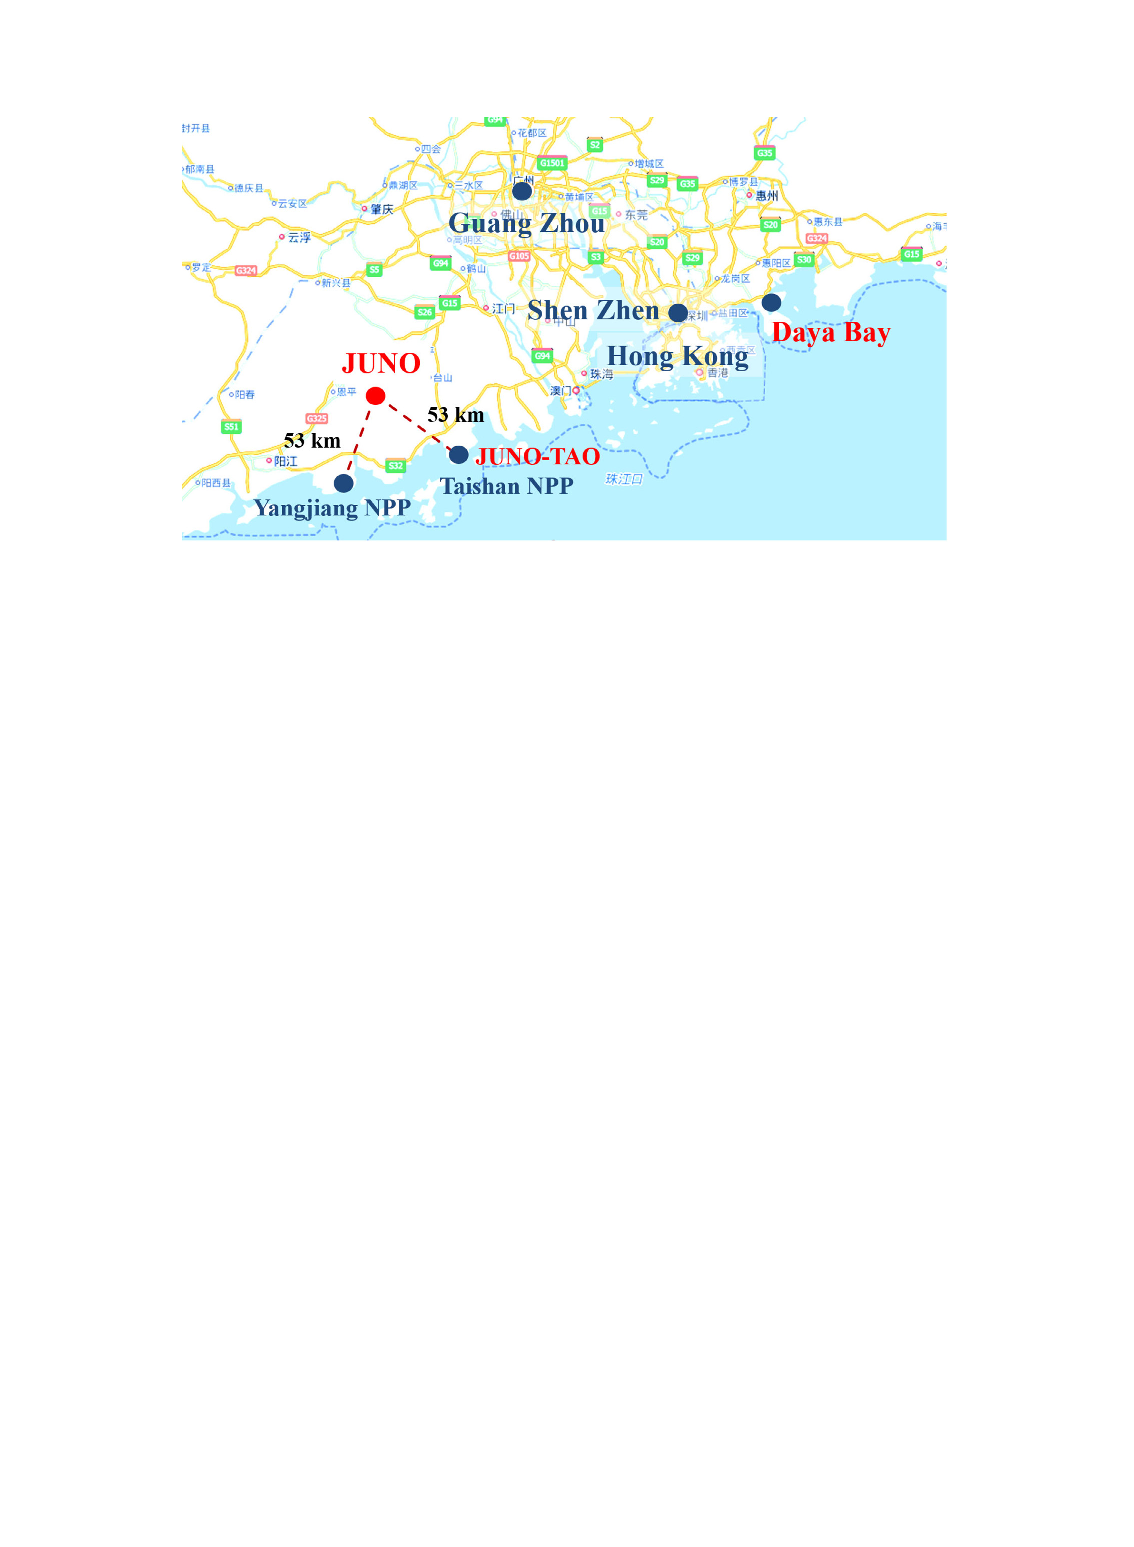
\includegraphics[width=0.7\textwidth]{junoDetector/location.pdf}
	\caption{The location of JUNO~\cite{muon207}: Jinji, Kaiping city, Jiangmen city, Guangdong province, China. Its geographical location is $112^{\circ}31^{\prime}05^{\prime\prime}~\mathrm{E}$ and $22^{\circ}07^{\prime}05^{\prime\prime}~\mathrm{N}$.}
	\label{fig:juno_site}
\end{figure}

\begin{table}[htbp]
	\centering % 表格居中
	\caption{The power of the reactor core and the baseline distance, the data comes from~\cite{juno_yellow_book}}
	\label{tab:juno_core}
	\begin{tabular}{cccccccc}
		\toprule % 顶线
		\textbf{Cores}     & YJ-C1 & YJ-C2 & YJ-C3 & YJ-C4 & YJ-C5 & YJ-C6 \\
		\midrule
		Power~(\si{GW})    & 2.9   & 2.9   & 2.9   & 2.9   & 2.9   & 2.9   \\
		Baseline~(\si{km}) & 52.75 & 52.84 & 52.42 & 52.51 & 52.12 & 52.21 \\
		\addlinespace
		\textbf{Cores}     & TS-C1 & TS-C2 & TS-C3 & TS-C4 & DYB   & HZ    \\
		\midrule
		Power~(\si{GW})    & 4.6   & 4.6   & 4.6   & 4.6   & 17.4  & 17.4  \\
		Baseline~(\si{km}) & 52.76 & 52.63 & 52.32 & 52.20 & 215   & 265   \\
		\bottomrule
	\end{tabular}
\end{table}

% \begin{figure}[htbp]
% 	\centering
% 	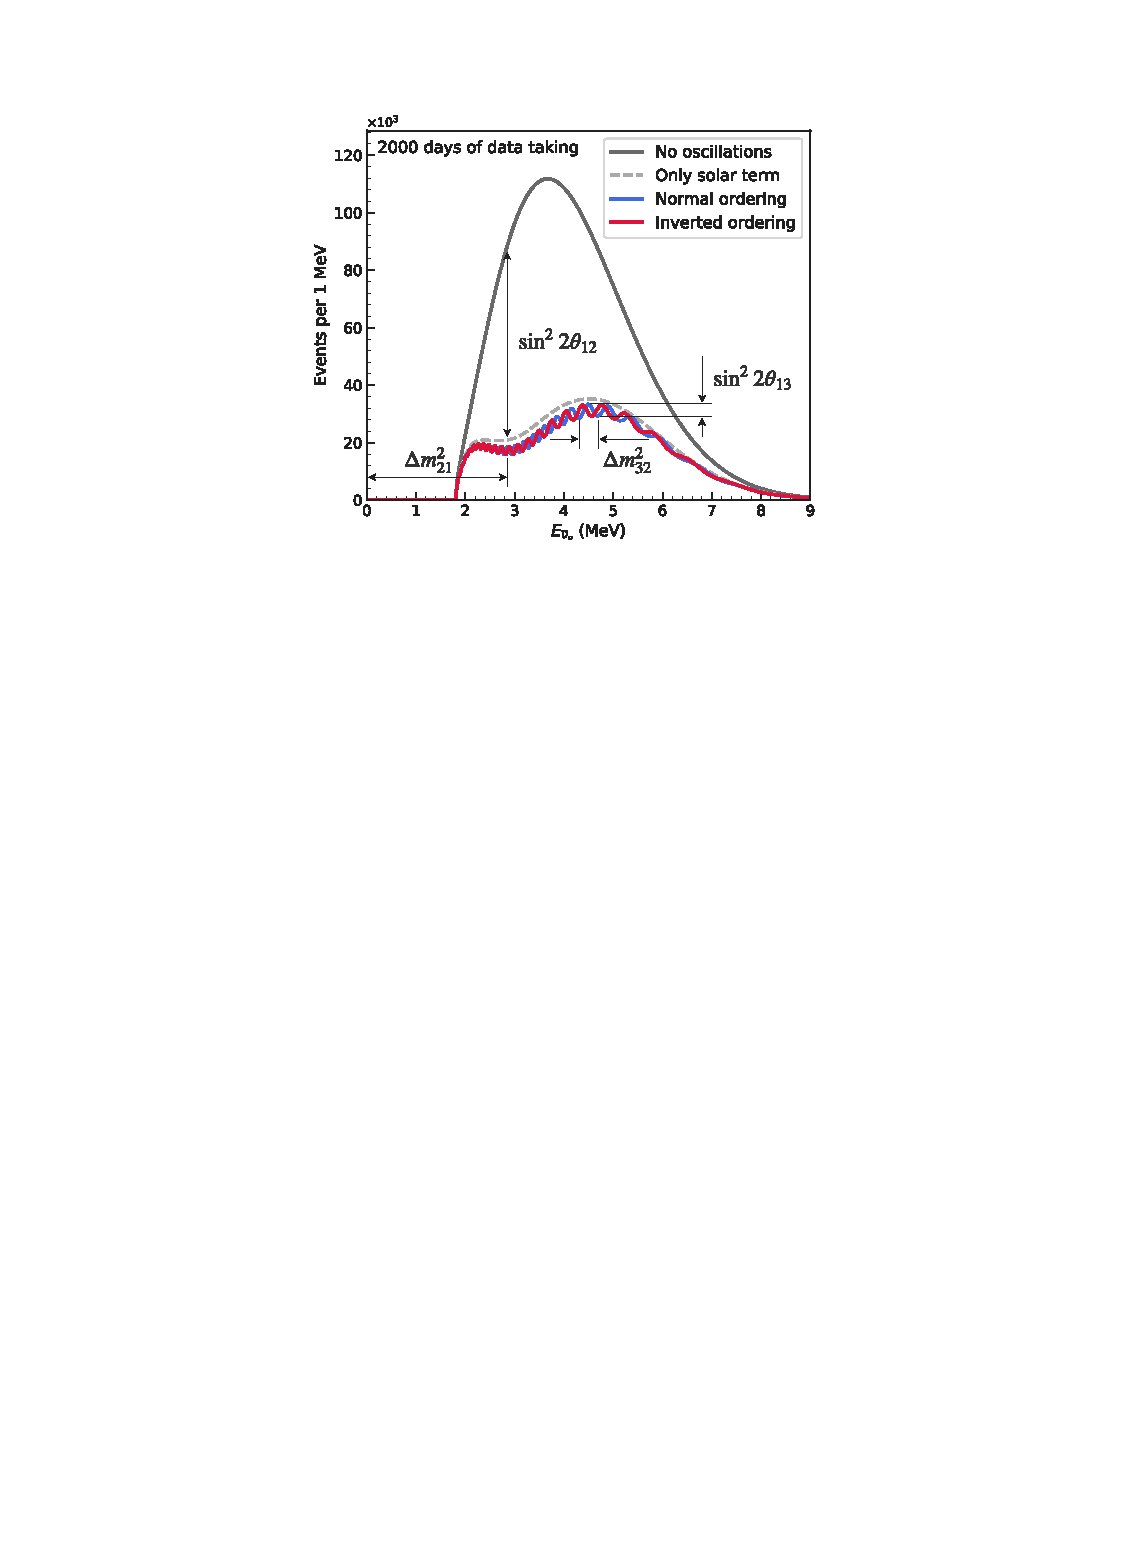
\includegraphics[width=0.5\textwidth]{junoDetector/nmo_2000day.pdf}
% 	\caption{The sensitivity of NMO measurement at JUNO after 2000 days of data taking based on simulation. Four oscillation parameters are depeended on~\cite{muon207}.}
% 	\label{fig:juno_nmo_2000}
% \end{figure}

\section{The design of JUNO Central Detector}
\label{sec:juno_cd_design}
The JUNO detector is composed of CD, a water Cherenkov detector based on the water pool~(WCD), and a Top Tracker~(TT), as illustrated in Fig.~\ref{fig:juno_cd_structure}.
\begin{figure}[htbp]
	\centering
	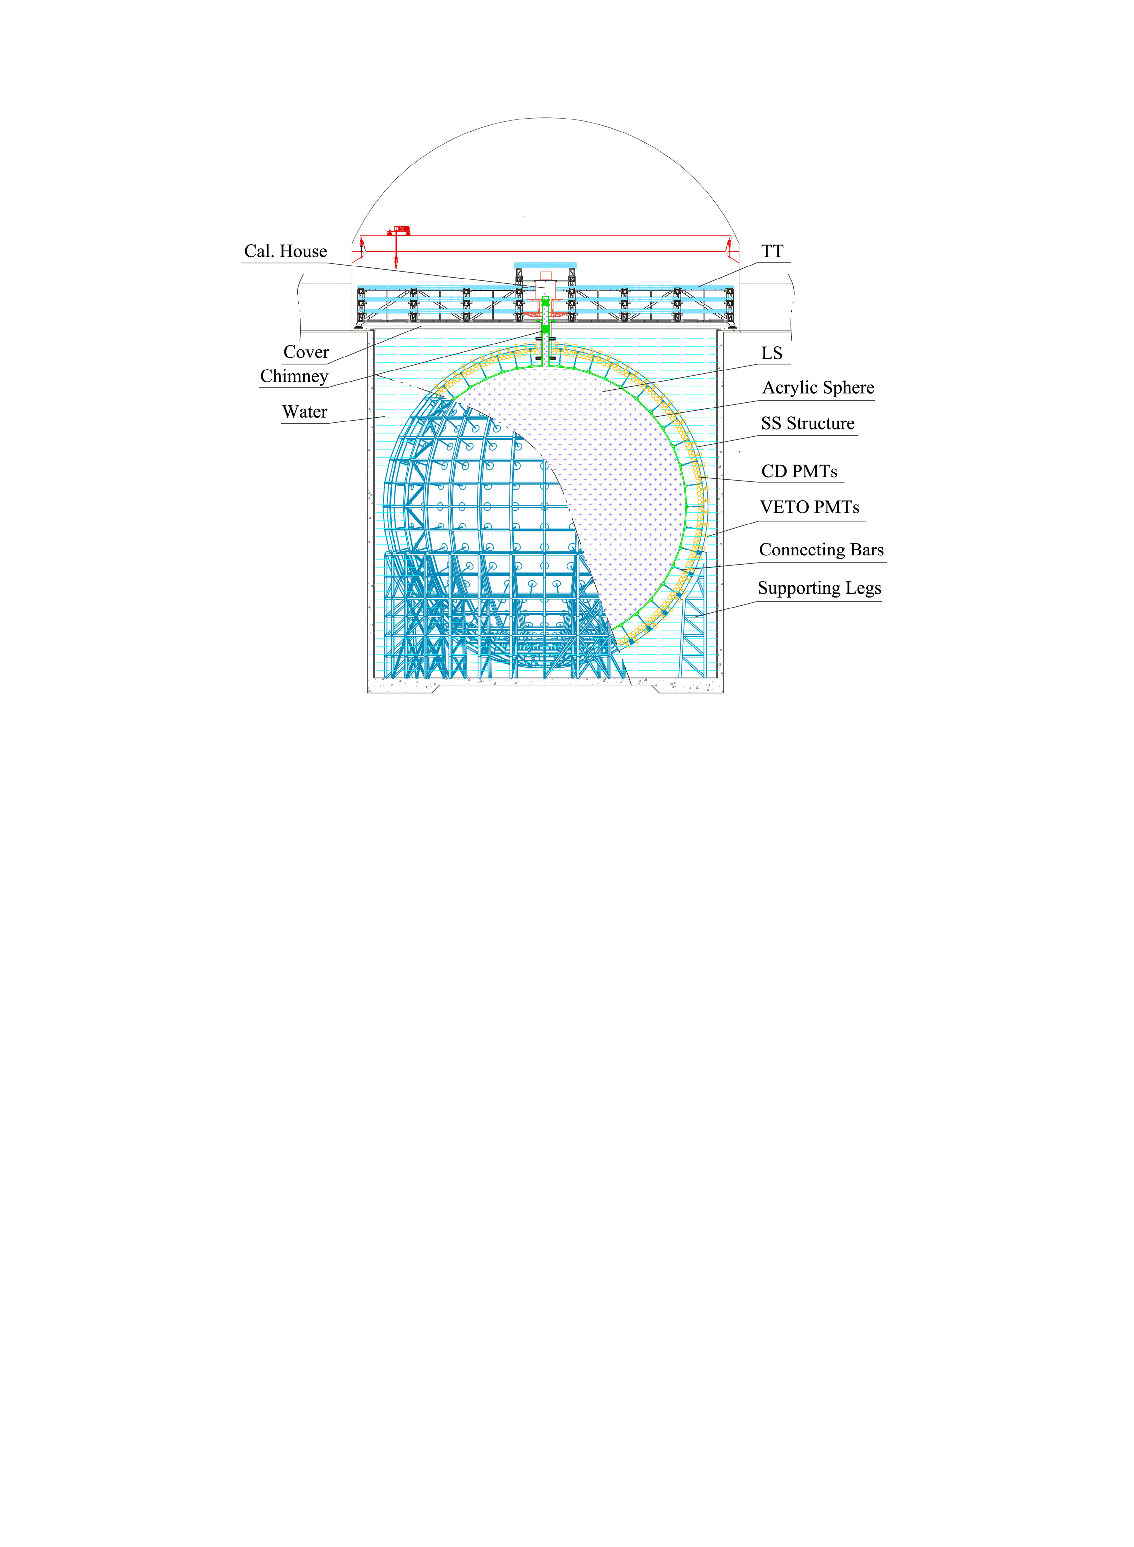
\includegraphics[width=0.6\textwidth]{junoDetector/structure.pdf}
	\caption{The structure of JUNO detector. The figure comes from~\cite{muon207}}
	\label{fig:juno_cd_structure}
\end{figure}
\subsection{The structure of Central Detector}
The Central Detector consists of an acrylic spherical shell with a diameter of \SI{35.4}{m} and a thickness of \SI{12}{cm}, which is filled with \SI{20}{kton} of liquid scintillator~\cite{JUNO_CD_tech}. It is engineered to attain an energy resolution of $\frac{\SI{3}{\%}}{\sqrt{E}}$ to facilitate the measurement of NMO. To detect the photons emitted due to the energy deposited by particles, 17,612 20-inch and 25,600 3-inch photomultiplier tubes~(PMTs), more detailed information in Tab.~\ref{tab:juno_pmt}, are mounted on a spherical structure with a radius of \SI{19.5}{m}. This setup achieves a photocathode coverage rate of over \SI{75}{\%}. Ultra-pure water is filled between the PMT and the acrylic to shield the radioactive background from the surface of the PMT. The entire CD detector is immersed in a cylindrical water pool to shield the radioactive background from the surrounding rocks, etc. At the same time, the water pool, as a Cherenkov detector, is equipped with 1,600 20-inch PMTs, enabling the detection of \SI{99.8}{\%} of cosmic muons. To avoid the interference of the geomagnetic field, a set of 32 circular coils surrounding the detector is designed to keep the residual magnetic field in the PMT area of CD less than \SI{0.05}{G} and that in WCD below \SI{0.1}{G}~\cite{muon207}.

\begin{table}[htbp]
	\centering % 表格居中
	\caption{The summary of PMTs used in JUNO CD, the data comes from~\cite{muon207,PMT-3inch,JUNO:2022hlz}}
	\label{tab:juno_pmt}
	\begin{tabular}{cccccccc}
		\toprule % 顶线
		    & Size~(\si{inch}) & Type       & Number & Manufacturer                               \\
		\midrule % 中线
		CD  & 20               & MCP-PMT    & 12612  & Northern Night Vision Technology Co.       \\
		    &                  & Dynode-PMT & 5000   & Hamamatsu Photonics K. K.                  \\
		    & 3                & SPMT       & 25600  & Hainan Zhanchuang Photonics Technology Co. \\
		WCD & 20               & MCP-PMT    & 2400   & Northern Night Vision Technology Co.       \\
		\bottomrule % 底线
	\end{tabular}
\end{table}

\subsection{The Top Tracker}
It is mainly used to reconstruct and track the trajectories of atmospheric muons. This detector is modified from the target tracker modules of the decommissioned OPERA experiment. It covers approximately \SI{60}{\%} of the area at the top of CD and contains 63 double-layer scintillator walls~(a total of 496 modules), as shown in Fig.~\ref{fig:TT_0}. Each module is composed of plastic scintillator strips arranged orthogonally, and the signals are read out through wavelength-shifting fibers connected to multi-anode PMTs~(MA-PMTs), as illustrated in Fig.~\ref{fig:juno_TT}. To adapt to the highly radioactive environment of the underground laboratory, its electronics system has been comprehensively upgraded to achieve precise triggering at high counting rates. TT can significantly reduce the interference of cosmic muon spallation background on the measurement of NMO through the reconstruction of muon trajectories with centimeter-level accuracy. It is particularly crucial for identifying the \ce{^9Li}/\ce{^8He} background induced by muons~\cite{top_tracker,muon207}.

\begin{figure}[htbp]
	\centering
	\begin{subfigure}{0.75\textwidth}
		\centering
		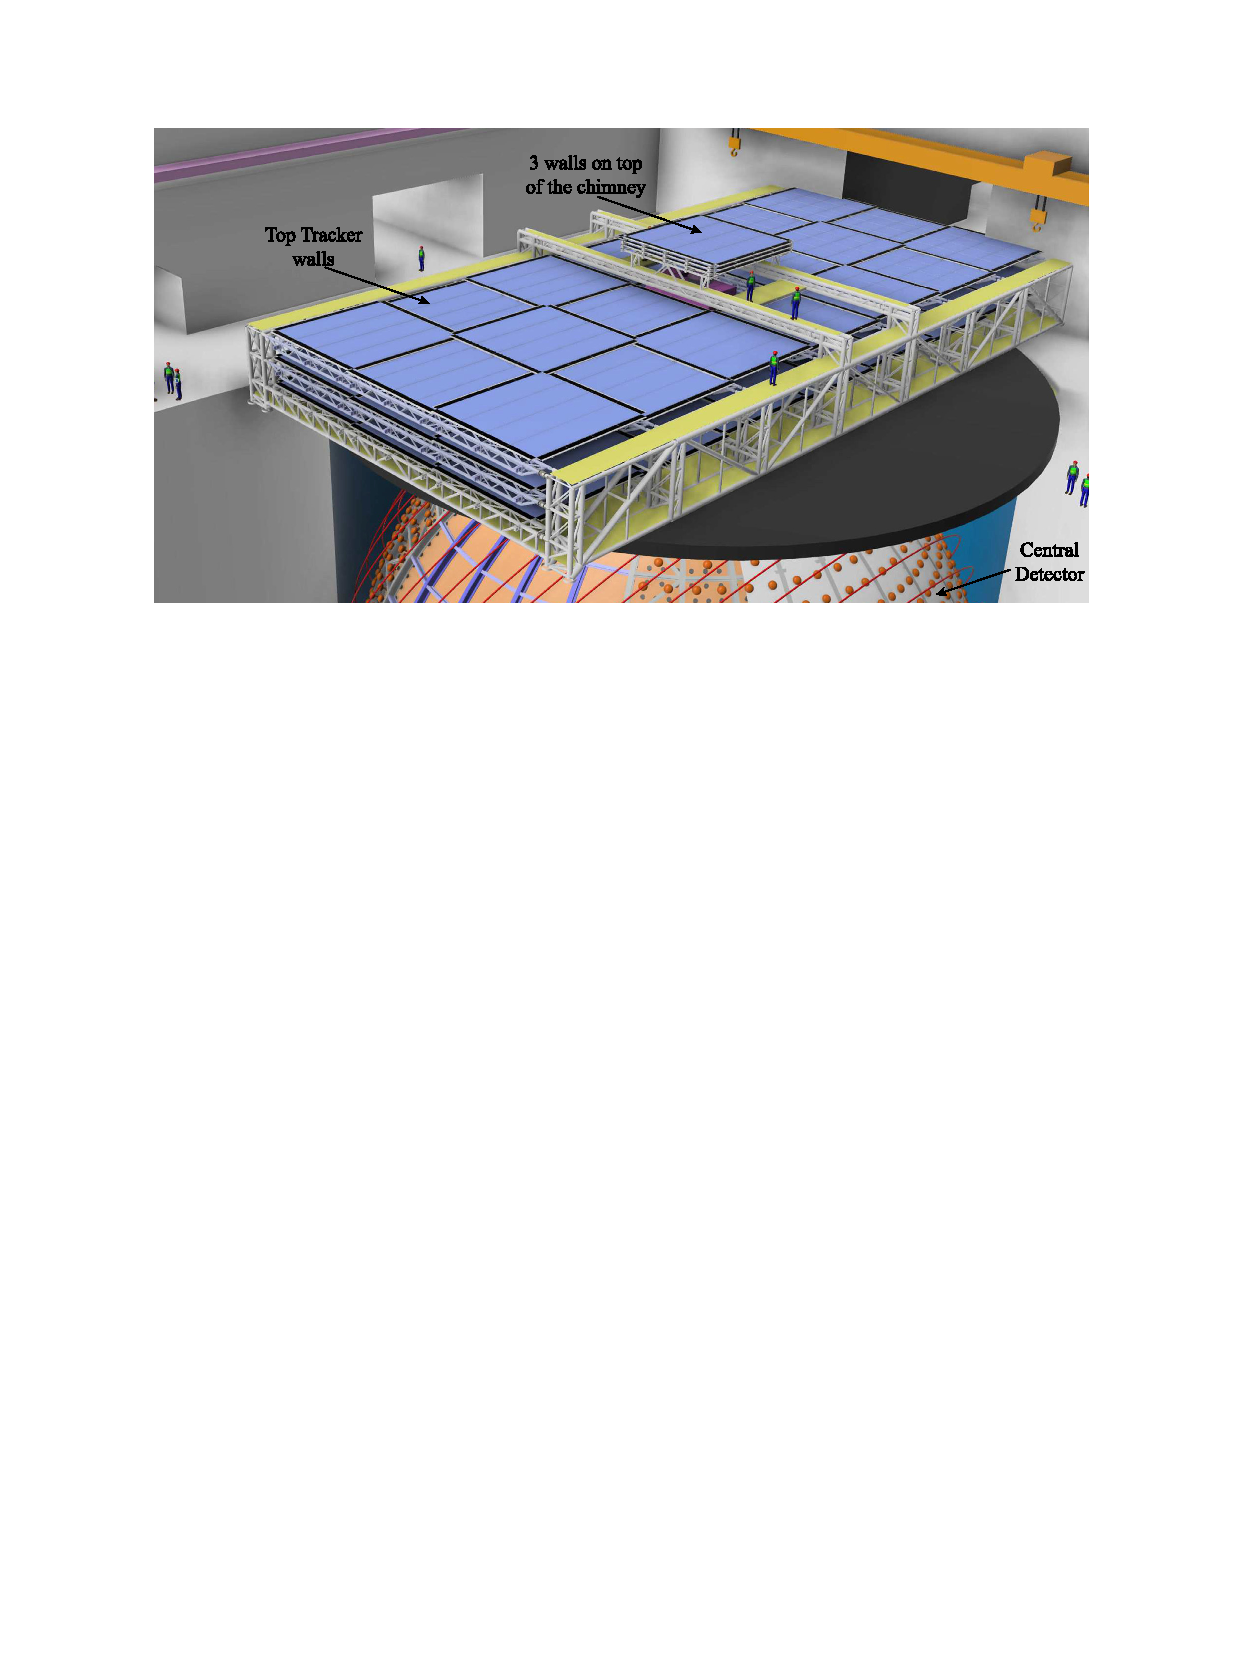
\includegraphics[width=\textwidth]{junoDetector/TT_0.pdf}
		\caption{}
		\label{fig:TT_0}
	\end{subfigure}%
	\hfill
	\begin{subfigure}{0.5\textwidth}
		\centering
		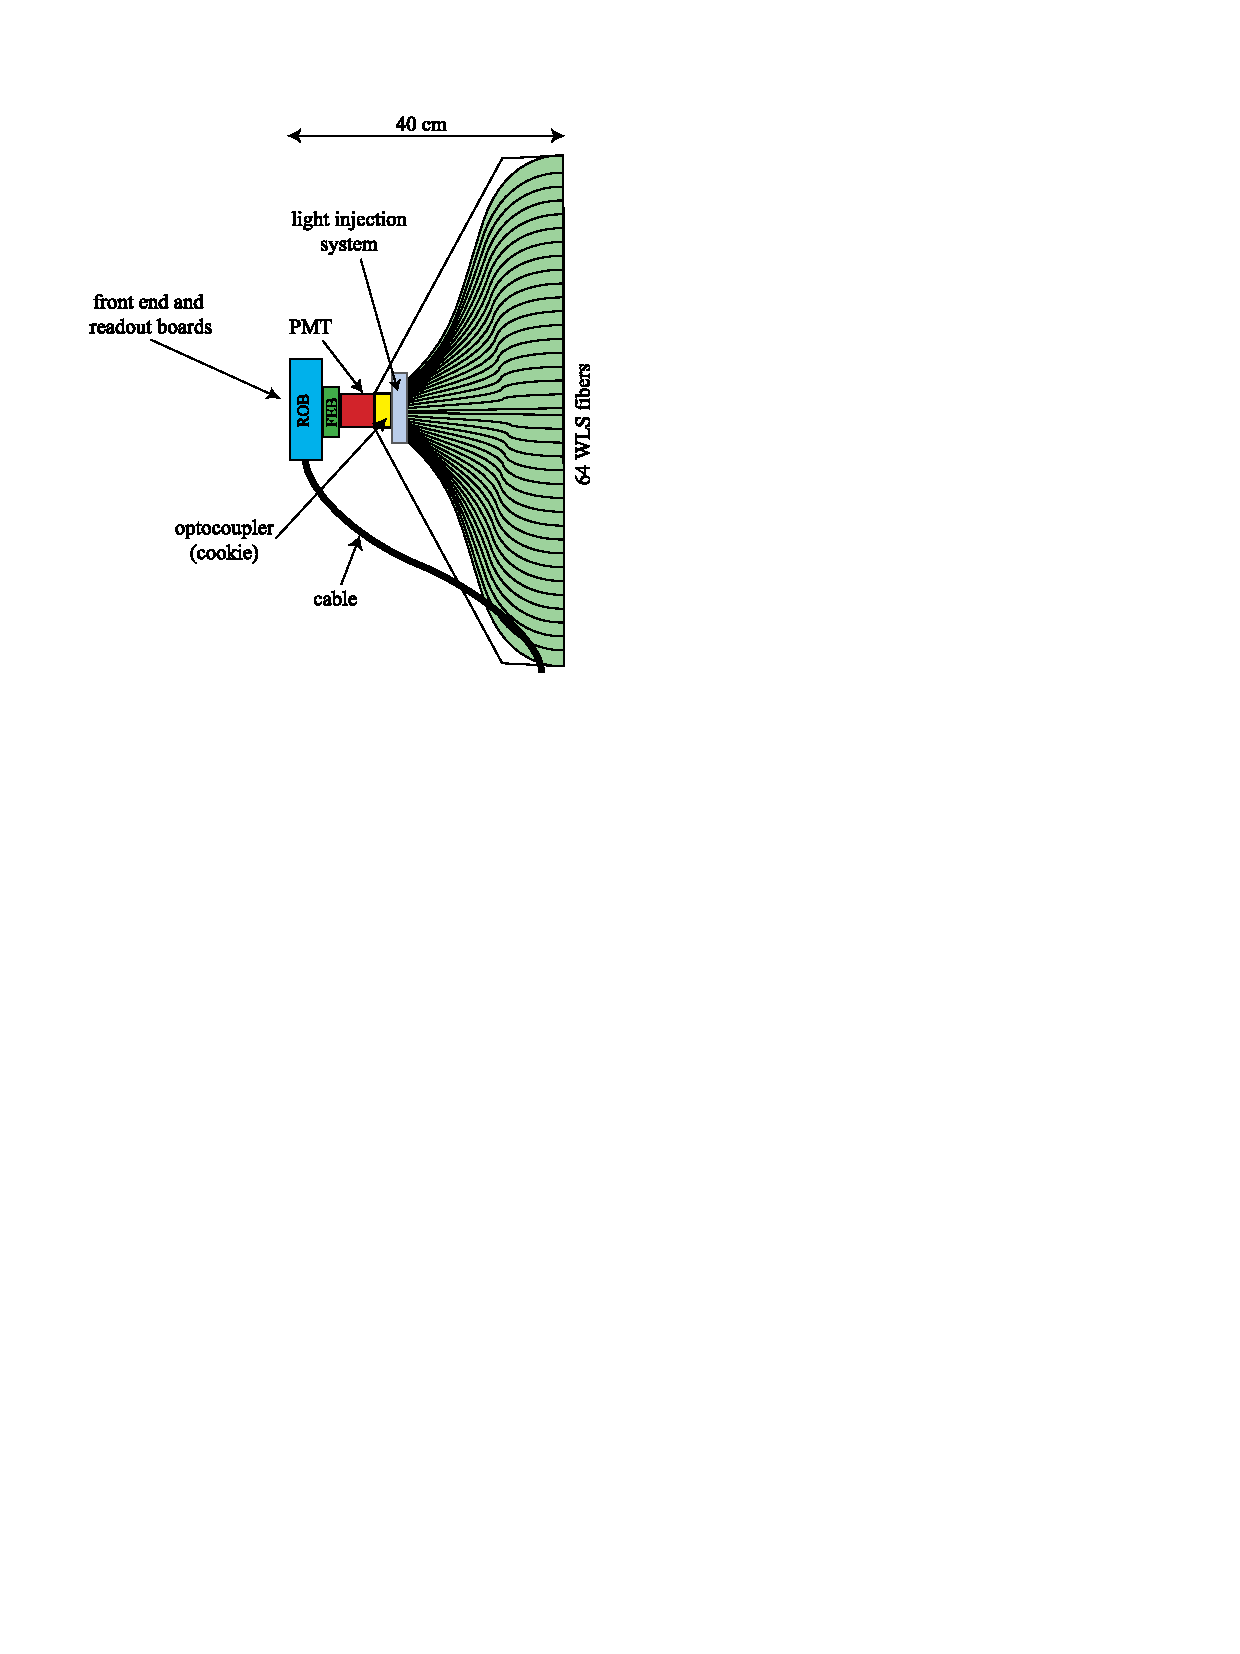
\includegraphics[height=6cm]{junoDetector/TT_1.pdf}
		\caption{}
		\label{fig:TT_1}
	\end{subfigure}%
	\hfill
	\begin{subfigure}{0.5\textwidth}
		\centering
		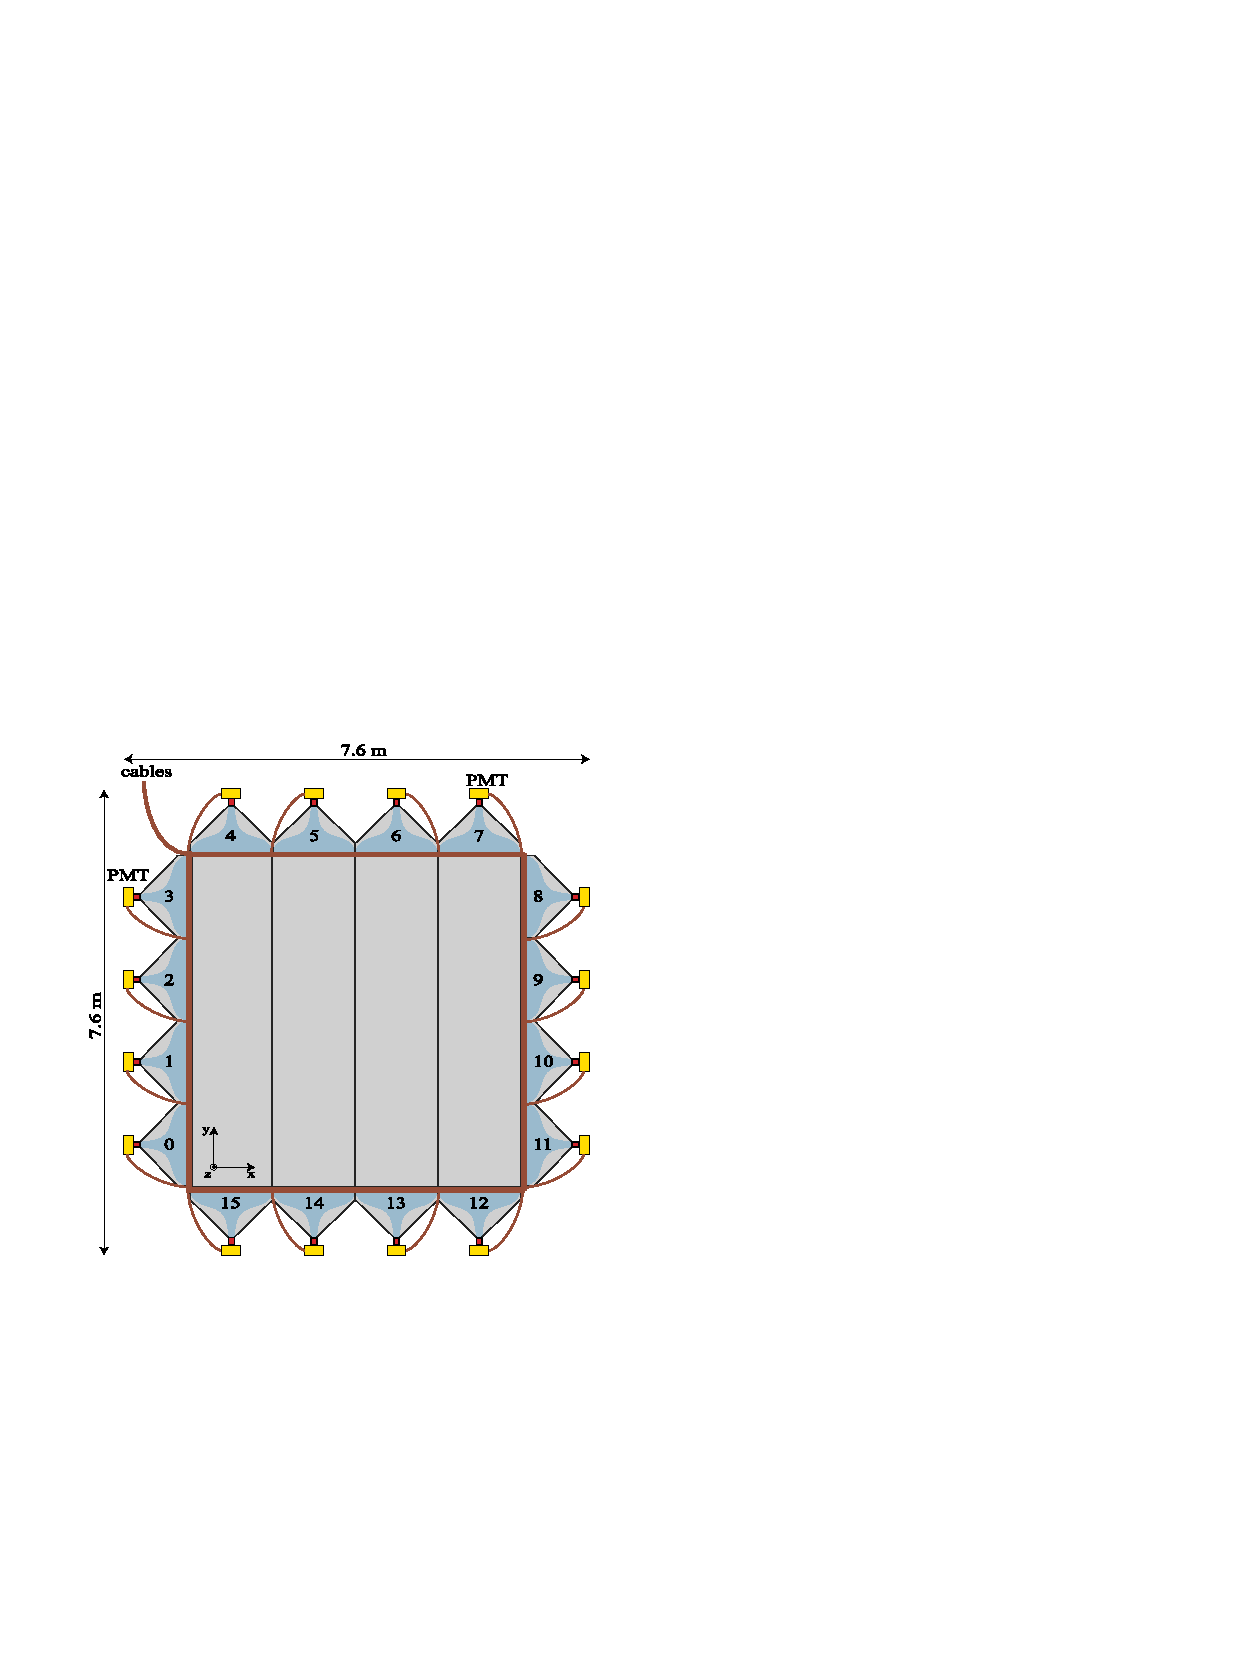
\includegraphics[height=6cm]{junoDetector/TT_2.pdf}
		\caption{}
		\label{fig:TT_2}
	\end{subfigure}
	\caption{\subref{fig:TT_0} presents the side view of TT from the CD side. \subref{fig:TT_1} is a schematic illustration of a TT module. This module is composed of 64 strips that are read out by WLS fibers and \subref{fig:TT_2} depicts a plastic scintillator strip wall. These figures are sourced from~\cite{top_tracker}.}
	\label{fig:juno_TT}
\end{figure}

\section{The trigger system of JUNO CD}
\label{sec:juno_trigger}
\subsection{The Multi-Messenger Trigger}
To efficiently and accurately select the physics events of interest from the large volume of detector data, the JUNO experiment has implemented several trigger systems. As a crucial component of the data acquisition chain, the trigger system directly impacts event recording efficiency, data quality, and the effectiveness of subsequent physics analyses. The Multi-Messenger~(MM) trigger~\cite{MMtrigger} is designed to enable the detection of low-energy events that are relevant to both neutrino and astrophysical physics.
In contrast to the multiplicity-based Global Trigger, which mainly depends on the number of detected photons within a single time window to initiate an event readout, MM Trigger is based on a number of likelihood and machine-learning, using the PMT timing and position information. It enables the detection of low-energy events that are relevant to both neutrino and astrophysical physics, and optimizes the discrimination between physics events and dark noise induced events to reduce the data volume.
\subsection{The Multiplicity Software Trigger}

\section{The calibration system in JUNO}
\label{sec:juno_calibration}
\subsection{The laser calibration}
\subsection{The position and uniformity calibration}
\subsection{The energy calibration}

\section{The Simulation Software of JUNO CD}
\label{sec:juno_simulation}
\section{The subdetector of JUNO}
\label{sec:juno_subdetector}
In the measurement of NMO, two extremely crucial factors are the input reactor neutrino energy spectrum and the purity of LS. JUNO has designed a sub-detector TAO at Taishan to provide an accurate input energy spectrum. During the liquid scintillator filling period, in order to detect the background content of LS, the OSIRIS detector has been designed and operated beside the JUNO CD.

\subsection{The Taishan Antineutrino Observatory}
The Taishan Antineutrino Observatory~(TAO) serves as a satellite detector of JUNO. It is positioned \SI{30}{m} away from the reactor core of the Taishan Nuclear Power Plant. The core of TAO consists of a spherical acrylic vessel with a diameter of \SI{1.8}{m}, which is filled with \SI{2.8}{m^3} of gadolinium-doped liquid scintillator~(Gd-LS)~\cite{TAO_wangzhimin}, as shown in Fig.~\ref{fig:tau_structure}. This detector innovatively employs a \SI{10}{m^2} silicon photomultiplier~(SiPM) array to fully cover the spherical vessel. When combined with the \SI{-50}{\degreeCelsius} cryogenic operation technology, the dark noise is significantly reduced, achieving an ultra-high collection efficiency of \SI{4500}{PE/MeV}. After an effective volume with a radius of \SI{1.3}{m}, a revolutionary energy resolution of $2\%/\sqrt{E}$ is realized~\cite{TAO_wangzhimin}. Combined with high statistics, TAO will measure the reactor neutrino energy spectrum more accurately and with lower uncertainty than CD, as illustrated in Fig.~\ref{fig:tau_uncertainty}. It will provide an important reference energy spectrum for JUNO to determine NMO~\cite{Tao_design}. At the same time, TAO can also verify nuclear databases and explore applications in reactor monitoring.
\begin{figure}[htbp]
	\centering
	\begin{subfigure}{0.5\textwidth}
		\centering
		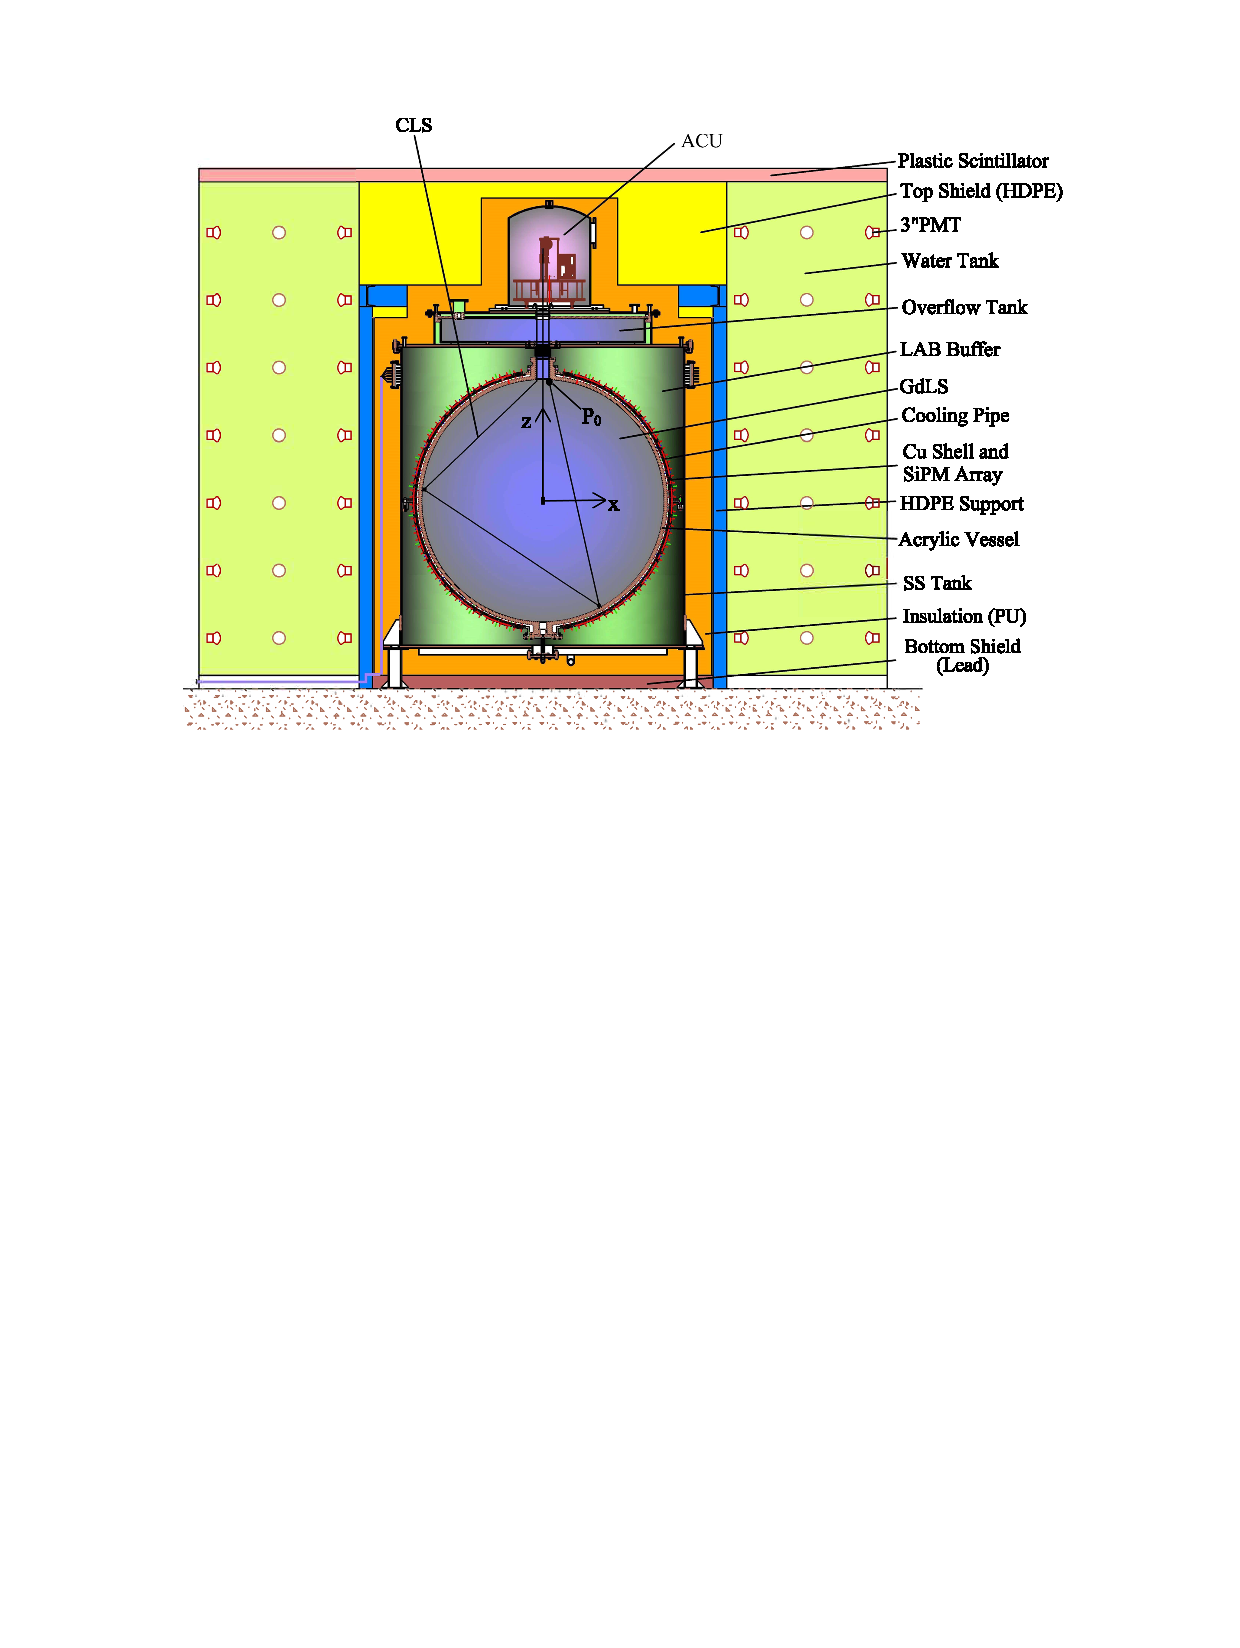
\includegraphics[height=5cm]{junoDetector/TAO_structure.pdf}
		\caption{}
		\label{fig:tau_structure}
	\end{subfigure}%
	\hfill
	\begin{subfigure}{0.5\textwidth}
		\centering
		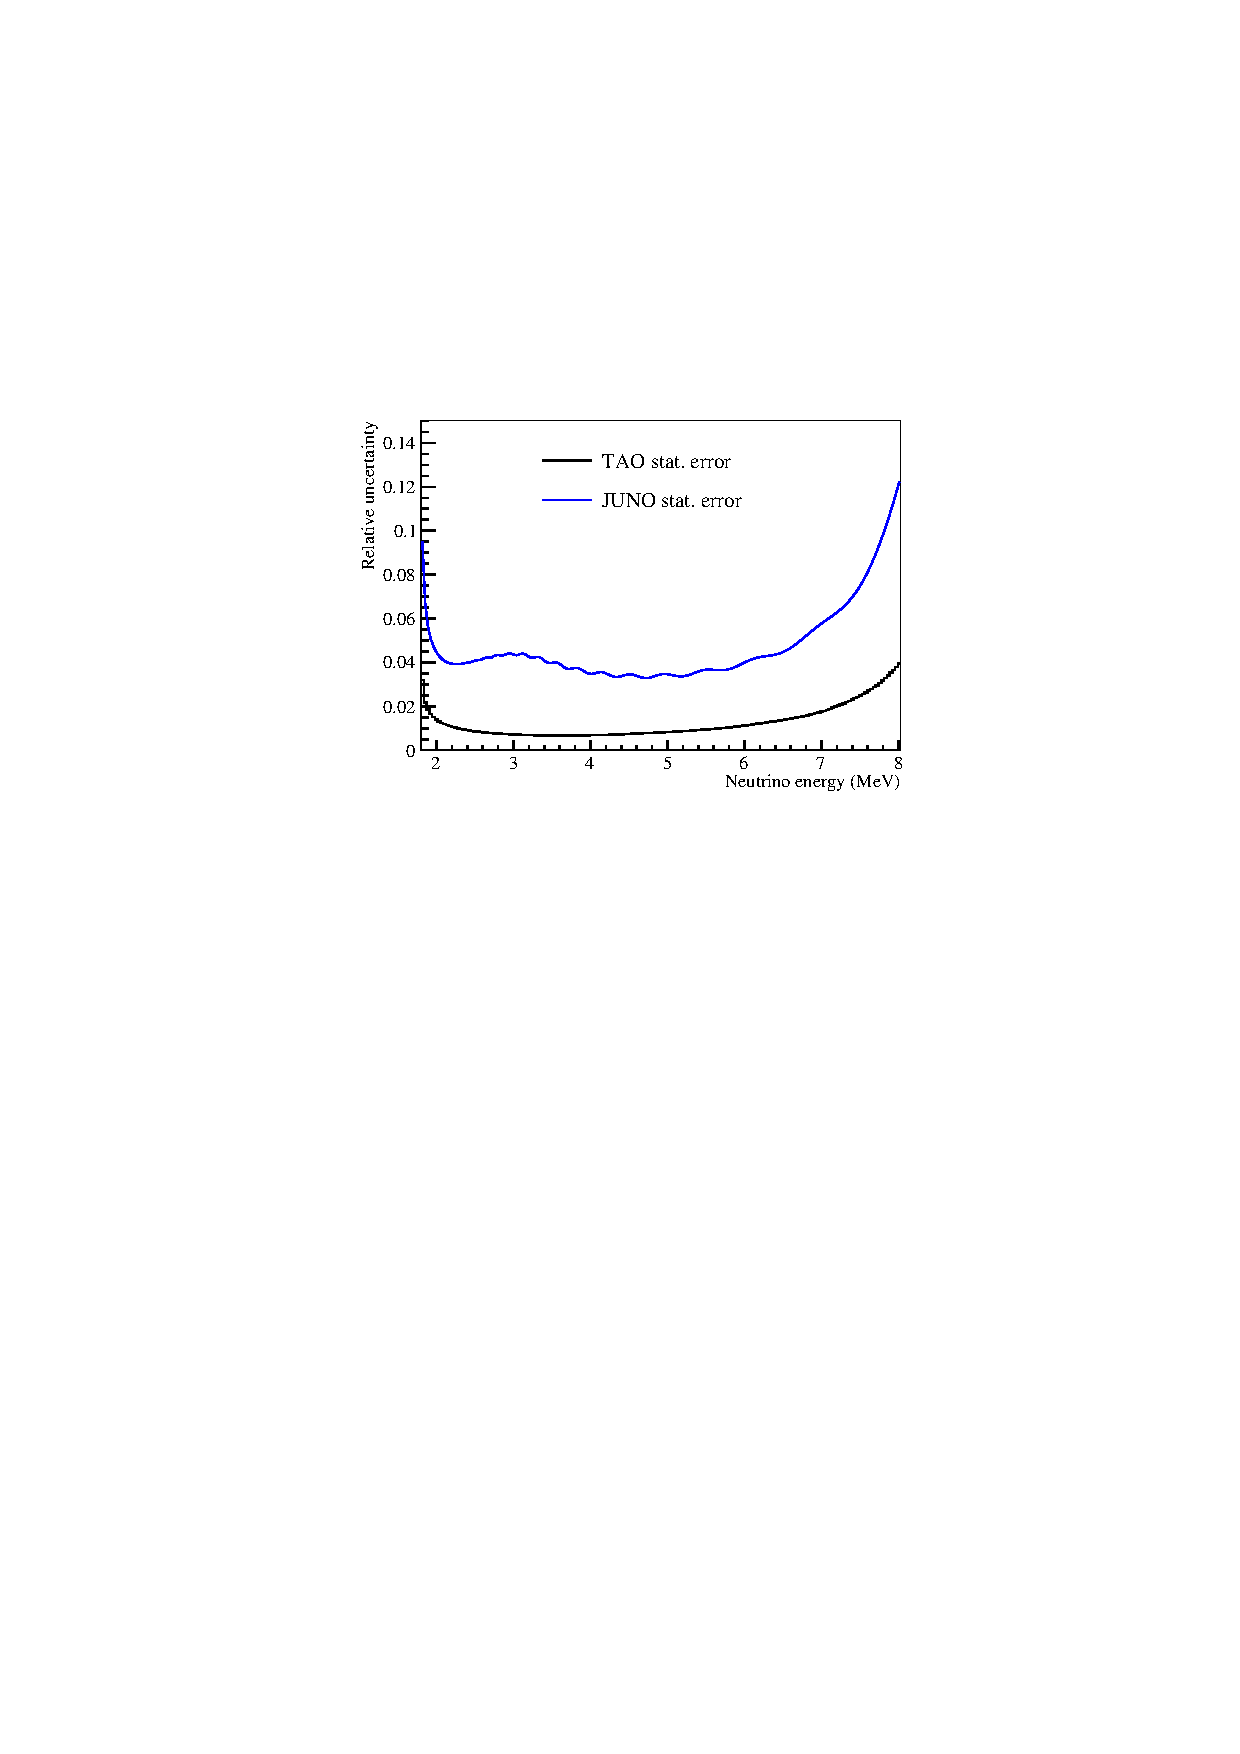
\includegraphics[height=4.5cm]{junoDetector/TAO_uncertainty.pdf}
		\caption{}
		\label{fig:tau_uncertainty}
	\end{subfigure}
	\caption{\subref{fig:tau_structure} presents the structure of TAO, this figure comes from~\cite{TAO_calib}. \subref{fig:tau_uncertainty} is showing the uncertainty of energy spectrum at JUNO CD and TAO, this figure comes from~\cite{Tao_design}.}
	\label{fig:juno_tao}
\end{figure}
\subsection{The Online Scintillator Internal Radioactivity Investigation System}
The Online Scintillator Internal Radioactivity Investigation System~(OSIRIS)
\section{The JUNO detector during water phase}
\label{sec:juno_water}
\chapter{The PMT calibration in water phase}\label{sec:Introduction}

\section{The single electron response of MCP-PMTs}
The photomultiplier tubes~(PMT) see extensive deployments in particle physics, particularly neutrino experiments.
A PMT comprises a photocathode, an electron multiplier, an anode, and other necessary structural components~\cite{1955Scintillation}.
Photons from a light source incident on the photocathode follow a Poisson process.
Some of them are converted to photoelectrons~(PE) via the photoelectric effect
and such PEs enter the multiplier~\cite{2016Optimization}.
Those two processes are Bernoulli selections, with the probabilities known as the \emph{quantum efficiency}~(QE) and the \emph{collection efficiency}~(CE).
The PE count~($n_{\mathrm{PE}}$) in a specific time interval follows a Poisson distribution~\cite{1994Absolute}.

The electron amplification is driven by the secondary electron emission~(SEE).
When an incident particle, such as electron and ion, collides with or goes through a solid surface, one or more secondary electrons are emitted~\cite{2016Secondary}.
The average number of secondaries produced per incident particle is the secondary-emission yield~(SEY, $\delta$).
The energy distribution of the secondaries~(\(\mathrm{d}\delta/\mathrm{d}E\)) is related to the energy of the incoming particle,
the incident angle, the target material, etc.~\cite{2002Probabilistic}.
Bruining and Boer~\cite{1938Secondary}, Ushio~et~al.~\cite{1988Secondary} and Jokela~et~al.~\cite{2012Secondary}
conducted target-shooting experiments using electron guns,
and measured the SEY in the current mode.
Olano and Montero~\cite{OLANO2020103456} measured the energy distribution \(\mathrm{d}\delta/\mathrm{d}E\) of Kapton, Teflon, and Ultem by charging analysis,
and found the energy of secondaries to be much smaller than that of the primary electrons.
Such results are then extrapolated to PMTs~\cite{2012An,2021Effects}.
The low light intensity at which a PMT operates makes the incident electrons discrete.
Therefore, one should be careful when extending the SEY from the current mode to a single electron case, the pulse mode.

While being amplified by the multiplier,
a single PE induces numerous electrons,
which are captured by the anode within a few hundred picoseconds.
The initial energy of the PEs produced at the photocathode is \SI{\sim 1}{eV}~\cite{Nathan1970TheED}.
The potential difference between the photocathode and the multiplier dominates the incident energy of the PEs arriving at the multiplier.
Therefore, the amplifier provides nearly identical gain for the PEs.
Because the total charge of the electrons captured by the anode is typically described by a Gaussian distribution in light of the central limit theorem of probability,
the probability density function~(PDF) of the single electron response~(SER) charge distribution is $f_{\mathcal{N}}(Q; Q_1,\sigma_1^2)$,
where $Q_1$ is the mean charge, and $\sigma_1$ is its standard deviation.
The PE count $n_{\mathrm{PE}}$ follows a Poisson distribution with the probability mass function $P_\pi(n_{\mathrm{PE}};\lambda)$,
where $\lambda$ is the expected PE count at a certain light intensity.
After amplification, the total charge distribution $f(Q)$ is a folding of the Poisson distribution and the SER charge distribution~\cite{1994Absolute}.
There are two types of background processes.
The first one follows a low-charged finite-width Gaussian~$\mathcal{N}(0,\sigma_0^2)$ without any PEs emitted from the photocathode.
The second process is discrete with a probability $w$.
Examples include thermoemission and noise generated by incident light.
This discrete process follows an exponential distribution~$\mathrm{Exp}(\alpha)$,
with $\alpha$ being the rate of exponential decay.
Considering the charge distribution of the two types of background processes being $f_{\mathrm{b}}(Q)$,
the overall charge distribution can be expressed in Eq.~(\ref{eq:sreal}):
\begin{equation}
	\begin{aligned}
		f(Q) =  & P_{\pi}(n_{\mathrm{PE}}=0;\lambda)f_{\mathrm{b}}(Q) + \sum_{n_{\mathrm{PE}}=1}^{\infty}P_{\pi}(n_{\mathrm{PE}};\lambda) f_{\mathcal{N}}(Q; n_{\mathrm{PE}}Q_1,n_{\mathrm{PE}}\sigma_1^2) \\
		\approx & \left\{\frac{(1-w)}{\sigma_0 \sqrt{2 \pi}} \exp \left(-\frac{Q^2}{2 \sigma_0^2}\right)
		+w \theta(Q)\times \alpha \exp \left(-\alpha Q\right)\right\} \mathrm{e}^{-\lambda}                                                                                                                \\
		        & +\sum_{n_{\mathrm{PE}}=1}^{\infty} \frac{\lambda^{n_{\mathrm{PE}}} \mathrm{e}^{-\lambda}}{n_{\mathrm{PE}} !}
		\times \frac{1}{\sigma_1 \sqrt{2 \pi n_{\mathrm{PE}}}}\times
		\exp \left(-\frac{\left(Q-n_{\mathrm{PE}} Q_1\right)^2}{2 n_{\mathrm{PE}} \sigma_1^2}\right)
	\end{aligned}
	\label{eq:sreal}
\end{equation}
where $\theta(Q)$ is the Heaviside function.
When $\lambda$ is less than 0.1,
the probability of observing two or more PEs is less than one-tenth of the probability of observing a single PE.
In this case, the charge distribution will only show the peak of the pedestal ($Q=0$) and the peak of the single PE ($Q=Q_1$) as indicated in the blue histogram in Fig~\ref{fig:spe_sreal}.
We can obtain an approximate SER charge spectrum after applying some cuts to remove the pedestal.
Our work aligns different PMTs' gain by dividing the SER charge spectrum with $Q_1$ as $Q/Q_1$.
\begin{figure}[!htbp]
	\centering
	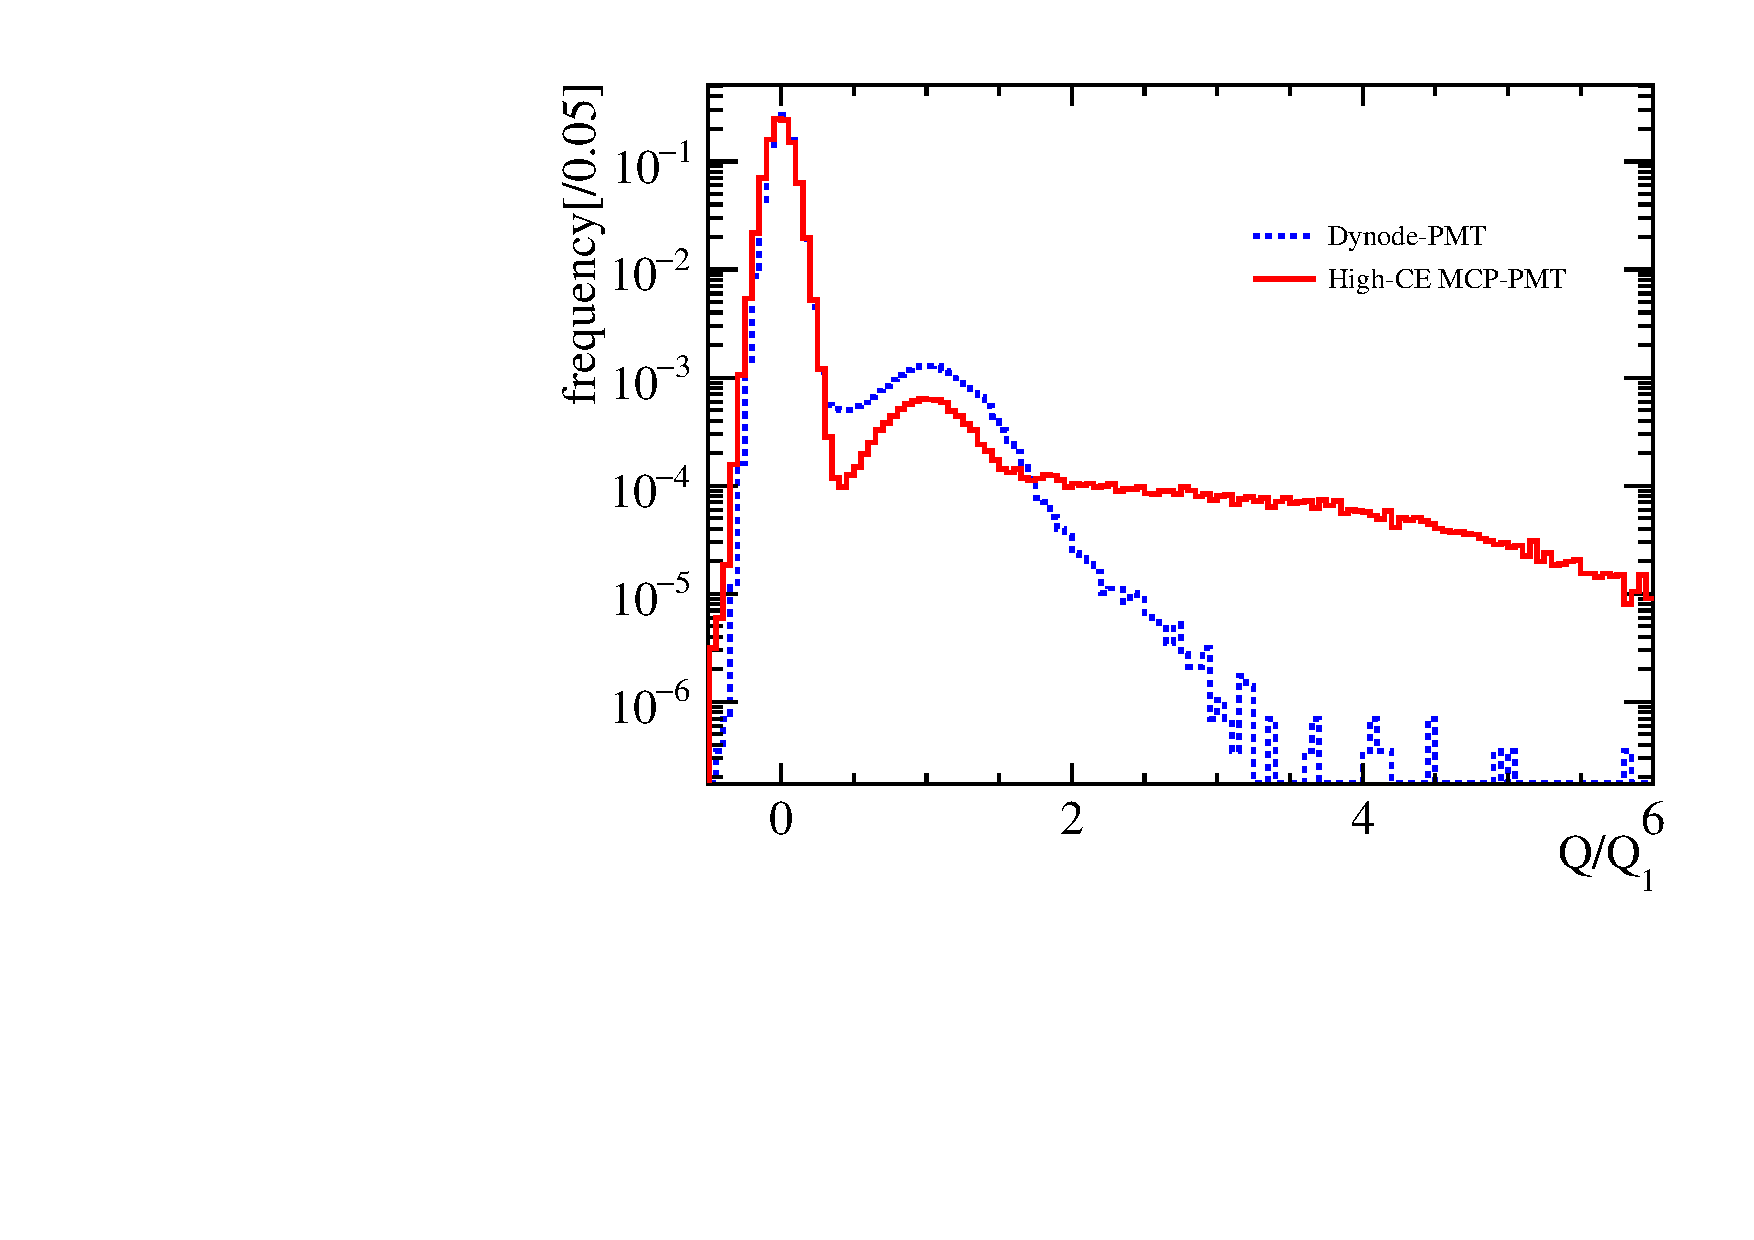
\includegraphics[width=0.5\textwidth]{PMTRelated/GTmodel/spe.pdf}
	\caption{The charge spectrum of the high-CE MCP-PMT GDB-6082~(red) and a dynode-PMT~(blue)~\cite{Zhang:2023ued}.
		The blue histogram consists of the pedestal $Q=0$ and the principal peak of $Q=Q_1$, while the red histogram includes jumbo charges.}
	\label{fig:spe_sreal}
\end{figure}
Instead of a large-sized dynode-chain commonly used in PMTs,
MCP-PMTs employ MCPs as electron multipliers.
MCP-PMTs are currently in use or planned for neutrino experiments
like the Jiangmen Underground Neutrino Observatory~(JUNO)~\cite{ZHU2020162002} and the Jinping Neutrino Experiment~\cite{Zhang:2023ued},
collider experiments like the Belle II TOP detector~\cite{MATSUOKA2014148} and the PANDA DIRC Cherenkov detector at FAIR~\cite{KRAUSS2023168659},
and cosmic ray observatories like the Large High Altitude Air Shower Observatory~\cite{Cao2019UpgradingPT}.
Initially, the fact that the feedback ions cause damage to the photocathode
led to a lifetime issue of MCP-PMTs~\cite{N2006Lifetime}.

The atomic layer deposition~(ALD) technique~\cite{2012An}
is applied to fabricate MCP-PMTs solving the lifetime issue~\cite{Lehmann:2022ret}.
Chen~et~al.~\cite{2016Optimization} indicated that depositing high SEY materials
such as \ce{Al2O3} via ALD on the input electrode of the first MCP
can enhance the probability of collecting the secondaries to improve CE
to nearly \SI{100}{\%} rather than being constrained by the MCP open-area ratio.
This enhancement is later extended to a composite \ce{Al2O3}-\ce{MgO} layer
by Cao~et~al.~\cite{cao_secondary_2021} and Zhang~et~al.~\cite{zzj2021Al}
to allow for increased gain, improved single electron resolution,
and a higher peak-to-valley ratio of the MCP-PMTs~\cite{2021Effects}.

In the performance tests to evaluate the 8-inch high-CE MCP-PMT by the Jinping Neutrino Experiment,
\emph{jumbo charges} are found in the SER charge spectra~\cite{Zhang:2023ued},
as shown in the red histogram in Fig~\ref{fig:spe_sreal}.
Similar charges have also been observed in the mass testing of the 20-inch MCP-PMTs at JUNO,
identified as the ``long tail'' in the SER charge distribution~\cite{JUNO:2022hlz}.
Orlov~et~al.~\cite{reviewer1} reported that the pulse height distribution of the high-CE MCP-PMTs had a non-Gaussian long-tail structure.
Zhang~et~al.~\cite{2021Gain} used the charge model in Eq.~\eqref{eq:sreal} for the jumbo charges and recommended an extra gain calibration.
Yang~et~al.~\cite{2017MCP} conducted a voltage-division experiment to reveal that the MCP gain for the low-energy electrons is significantly smaller than
that for the high-energy ones.
Thus, the MCP gain for the secondaries differs from that for the PEs entering the channels directly.
The SER charge model in Eq.~\eqref{eq:sreal} is no longer sufficient to accurately calibrate this type of PMT.
Understanding the origin of the jumbo charges is necessary for an appropriate SER charge calibration.


To elucidate the nature of the jumbo charges, the Gamma distribution is introduced and a voltage-division experiment is developed to measure the relationship
between MCP gain and the energy of the incident electrons.
Considering the SEE model, we elucidate the nature of the jumbo charges
and calculate the total SEY of the \ce{Al2O3}-\ce{MgO} layer when the incident energy is \SI{650}{eV}.
Through convolution-based modeling, the physical mechanisms driving have been clarified, and a quantitative mathematical framework establishe, which is the first formulation for these kind of high-CE MCP-PMTs.

\subsection{Gamma-Distributed SER charges}\label{gammapossion}
Every multiplication of electrons at the dynodes or MCP channels follows approximately a Poisson distribution~\cite{branchandPoisson}.
A series of such multiplications forms cascaded Poissonians~\cite{1955Scintillation} and is
an example of the branching process~\cite{Bartlett1963TheTO} challenging to perform analytical computations.
Woodward~\cite{Woodward} argued that the SER charge spectrum exhibits an intermediate shape between a Poisson and a Gaussian.
Prescott~\cite{polya} proposed a cascaded Polya distribution to characterize the electron multiplication in PMT,
particularly when considering the non-uniformity of the dynode surface.
Kalousis~\cite{2012Calibration,2020A} approximated the Polya distribution as a Gamma one to calibrate PMT
and achieved better results than the Gaussian model in Eq.~\eqref{eq:sreal}.

Instead of the Gaussian containing a small nonphysical tail less than 0,
we choose a Gamma distribution $\varGamma(\alpha, \beta)$
defined by the scale factor $\alpha$ and the rate factor $\beta$, as shown in Eq.~\eqref{eq:gamma}:
\begin{equation}
	\label{eq:gamma}
	\begin{aligned}
		f_\Gamma(x ; \alpha, \beta) = \frac{x^{\alpha-1} e^{-\beta x} \beta^\alpha}{\Gamma(\alpha)} \quad \text { for } x>0 \quad \alpha, \beta>0 \\
	\end{aligned}
\end{equation}
where $\Gamma(\alpha)$ is the Gamma function.
A Gamma distribution is uniquely determined by its expectation value \(\alpha/\beta=Q_1\) and variance \(\alpha/\beta^2=\sigma_1^2\),
which can be converted into the Gaussian counterparts in~Eq.~\eqref{eq:sreal}.
The charge spectrum based on the Gamma distribution is,
\begin{equation}
	\begin{aligned}
		f(Q) & = & P_{\pi}(n_{\mathrm{PE}}=0;\lambda)f_{\mathrm{b}}(Q) + \sum_{n_{\mathrm{PE}}=1}^{\infty}P_\pi(n_{\mathrm{PE}};\lambda) f_\Gamma(Q;n_{\mathrm{PE}}\alpha, \beta). \\
	\end{aligned}
	\label{eq:Gamma}
\end{equation}

\subsection{Jumbo Charges through Extra Multiplication}\label{sec:see}

SEE has received considerable attention during the widespread application of electronic tubes.
Bruining summarized the SEE's methods, findings, and applications in his classic \textit{Physics and Applications of Secondary Electron Emission}~\cite{bruining_physics_1954}.
Baroody~\cite{baroody1950theory} put forward his SEE theory of metals assuming that an incident primary
electron interacts only with free electrons in the conduction band,
without considering the variation of secondary emission with the primary energies.
Dekker~et~al.~\cite{dekker1952theory} presented the SEE quantum theory of
the Coulomb interaction between the incident primaries and the lattice electrons.
Wolff~\cite{wolff1954theory} provided the cascade theory for the diffusion, the energy loss, and the multiplication of
the secondary electrons within a metal.
Assuming both incident and back-scattered electrons within the target are isotropic,
Kanaya~et~al.~\cite{Kanaya_1978} calculated the SEY from insulators with the ionization potential
by setting the valence electron and the back-scattered coefficient
besides the parameter of the free-electron density effect.
Vaughan~\cite{vaughan} formulated the SEY
as a function of impact energy and direction used in computer programs, known as the \emph{Vaughan model}.
Furman and Pivi~\cite{2002Probabilistic} developed a mathematically self-consistent Monte Carlo program
to elucidate the SEE phenomenon from solid surfaces usually called the \emph{Furman model}.
This model incorporates the statistical nature of the SEE process
by considering the probability distribution governing the number of the secondaries emitted per incident primary electron.
The energies of secondary electrons are approximated as independent and identically distributed random variables
determined by the material properties and the primary energies.

Early models primarily focused on theoretical explanations of SEE.
The Vaughan and Furman models emphasize the Monte Carlo computation instead.
Comparatively, the Furman model strives for physical consistency and better agreement with experiments.
Therefore, we choose it for more adjustable parameters and higher accuracy.

\subsubsection{Furman probabilistic model}\label{subsec:fuman}

In the Furman model~\cite{2002Probabilistic}, there are three kinds of secondary electrons.
The first is the back-scattered electron, emitted through elastic scattering on the surface of the target material.
The energy distribution $\mathrm{d}\delta_{\mathrm{bs}}/\mathrm{d}E$ is defined in Eq.~\eqref{eq:backscatter},
where $\delta_{\mathrm{bs}}$ is the yield of the back-scattered electron,
the Heaviside function $\theta(E)$ ensures the $E<E_0$.
$E_0$ is the incident energy of the primary electron,
$\theta_0$ is the incident angle,
and $\sigma_{\mathrm{bs}}$ is an adjustable standard deviation.
\begin{equation}
	\label{eq:backscatter}
	\begin{aligned}
		 & \frac{\mathrm{d}\delta_{\mathrm{bs}}}{\mathrm{d}E} =\theta(E) \theta\left(E_0-E\right) \delta_{\mathrm{bs}}\left(E_0, \theta_0\right)
		\frac{2 \exp \left(-\left(E-E_0\right)^2 / 2 \sigma_{\mathrm{bs}}^2\right)}{\sqrt{2 \pi} \sigma_{\mathrm{bs}}
		\operatorname{erf}\left(E_0 / \sqrt{2} \sigma_{\mathrm{bs}}\right)}                                                                      \\
	\end{aligned}
\end{equation}

After penetrating the target material, some electrons are inelastically scattered by the atoms and are reflected out to form the second category.
Lenard called the bending of the electron track ``diffusion'',
and the trajectory turning $90^\circ$ as \text {``Rückdiffusion''} in German literature~\cite{bruining_physics_1954}.
Furman and Pivi~\cite{2002Probabilistic} adopted this convention to name them as the \emph{rediffused electrons}.
The energy distribution of the rediffused electrons is defined as Eq.~\eqref{eq:rediffused},
where $\delta_{\mathrm{rd}}$ is the yield of rediffused electron,
and $q$ is an adjustable parameter.
\begin{equation}
	\label{eq:rediffused}
	\begin{aligned}
		 & \frac{\mathrm{d}\delta_{\mathrm{rd}}}{\mathrm{d}E} =\theta(E) \theta\left(E_0-E\right) \delta_{\mathrm{rd}}\left(E_0, \theta_0\right) \frac{(q+1) E^q}{E_0^{q+1}} \\
	\end{aligned}
\end{equation}

The final and most important kind is the true-secondary electrons.
Upon deeper penetration of electrons into the target material, intricate physical processes ensue,
generating one or more secondaries.
This is the process of multiplying electrons.
The spectrum is defined as Eq.~\eqref{eq:true}.
\begin{equation}
	\label{eq:true}
	\begin{aligned}
		\frac{\mathrm{d} \delta_{\mathrm{ts}}}{\mathrm{d} E}=  \sum_{n=1}^{\infty}
		\frac{n P_{n,\mathrm{ts}}\left(n; \delta_{\mathrm{ts}}(E_0,\theta_0)\right)
		\left(E / \epsilon_{n}\right)^{p_{n}-1} e^{-E / \epsilon_{n}}}
		{\epsilon_{n} \Gamma\left(p_{n}\right) \Upsilon\left(n p_{n}, E_0 / \epsilon_{n}\right)}
		\times \Upsilon\left[(n-1) p_{n},\left(E_0-E\right) / \epsilon_{n}\right]
	\end{aligned}
\end{equation}
where $\delta_{\mathrm{ts}}(E_0,\theta_0)$
is the yield of the true-secondary electrons when the incident energy is $E_0$ and the incident angle is $\theta_0$,
$\epsilon_{n}>0$ and $p_{n}>0$ are the phenomenological parameters.
$\gamma(z,x)$ is the incomplete gamma function,
and $\Upsilon(z,x)=\gamma(z,x)/\Gamma(z)$ is the normalized form satisfying $\Upsilon(0,x)=1$.
$n$, the number of the true-secondary electrons, follows a Poisson distribution~$\mathrm{\pi}(\delta_{\mathrm{ts}}(E_0,\theta_0))$.
$P_{n,\mathrm{ts}}$ is its probability mass function.

As illustrated in Fig.~\ref{fig:SES}, we set the parameters as
$\delta_{\mathrm{bs}}=0.05$, $\delta_{\mathrm{rd}}=0.5$, $\delta_{\mathrm{ts}}=5$~\cite{2021Effects},
$\theta_0=0^\circ$  and $E_0=$\SI{650}{eV}.
The total spectrum is
$\mathrm{d}\delta/\mathrm{d}E=\mathrm{d}\delta_{\mathrm{bs}}/\mathrm{d}E+\mathrm{d}\delta_{\mathrm{rd}}/\mathrm{d}E+\mathrm{d}\delta_{\mathrm{ts}}/\mathrm{d}E$.
The energies of the secondaries are usually less than \SI{100}{eV} when the incident energy~$E_0$ is \SI{650}{eV}.
\begin{figure}[!htbp]
	\centering
	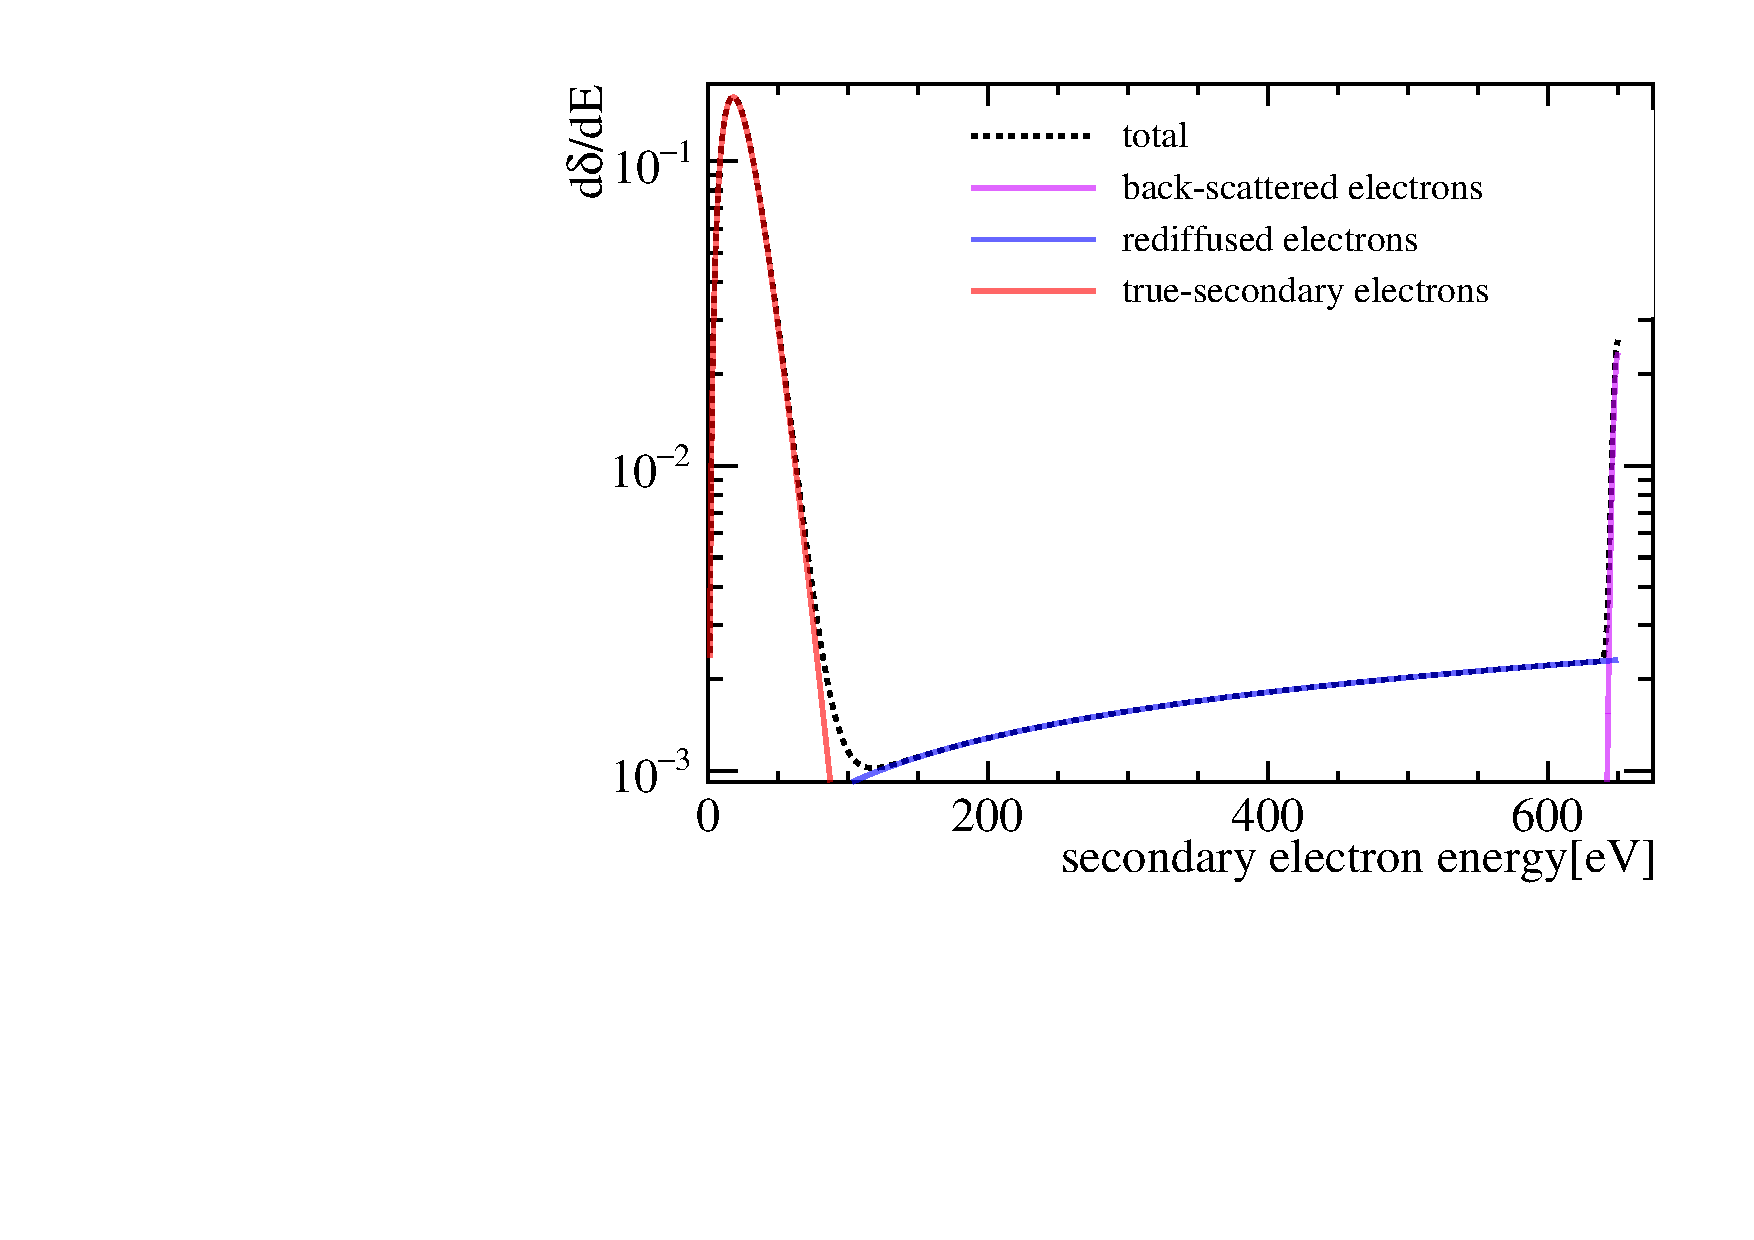
\includegraphics[width=0.5\textwidth]{PMTRelated/GTmodel/SES.pdf}
	\caption{The total energy spectrum of the secondary electrons when the incident energy is \SI{650}{eV}.
		The violet, blue, and red lines represent $\mathrm{d}\delta_{\mathrm{bs}}/\mathrm{d}E$, $\mathrm{d}\delta_{\mathrm{rd}}/\mathrm{d}E$, and
		$\mathrm{d}\delta_{\mathrm{ts}}/\mathrm{d}E$, repectively.
		The black dashed line is $\mathrm{d}\delta/\mathrm{d}E$.}
	\label{fig:SES}
\end{figure}

\subsubsection{An extra multiplication mode}
The MCP-PMT under study uses a Chevron stack of two MCPs as the electron multiplier.
As shown in Fig.~\ref{fig:circuit}, an \ce{Al2O3}-\ce{MgO}-\ce{Al2O3} layer~\cite{zzj2021Al} is deposited
on the channel surface of the lead glass body
and on the entrance electrode M1 of the first MCP through the ALD technology.
There are two alternative routes of amplification for every PE:
the \textit{channel mode}, where the PE directly enters a channel,
and the \textit{surface mode}, where the secondaries from $\mathrm{M}1$ enter the MCP channels under the focusing electric field.
The selection of these two routes is a Bernoulli trial~\cite{1955Scintillation}.

The MCP gain for those low-energy secondaries in the surface mode is substantially
smaller than that for the primary PEs in the channel mode~\cite{2012An}.

\subsubsection{Voltage-division Experiment}\label{sec:gain}
The dependence of the MCP gain for an electron versus its incident energy at the
channel entrance is crucial to understanding the jumbo charges.
We designed a voltage-division experiment to measure such a relationship.

As shown in Fig~\ref{fig:circuit}, we utilized a positive high-voltage power supply~(positive HV) to stabilize the potentials applied
to the MCPs through the circuit~\cite{Luo:2023jdf}.  In parallel, we took a negative high-voltage power supply~(negative HV) to vary the electric
potential difference between the photocathode and $\mathrm{M}1$ to get PEs at different incident energies.
Compared to the experiment of Yang~et~al.~\cite{2017MCP} where the potentials of all the electrodes M1-4
are controllable, our design is a simplified adaptation only to tune the energies of the PEs with commercially available HV products.

\begin{figure}[!ht]
	\centering
	\includegraphics[width=\linewidth]{PMTRelated/GTmodel/set.pdf}
	\caption{
		$\mathrm{M}1$ and $\mathrm{M}3$ are the input electrodes of MCPs, $\mathrm{M}2$ and $\mathrm{M}4$ are the output electrodes,
		and the four electrodes provide the potential differences during operation.
		The PEs directly enter the channels~(channel mode) or hit $\mathrm{M}1$ to produce secondary electrons
		that enter the channels later~(surface mode)~\cite{2016Optimization}. After entering the MCP channel, the electron collides
		with the channel wall many times and is amplified in a series of such multiplications~\cite{1955Scintillation}.
		Our circuit design was modified from the circuit implementation in the reference~\cite{Luo:2023jdf}.
		We removed useless R1 and R2 in our circuit design, while the rest of the resistors remained unchanged.}
	\label{fig:circuit}
\end{figure}

We used a picosecond laser with a wavelength of \SI{405}{nm} to illuminate the MCP-PMT at \SI{1}{kHz} rate and feed an electronic trigger signal to capture waveform data.
To obtain the single PE, we adjusted the intensity of the laser until the occupancy was below 0.1.
We deployed a 10-bit oscilloscope~(HDO9000 with HD1024 Technology)~\cite{teledynelecroy} to capture the \SI{100}{ns} waveform
with a sampling rate of \SI{40}{GS/s} and a range of [-20, 60]~\si{mV}.

We obtained the gain of the MCP-PMTs at different energies of the incident electrons by fitting the Gaussian on the charge distribution,
and conducted the same experiment on two MCP-PMTs with~(Fig.~\ref{fig:gain_ald}) and without~(Fig.~\ref{fig:gain_noald})
\ce{Al2O3}-\ce{MgO} deposited on $\mathrm{M}1$ to contrast the effect of the surface mode.
The positive voltages for the MCP-PMT with and without \ce{Al2O3}-\ce{MgO} on M1 are +\SI{1205}{V} and  +\SI{1240}{V}, respectively.
The initial energies of the PEs are \SI{\sim 1}{eV}~\cite{Nathan1970TheED}
and the systematic error of the negative HV itself is within \SI{2}{V}.
The incident energies~($E_0$) are defined as the energies acquired by the PEs in the electric field,
numerically equal to the potential difference between the photocathode and M1, with an error of $\pm$\SI{2}{eV}.
We scanned the MCP gain and measured it every \SI{10}{eV} when $10\leqslant E_0<100$~\si{eV}, every \SI{20}{eV} when $100\leqslant E_0<200$~\si{eV}
and every \SI{50}{eV} when $200<E_0\leqslant 650$~\si{eV}.
For the MCP-PMT with \ce{Al2O3}-\ce{MgO} deposited on M1, our scan range is $10\leqslant E_0\leqslant 600$~\si{eV}.
For the MCP-PMT without, the range is $10\leqslant E_0\leqslant 680$~\si{eV}.

The charges of the captured waveforms were measured with \emph{fast stochastic matching pursuit}~(FSMP)~\cite{Xu_2022,Wang_2024},
which suppresses the interference of electronic noise to give accurate charge spectra under a wide range of gain.
Due to FSMP's ability to count PEs, the charge would be 0 when $n_{\mathrm{PE}}=0$
and the pedestal is cleanly cut out in the output charge distribution.
In Fig.~\ref{fig:gain_fit}, the peaks are attributed to the channel mode.
The jumbo charges from the surface mode are to the right and deficient amplifications
are to the left of the peaks.
Due to the small contribution of secondaries from the surface mode for the MCP-PMT without \ce{Al2O3}-\ce{MgO} deposited on $\mathrm{M}1$,
there is no jumbo charge in the charge spectrum, as shown in Fig.~\ref{fig:gain_noald}.
To obtain the MCP gain for the electrons directly entering the channels,
we only fitted the peak to exclude the influence of the surface mode.

We obtained approximate values of $\mu_{\mathrm{p}}$ and $\sigma_{\mathrm{p}}$ of the charge distribution to
provide initial values and ranges for a detailed fit.
The fit ranges were determined from the incident energies of the PEs,
when $E_0>100$~\si{eV}, it was $[\mu_{\mathrm{p}}-1.3\sigma_{\mathrm{p}}, \mu_{\mathrm{p}}+1.6\sigma_{\mathrm{p}}]$;
when $30<E_0\leqslant 100$~\si{eV}, $[\mu_{\mathrm{p}}-0.8\sigma_{\mathrm{p}}, \mu_{\mathrm{p}}+1.6\sigma_{\mathrm{p}}]$;
and when $E_0\leqslant 30$~\si{eV}, $[\mu_{\mathrm{p}}-1.5\sigma_{\mathrm{p}}, \mu_{\mathrm{p}}+1.8\sigma_{\mathrm{p}}]$.
It is sufficient to extract the mean charge $\mu(E_0)$ and the standard deviation $\sigma(E_0)$
of the channel-mode peak to measure the MCP gain for electrons at different energies.

\begin{figure}[!ht]
	\centering
	\begin{subfigure}[b]{0.48\textwidth}
		\centering
		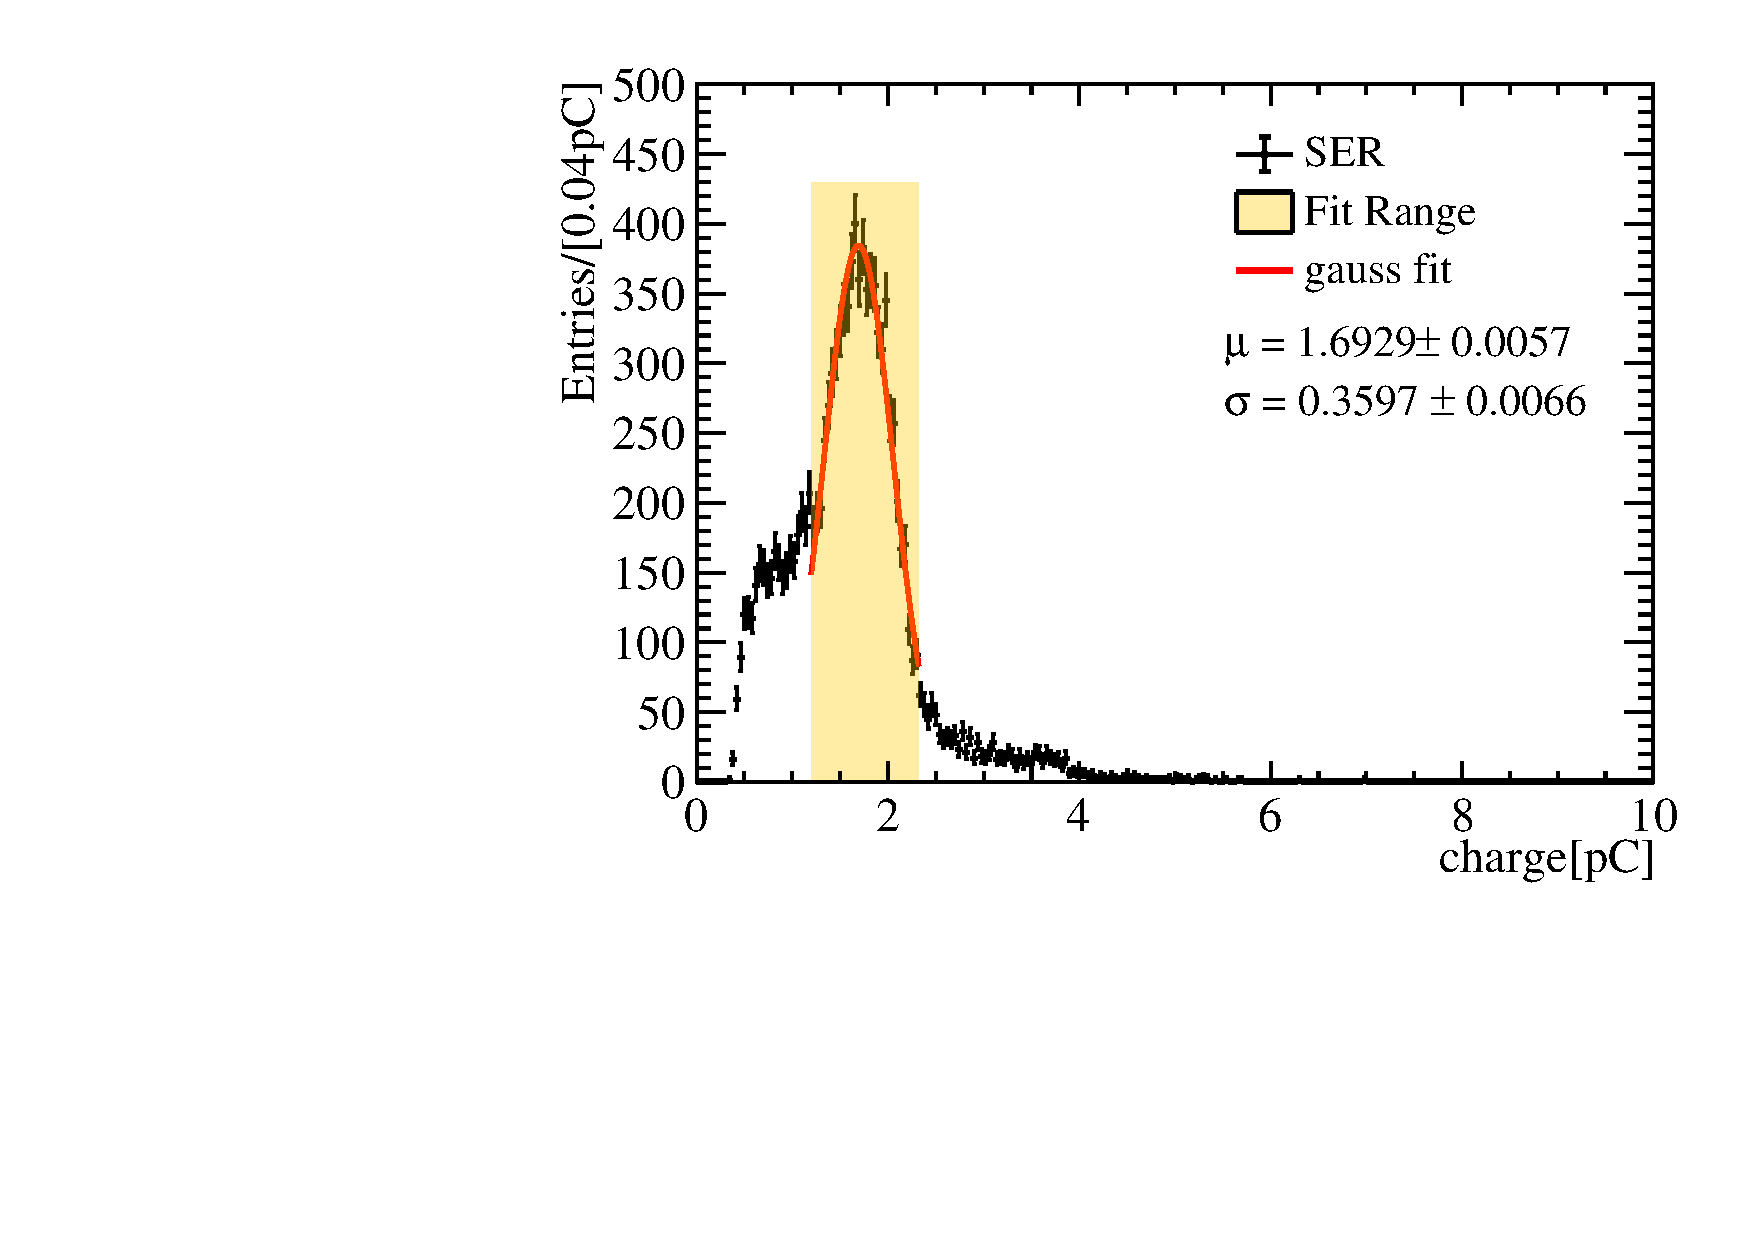
\includegraphics[width=\textwidth]{PMTRelated/GTmodel/fit_noald.pdf}
		\caption{}
		\label{fig:gain_noald}
	\end{subfigure}
	\hfill
	\begin{subfigure}[b]{0.48\textwidth}
		\centering
		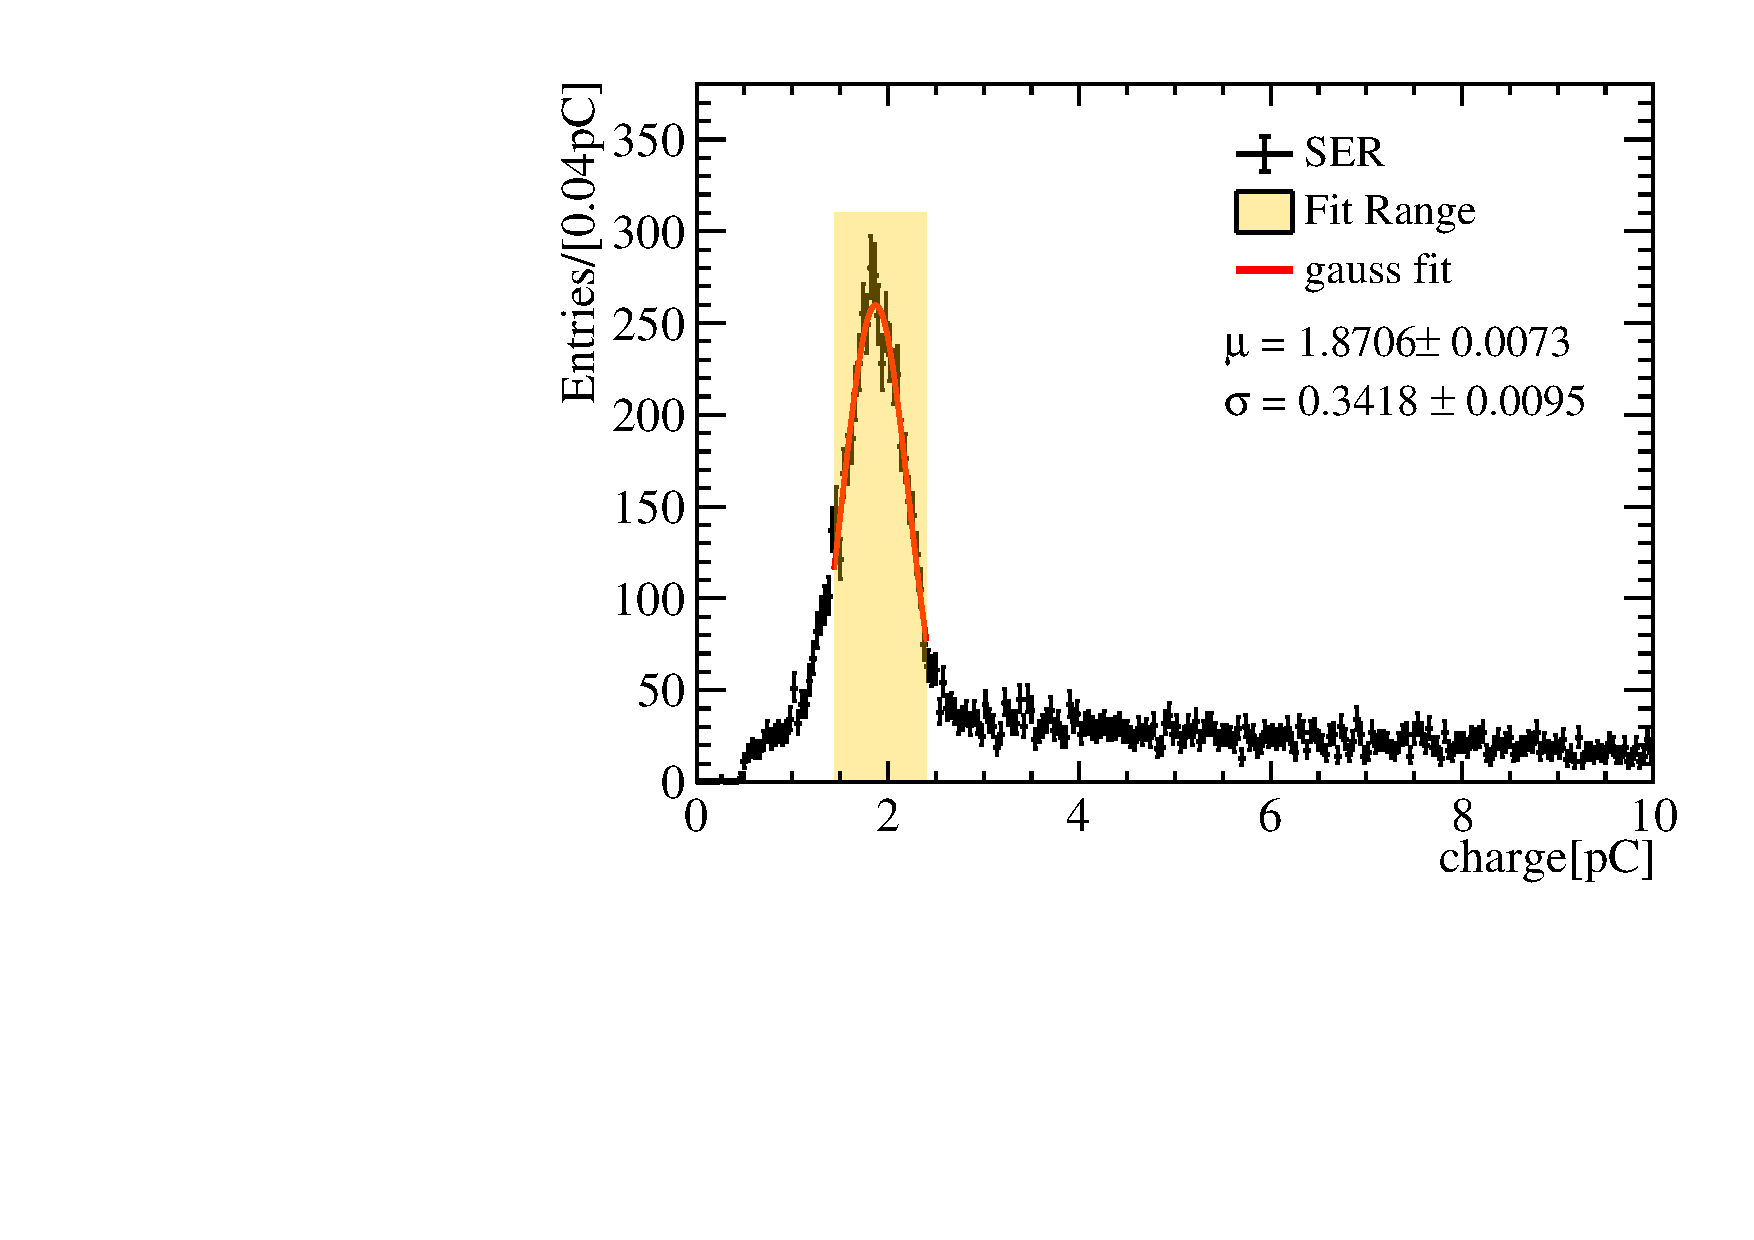
\includegraphics[width=\textwidth]{PMTRelated/GTmodel/fit_ald.pdf}
		\caption{}
		\label{fig:gain_ald}
	\end{subfigure}

	\caption{Fit of the charge spectrum of the MCP-PMT without \subref{fig:gain_noald} and with \subref{fig:gain_ald}
		\ce{Al2O3}-\ce{MgO} deposited on $\mathrm{M}1$.
		We observed that \subref{fig:gain_noald} does not exhibit jumbo charges.
		The yellow areas are incident energy-dependent intervals and
		the red lines are fitting results of the Gaussian functions in the intervals.
	}
	\label{fig:gain_fit}
\end{figure}

After fitting with Gaussians, we interpolate and extrapolate linearly to obtain the relations of $\mu(E_0)$ and $\sigma(E_0)$ in Fig.~\ref{fig:gaintest}.
The difference in the relations of MCP-PMTs with and without \ce{Al2O3}-\ce{MgO} deposited on $\mathrm{M}1$ comes from the influence of the charge contributed from the surface mode.
When \(E_0 < \SI{200}{eV}\), \(\mu(E_0)\) rapidly increases.
As \(E_0 > \SI{200}{eV}\), \(\mu(E_0)\) gradually stabilizes.
The $\sigma(E_0)$ is overall increasing similar to $\mu(E_0)$ but sees a drop around \SI{200}{eV}.
A similar trend of \(\mu(E_0)\) is reported by Yang~et~al.~\cite{2017MCP}.
In our case, the best relative resolution \(\sigma/\mu\) is at around \SI{600}{eV} and
Yang~et~al.'s results suggested \SI{200}{eV}.
Cao~et~al.\cite{cao_secondary_2021} found that the SEY of \ce{Al2O3}-\ce{MgO}
increases with the incident energy in 100--\SI{600}{eV}.
Even though the film structure and thickness we used are different,
we can still make a rough assessment that
the trend of $\sigma/\mu$ obtained here is reasonable,
considering the variation curves of the SEY of \ce{Al2O3} and \ce{MgO} with energy.
\begin{figure}[!ht]
	\centering
	\begin{subfigure}[b]{0.45\textwidth}
		\centering
		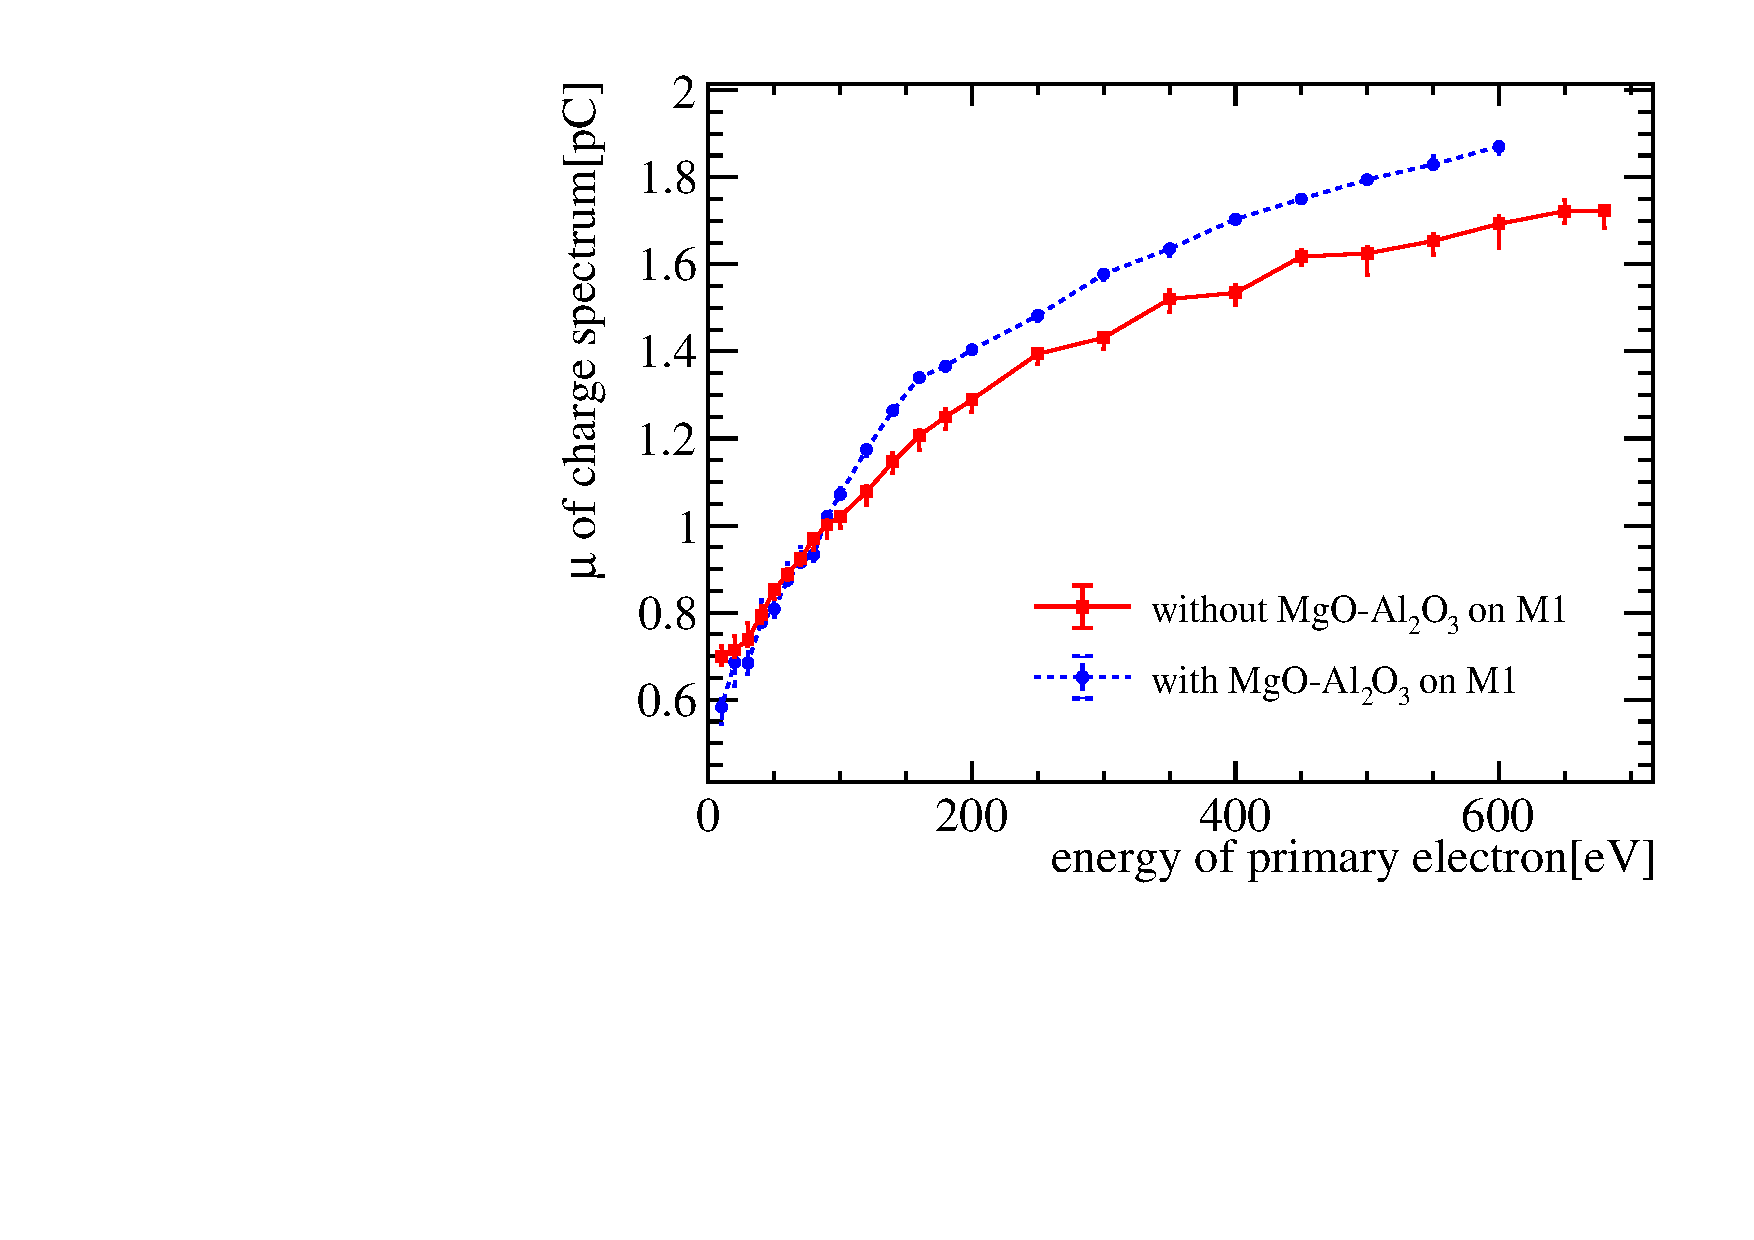
\includegraphics[width=\textwidth]{PMTRelated/GTmodel/gain_mu.pdf}
		\caption{}
		\label{fig:gain}
	\end{subfigure}%
	\begin{subfigure}[b]{0.45\textwidth}
		\centering
		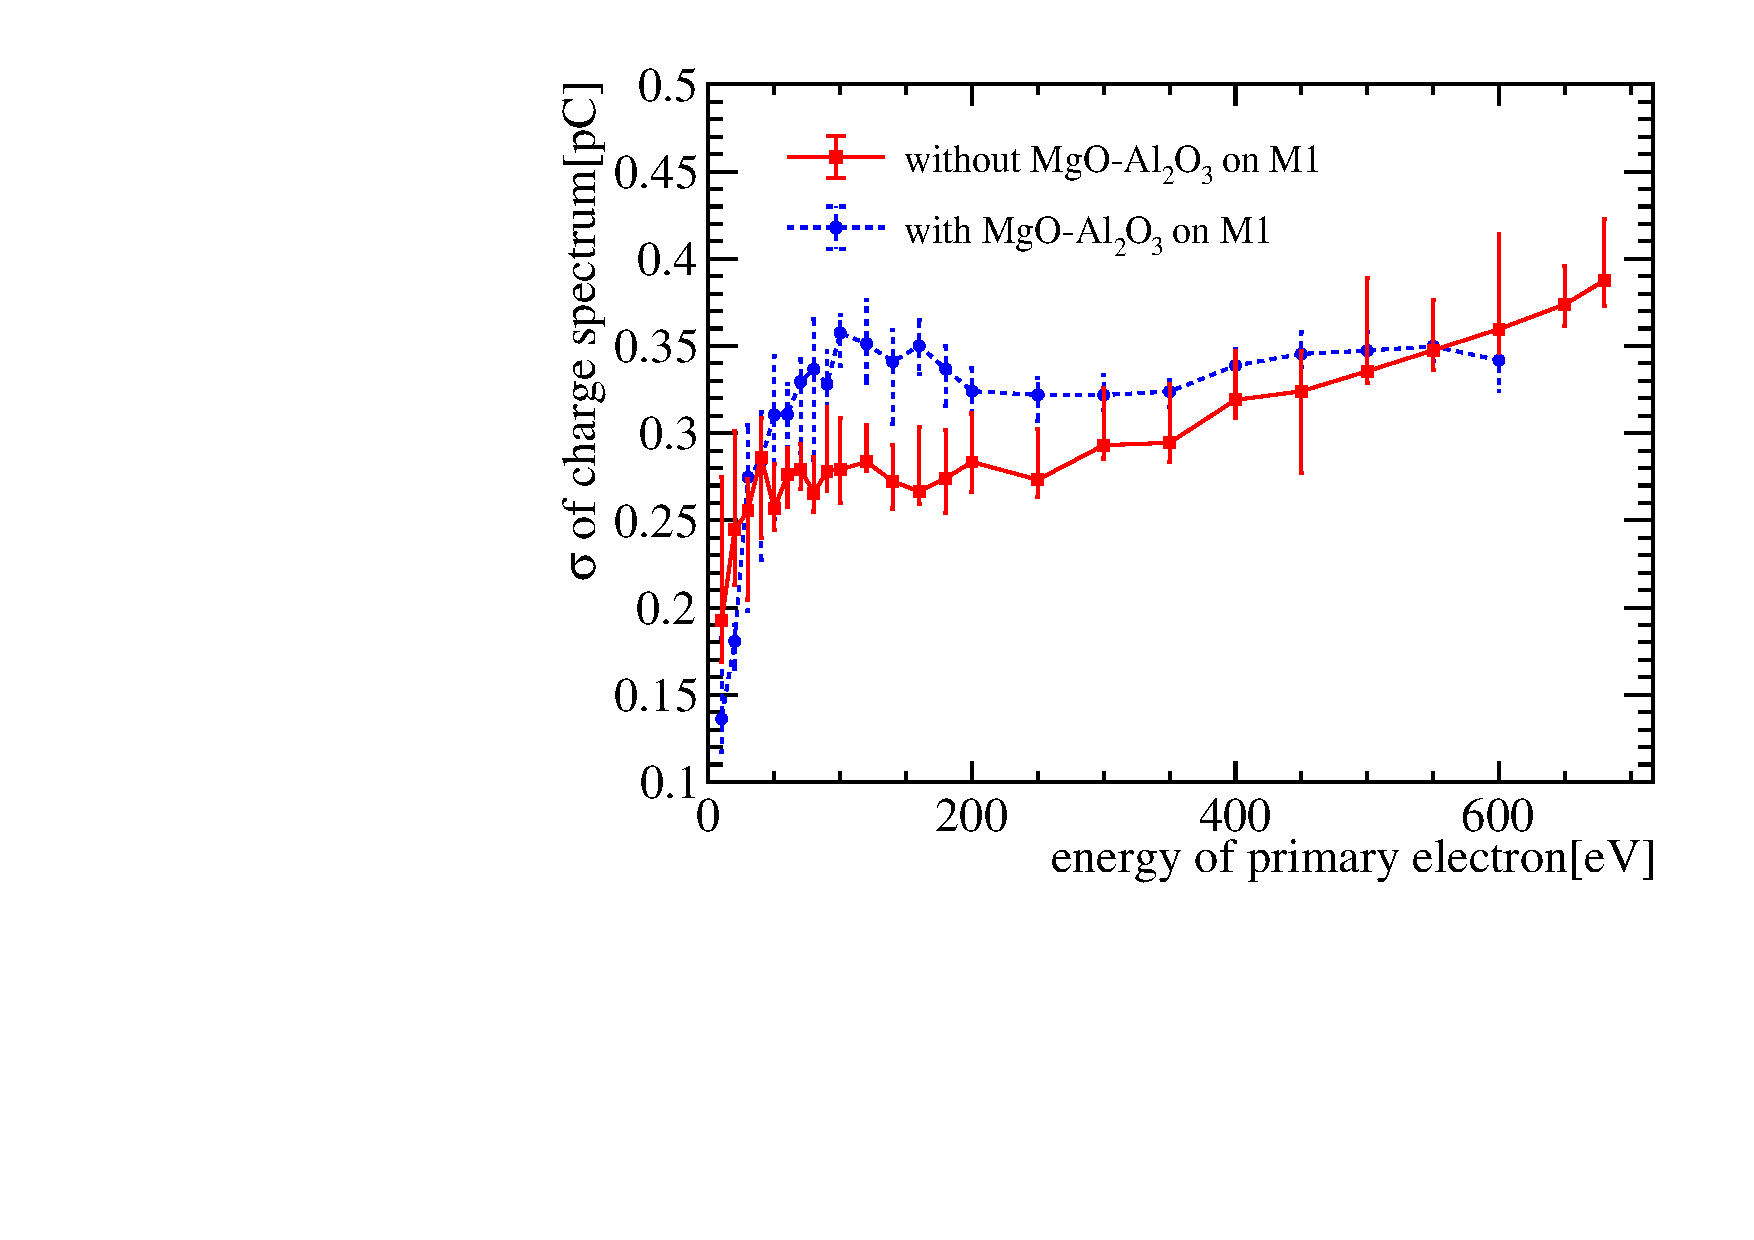
\includegraphics[width=\textwidth]{PMTRelated/GTmodel/gain_sigma.pdf}
		\caption{}
		\label{fig:sigma}
	\end{subfigure}
	\hfill
	\begin{subfigure}[b]{0.45\textwidth}
		\centering
		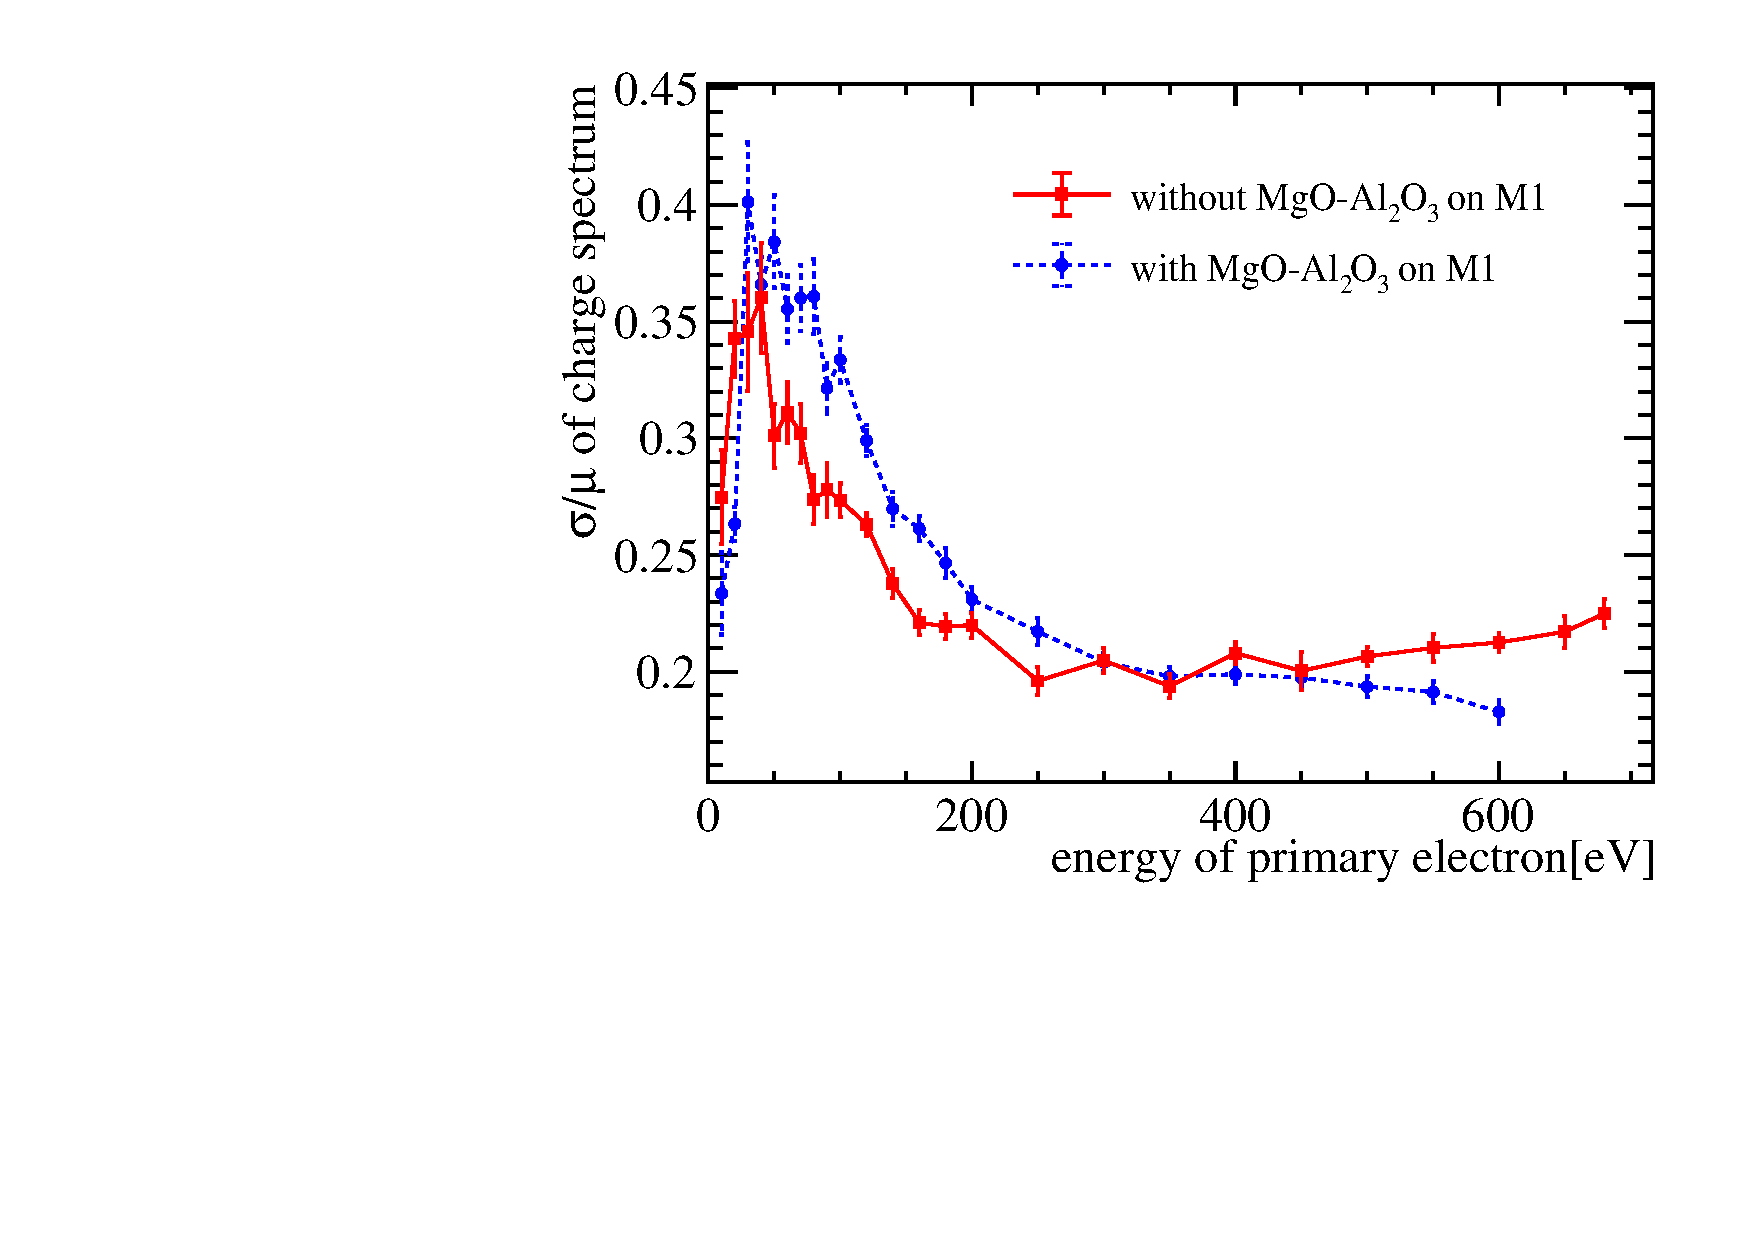
\includegraphics[width=\textwidth]{PMTRelated/GTmodel/gain_sigmamu.pdf}
		\caption{}
		\label{fig:sigmamu}
	\end{subfigure}
	\caption{\subref{fig:gain} The mean \(\mu\) increases as the incoming electron energy~$E_0$ increases.
		\subref{fig:sigma} The standard deviation \(\sigma\) changes with energy.
		The MCP-PMT with \ce{Al2O3}-\ce{MgO} deposited on $\mathrm{M}1$~(the red line) shows a similar variation trend to the one without~(the blue line).
		\subref{fig:sigmamu} The resolution $\sigma/\mu$ increases between 0-\SI{50}{eV}, decreases between 50-\SI{400}{eV},
		and after \SI{400}{eV}, there is a slight decrease for those with \ce{Al2O3}-\ce{MgO} deposited on $\mathrm{M}1$ ~(the blue line) and a slight increase for those without~(the red line).
	}
	\label{fig:gaintest}
\end{figure}

\subsubsection{Charge-Spectra Decomposition}\label{sec:convolution}
The Furman model in Sec.~\ref{subsec:fuman} predicts the energies of the secondaries.
Our voltage-division experiment in Sec.~\ref{sec:gain} measured the relationship between the
MCP gain and the incident energies of the electrons.
We follow the flowchart in Fig.~\ref{fig:process} to calculate the charge distribution by Monte Carlo.
In this study, we shone the laser at the apex of the photocathode hemisphere,
and the PEs hit M1 with an incident angle~$\theta_0=0^\circ$.
The complex amplification process in the channels is described by
the incident energy-dependent Gamma distributions $\varGamma(\alpha(E), \beta(E))$ described in Sec.~\ref{gammapossion}. The $\alpha(E)$ and $\beta(E)$ are estimated with the relations of $\mu(E)$ and $\sigma(E)$ of MCP-PMT without \ce{Al2O3}-\ce{MgO} coating on the input electrode, which eliminates the influence of the surface mode.
\begin{figure}[!ht]
	\centering
	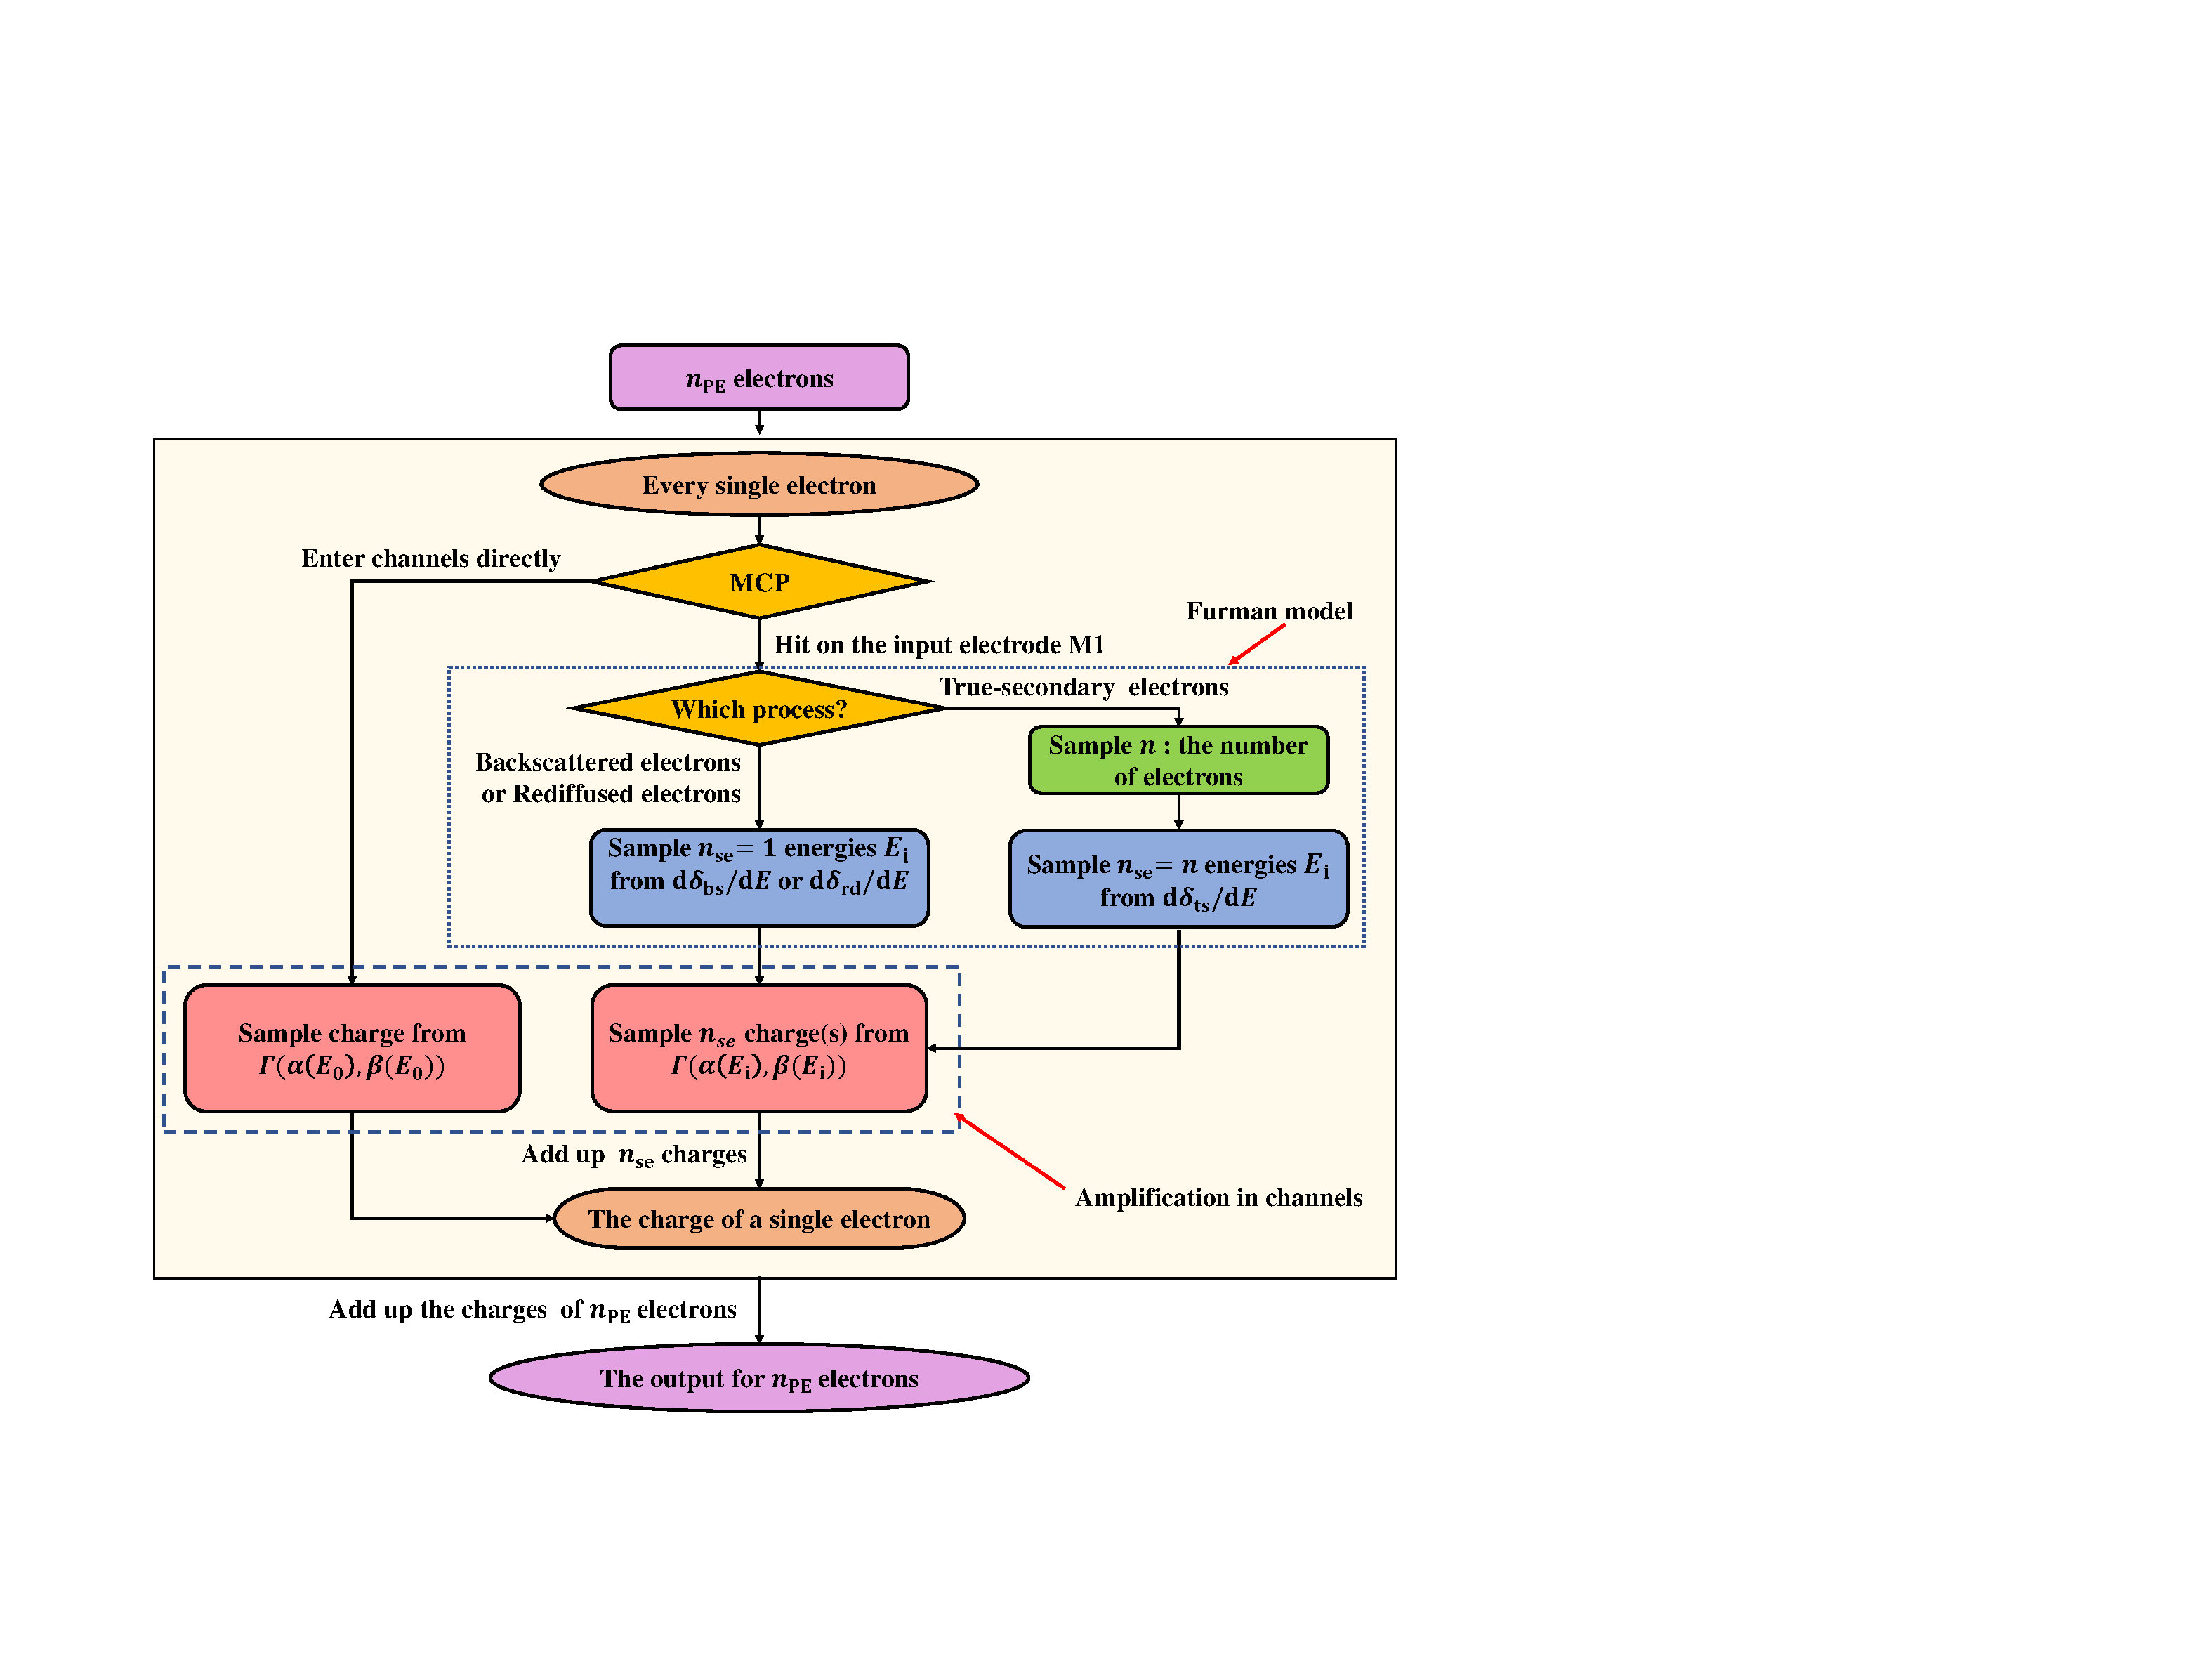
\includegraphics[width=\linewidth]{PMTRelated/GTmodel/process.pdf}
	\caption{The flowchart of Monte Carlo to compute the charge spectrum.
		The output charge consists of $n_\mathrm{PE}$ SER charges.
		The PEs in the channel mode enter channels directly, while PEs in the surface mode hit the input electrode.
		The energies of the $n_\mathrm{se}$ secondaries in the surface mode are sampled from the Furman model.
		The amplification in channels is modeled by the incident energy-dependent Gamma distribution.
	}
	\label{fig:process}
\end{figure}
Taking into account the light intensity, we repeatedly sample $n_{\mathrm{PE}}$ from the Poisson distribution
and sum up $n_{\mathrm{PE}}$ SER charges for the output to get a spectrum.

For sampling an SER charge, we assign the probabilities of the channel and surface
modes as $p$ and $1-p$ for a Bernoulli trial. The SER charge spectrum $f_{\text{MCP-PMT}}(Q)$ is
\begin{equation}
	\label{eq:convolution}
	f_{\text{MCP-PMT}}(Q) = p f_{\mathrm{ch}}(Q)+(1-p) f_{\mathrm{surf}}(Q)
\end{equation}
where $f_{\mathrm{ch}}(Q)$ and $f_{\mathrm{surf}}(Q)$ are the charge distributions of the channel and surface modes.
$f_{\mathrm{ch}}(Q)$ is set to \(f_\Gamma(Q; \alpha(E_0), \beta(E_0))\), with the incident energy being \SI{650}{eV}.
The factors \(\alpha(E_0), \beta(E_0)\) are converted from $\mu(E_0)$ and $\sigma(E_0)$ without \ce{Al2O3}-\ce{MgO} coating in Fig.~\ref{fig:gaintest}.

The \(f_{\mathrm{surf}}(Q)\) is divided into three components by the Furman model
corresponding to Eqs.~(\ref{eq:backscatter})--(\ref{eq:true}),
$f_{\mathrm{bs}}(Q)$ for the back-scattered electrons,
$f_{\mathrm{rd}}(Q)$ for the rediffused electrons,
and $f_{\mathrm{ts}}(Q)$ for the true-secondary electrons.
\begin{equation}
	\label{eq:surface_3}
	\begin{aligned}
		f_{\mathrm{surf}}(Q) & = p_{\mathrm{bs}} f_{\mathrm{bs}}(Q) + p_{\mathrm{rd}} f_{\mathrm{rd}}(Q) + (1- p_{\mathrm{bs}} - p_{\mathrm{rd}}) f_{\mathrm{ts}}(Q)                     \\
		                     & = \delta_{\mathrm{bs}} f_{\mathrm{bs}}(Q) + \delta_{\mathrm{rd}} f_{\mathrm{rd}}(Q) + (1- \delta_{\mathrm{bs}} - \delta_{\mathrm{rd}}) f_{\mathrm{ts}}(Q) \\
	\end{aligned}
\end{equation}
where $p_{\mathrm{bs}}$ and $p_{\mathrm{rd}}$ are the mixture ratios
determined by the composition and thickness of surface emissive material
that varies among the PMTs.  Furman and Pivi~\cite{2002Probabilistic} assume that
only one electron is emitted in back-scattered mode and rediffused mode
so that \(\delta_{\mathrm{bs}} = p_{\mathrm{bs}}\) and \(\delta_{\mathrm{rd}} = p_{\mathrm{rd}}\).
In the calculation, we specify $\delta_{\mathrm{rd}}=0.09$ and $\delta_{\mathrm{bs}}=0.01$.
The energy of the back-scattered electron is nearly equal to that of the PEs in the channel mode,
and so is the MCP gain for them.
The energy of the rediffused electron
is lower -- from \SIrange{100}{600}{eV}, causing the charge after MCP multiplication
to be slightly smaller thanks to the relatively slow increase of gain in that range in Fig.~\ref{fig:gain}.
Either contributes a single electron and is practically indistinguishable from
the channel mode in the charge spectra. Such a degeneracy is summarized in Eq.~\eqref{eq:gammaTweedie}:
\begin{equation}
	\label{eq:gammaTweedie}
	\begin{aligned}
		f_{\text{MCP-PMT}}(Q) & = p f_{\mathrm{ch}}(Q) + (1-p) f_{\mathrm{surf}}(Q)                                                                                                                                    \\
		                      & = p f_{\mathrm{ch}}(Q)+(1-p) [\delta_{\mathrm{bs}} f_{\mathrm{bs}}(Q) + \delta_{\mathrm{rd}} f_{\mathrm{rd}}(Q) + (1- \delta_{\mathrm{bs}} - \delta_{\mathrm{rd}}) f_{\mathrm{ts}}(Q)] \\
		                      & = [p + (1-p)(\delta_{\mathrm{bs}} + \delta_{\mathrm{rd}})] f_{\mathrm{ch}}(Q) + (1-p)(1-\delta_{\mathrm{bs}} - \delta_{\mathrm{rd}})f_{\mathrm{ts}}(Q)
	\end{aligned}
\end{equation}
where the spectra $f_{\mathrm{ch}}(Q)$, $f_{\mathrm{rd}}(Q)$ and $f_{\mathrm{bs}}(Q)$ are
merged into $f_{\mathrm{ch}}(Q)$.

Nevertheless, Eq.~(\ref{eq:gammaTweedie}) is incomplete.
We should consider the case when the secondaries hit the MCP surface again.
The round trip does not inject extra energy.
A back-scattered or rediffused secondary gets amplified essentially in the same way
as a primary PE, while a true-secondary electron has too low energy to multiply again.
Therefore, \(p_0\), the net contribution to \(f_{\mathrm{ch}}(Q)\), is a geometric series
\begin{equation}
	\label{eq:p0}
	p_0 = p \sum_{{i}=0}^\infty [(1-p) (\delta_{\mathrm{bs}} + \delta_{\mathrm{rd}})]^{i} = \frac{p}{1 - (1-p) (\delta_{\mathrm{bs}} + \delta_{\mathrm{rd}})}
\end{equation}
and \(f_{\mathrm{ts}}(Q)\) gets \(\frac{(1-p)(1-\delta_{\mathrm{bs}} - \delta_{\mathrm{rd}})}{1 - (1-p) (\delta_{\mathrm{bs}} + \delta_{\mathrm{rd}})}\) or \(1-p_0\).
Eq.~(\ref{eq:gammaTweedie}) is remarkably reduced to
\begin{equation}
	\label{eq:1}
	f_{\text{MCP-PMT}}(Q) = p_0 f_{\mathrm{ch}}(Q) + (1-p_0) f_{\mathrm{ts}}(Q).
\end{equation}

In the case of the true-secondary electrons, their count $n$ follows a Poissonian. The sum of the sampled $n$ charges
serves as the output \(Q_{\mathrm{ts}}\),
\begin{equation}
	\label{eq:ts_all}
	\begin{aligned}
		 & Q_{\mathrm{ts}} = \sum_{i=1}^{n} Q_{i}            \\
		 & n \sim \mathrm{\pi}(\delta_{\mathrm{ts}}')        \\
		 & Q_{i} \sim \varGamma[\alpha(E_{i}), \beta(E_{i})] \\
	\end{aligned}
\end{equation}
where \(E_{i}\) are sampled from Eq.~(\ref{eq:true}).
$\alpha(E_{i})$ and $\beta(E_{i})$ are converted from
\(\mu(E_{i})\) and \(\sigma(E_{i})\) of Fig.~\ref{fig:gaintest}.
For completeness, \(\delta_\mathrm{ts} = (1-\delta_{\mathrm{bs}} - \delta_{\mathrm{rd}})\delta_{\mathrm{ts}}'\)
is the electric-current ratio of the true-secondary electrons to that of the primary.

The charge spectra of different $n$ are shown in Fig.~\ref{fig:true_n}.
Due to the lower energies of the secondaries, their charges are smaller.
It is challenging to distinguish each charge formed at the anode,
as multiple secondary electrons enter the MCP channels simultaneously.
Bigger $n$ results in a larger charge.

\begin{figure}[!htbp]
	\begin{subfigure}{0.47\linewidth}
		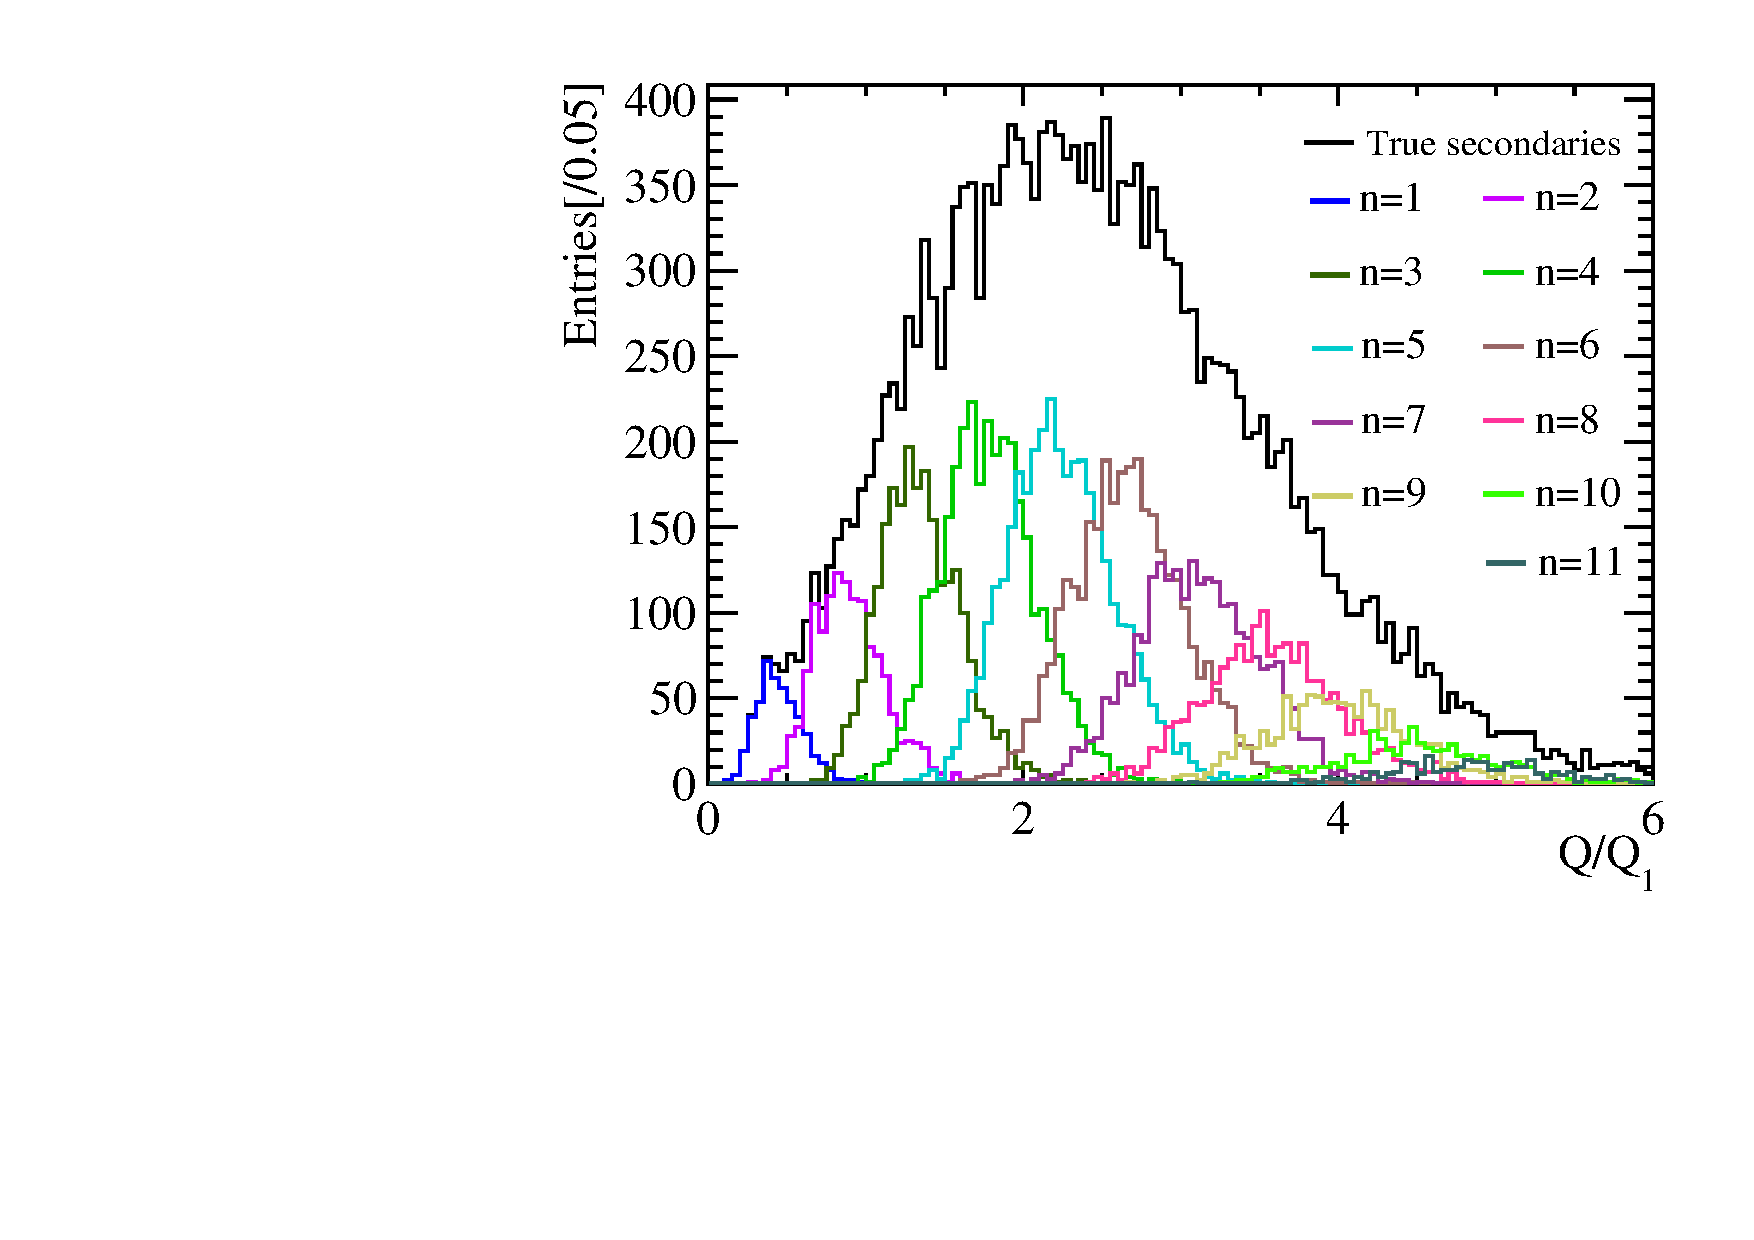
\includegraphics[width=\textwidth]{PMTRelated/GTmodel/true_all.pdf}
		\caption{}
		\label{fig:true_n}
	\end{subfigure}
	\hfill
	\begin{subfigure}{0.47\linewidth}
		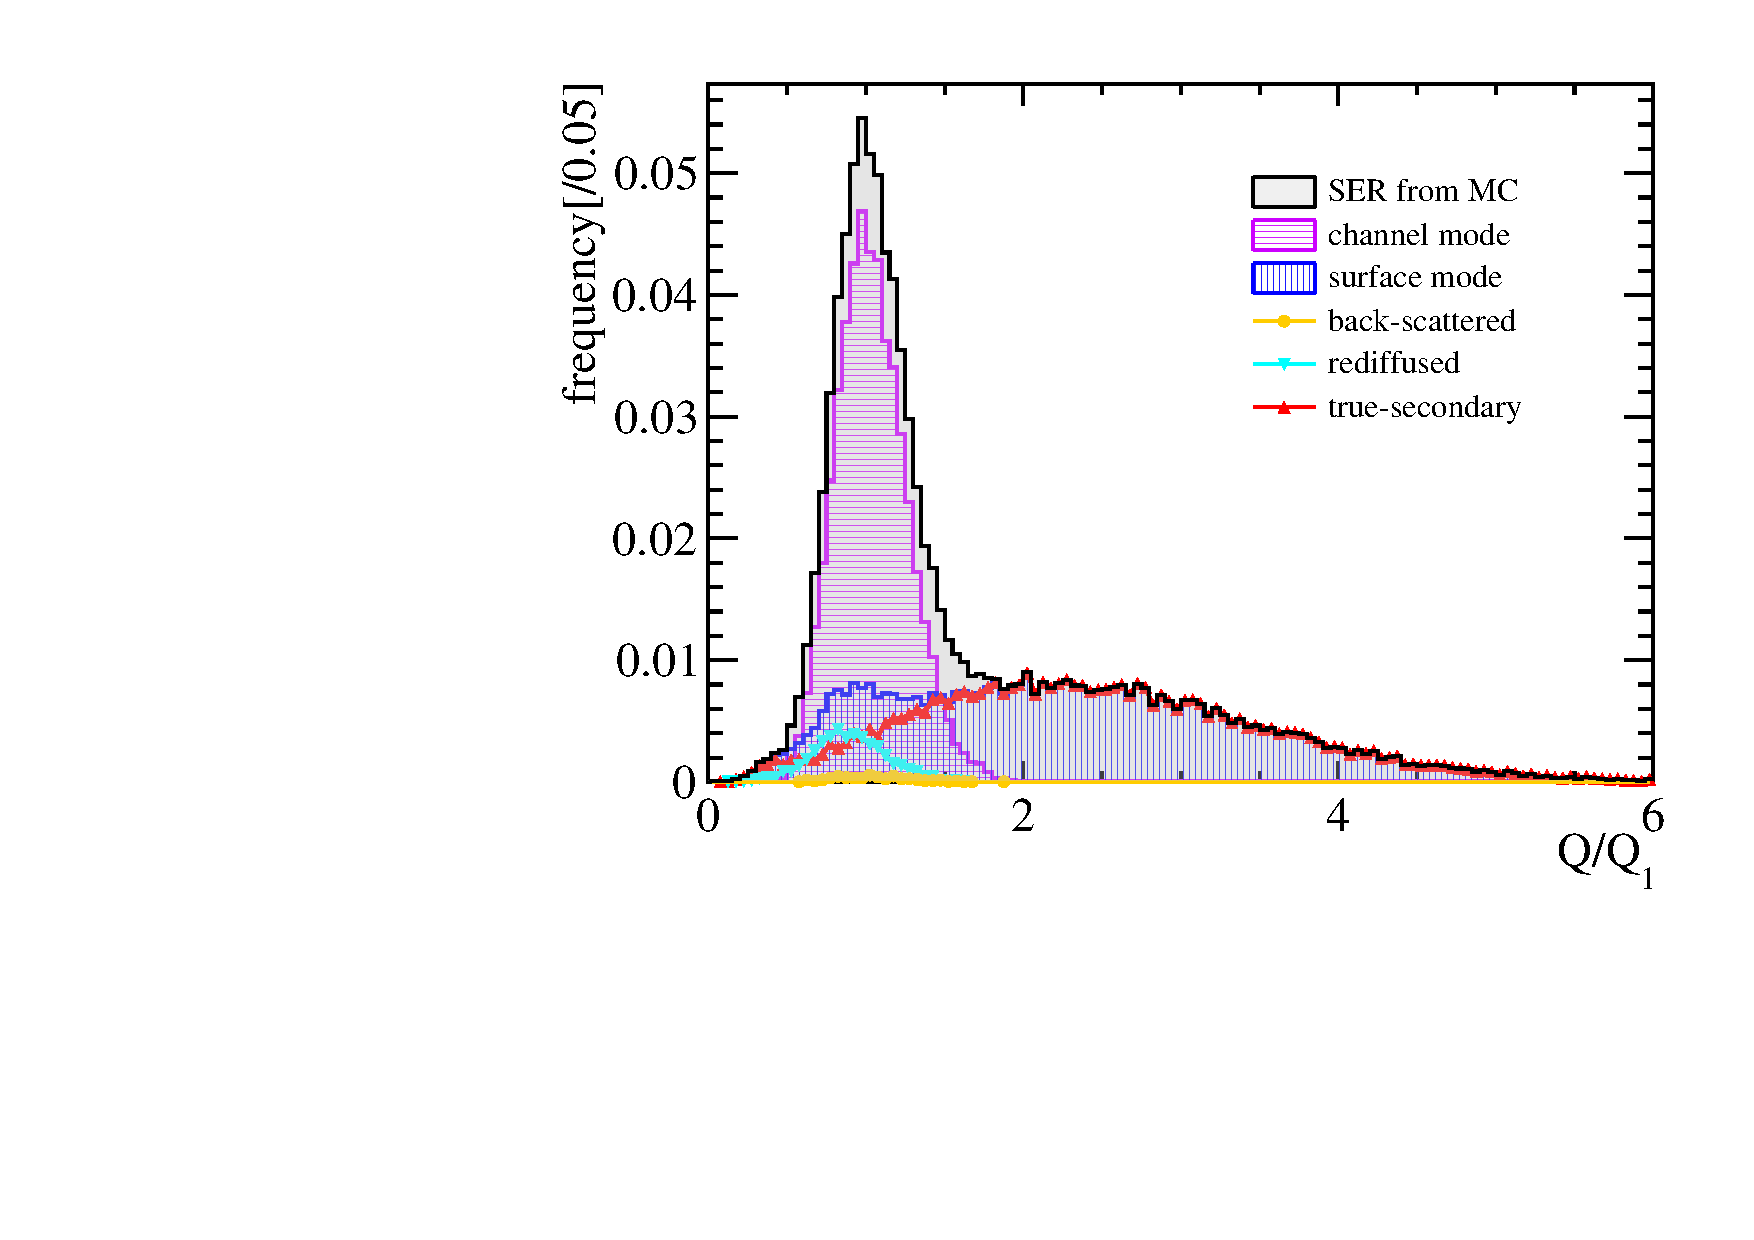
\includegraphics[width=\textwidth]{PMTRelated/GTmodel/allmode.pdf}
		\caption{}
		\label{fig:allmode}
	\end{subfigure}
	\caption{\subref{fig:true_n}: The charge distribution of the true-secondary electrons mode
		in the MC calculation when $\delta_{\mathrm{ts}}'=5.5$ and $p_0=0.55$.
		The black histogram gives the sum of all the distributions.
		\subref{fig:allmode}: The charge distribution formed in the channel mode is concentrated around the peak,
		while the tail portion is mainly generated by the true-secondary electrons in the surface mode.}
\end{figure}

A typical decomposition of the SER charge spectra is shown in Fig.~\ref{fig:allmode}.
The jumbo charges, also known as the ``long tail'', are contributed by the true secondaries
from the surface mode.

\subsection{Parameter Extraction from Data}\label{subsec:chitest}
It is evident from Eq.~(\ref{eq:1}) and (\ref{eq:ts_all}) that $\delta_{\mathrm{ts}}'$ and \(p_0\)
significantly impact the SER charge distribution, demonstrated in Fig.~\ref{fig:tsp}.  We use
the MCP-PMT test data by Zhang~et~al.~\cite{Zhang:2023ued} to determine the two parameters.
\begin{figure}[!htbp]
	\centering
	\begin{subfigure}{0.47\textwidth}
		\centering
		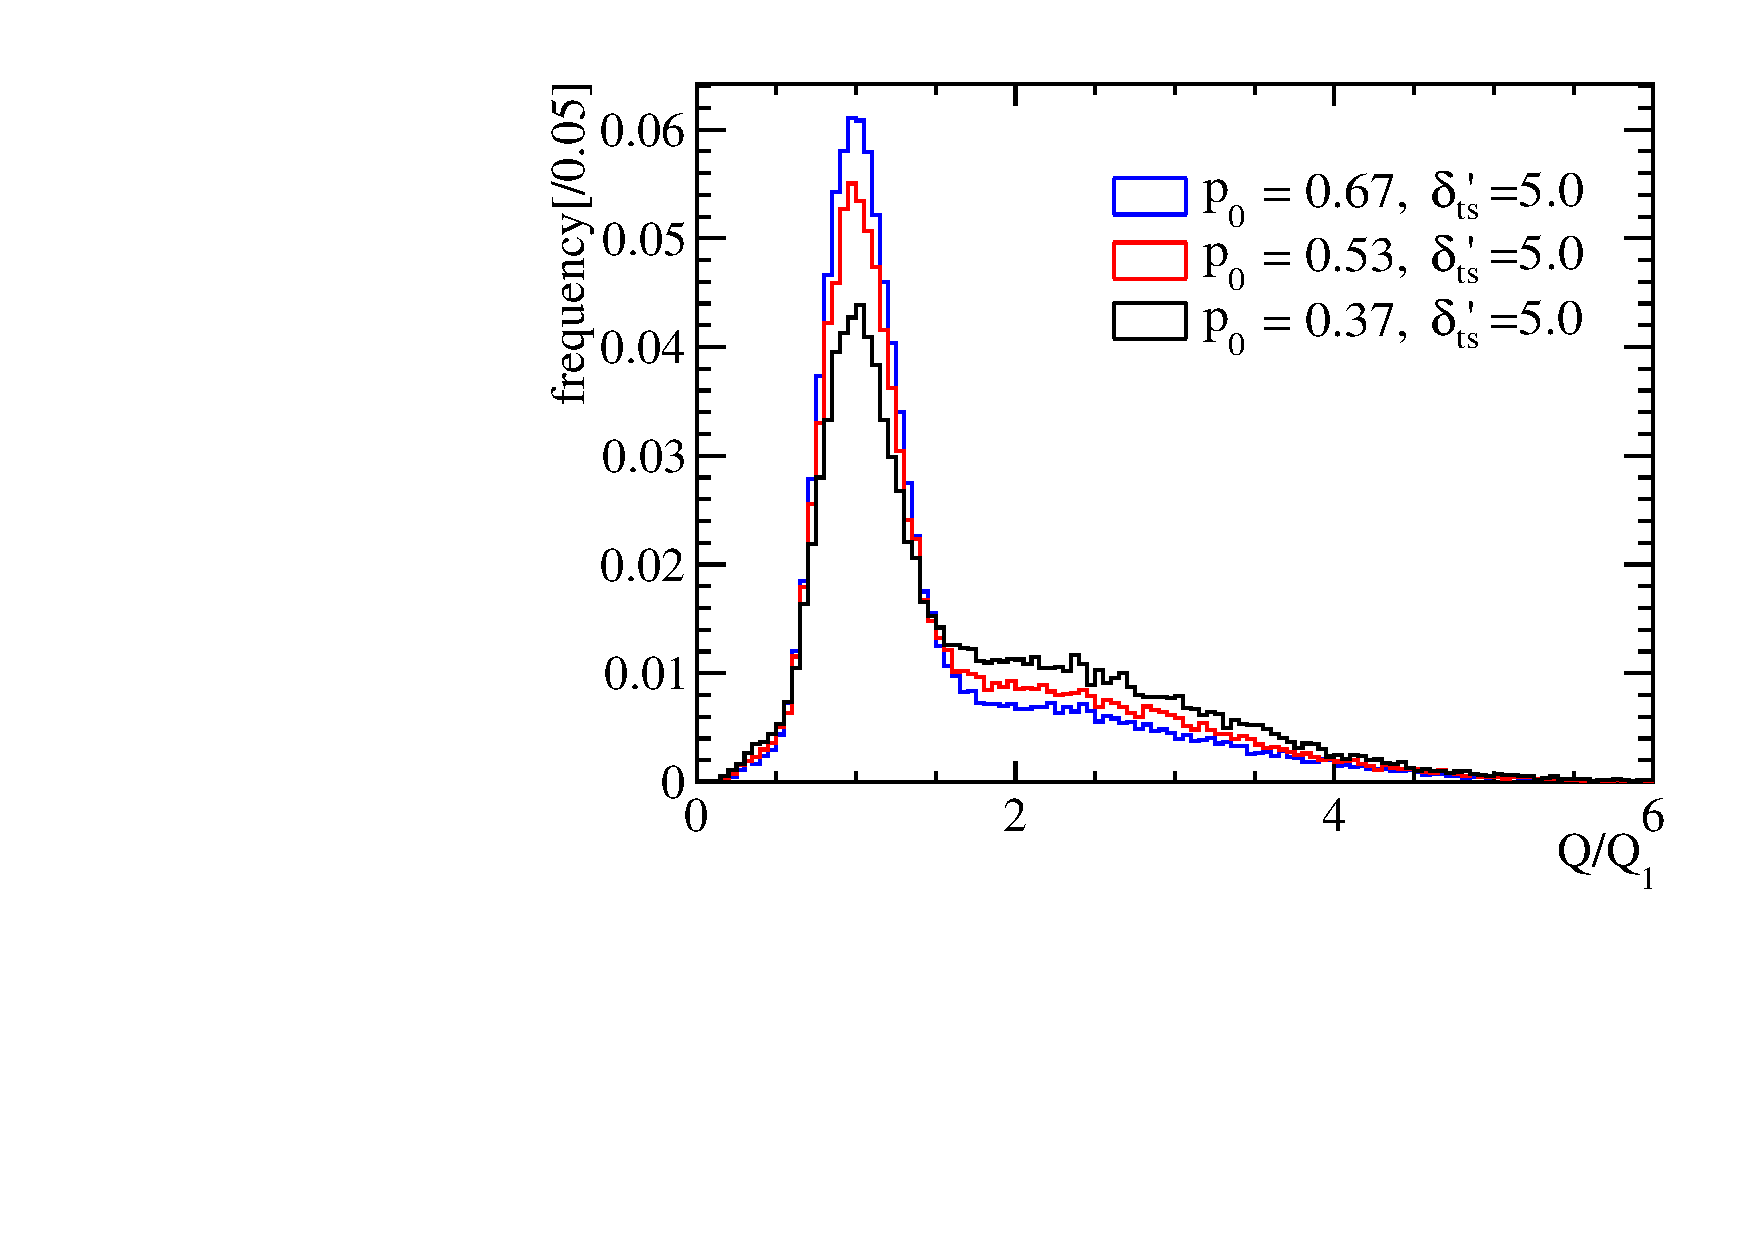
\includegraphics[width=\linewidth]{PMTRelated/GTmodel/p.pdf}
		\caption{}
		\label{fig:p}
	\end{subfigure}
	\hfill
	\begin{subfigure}{0.47\textwidth}
		\centering
		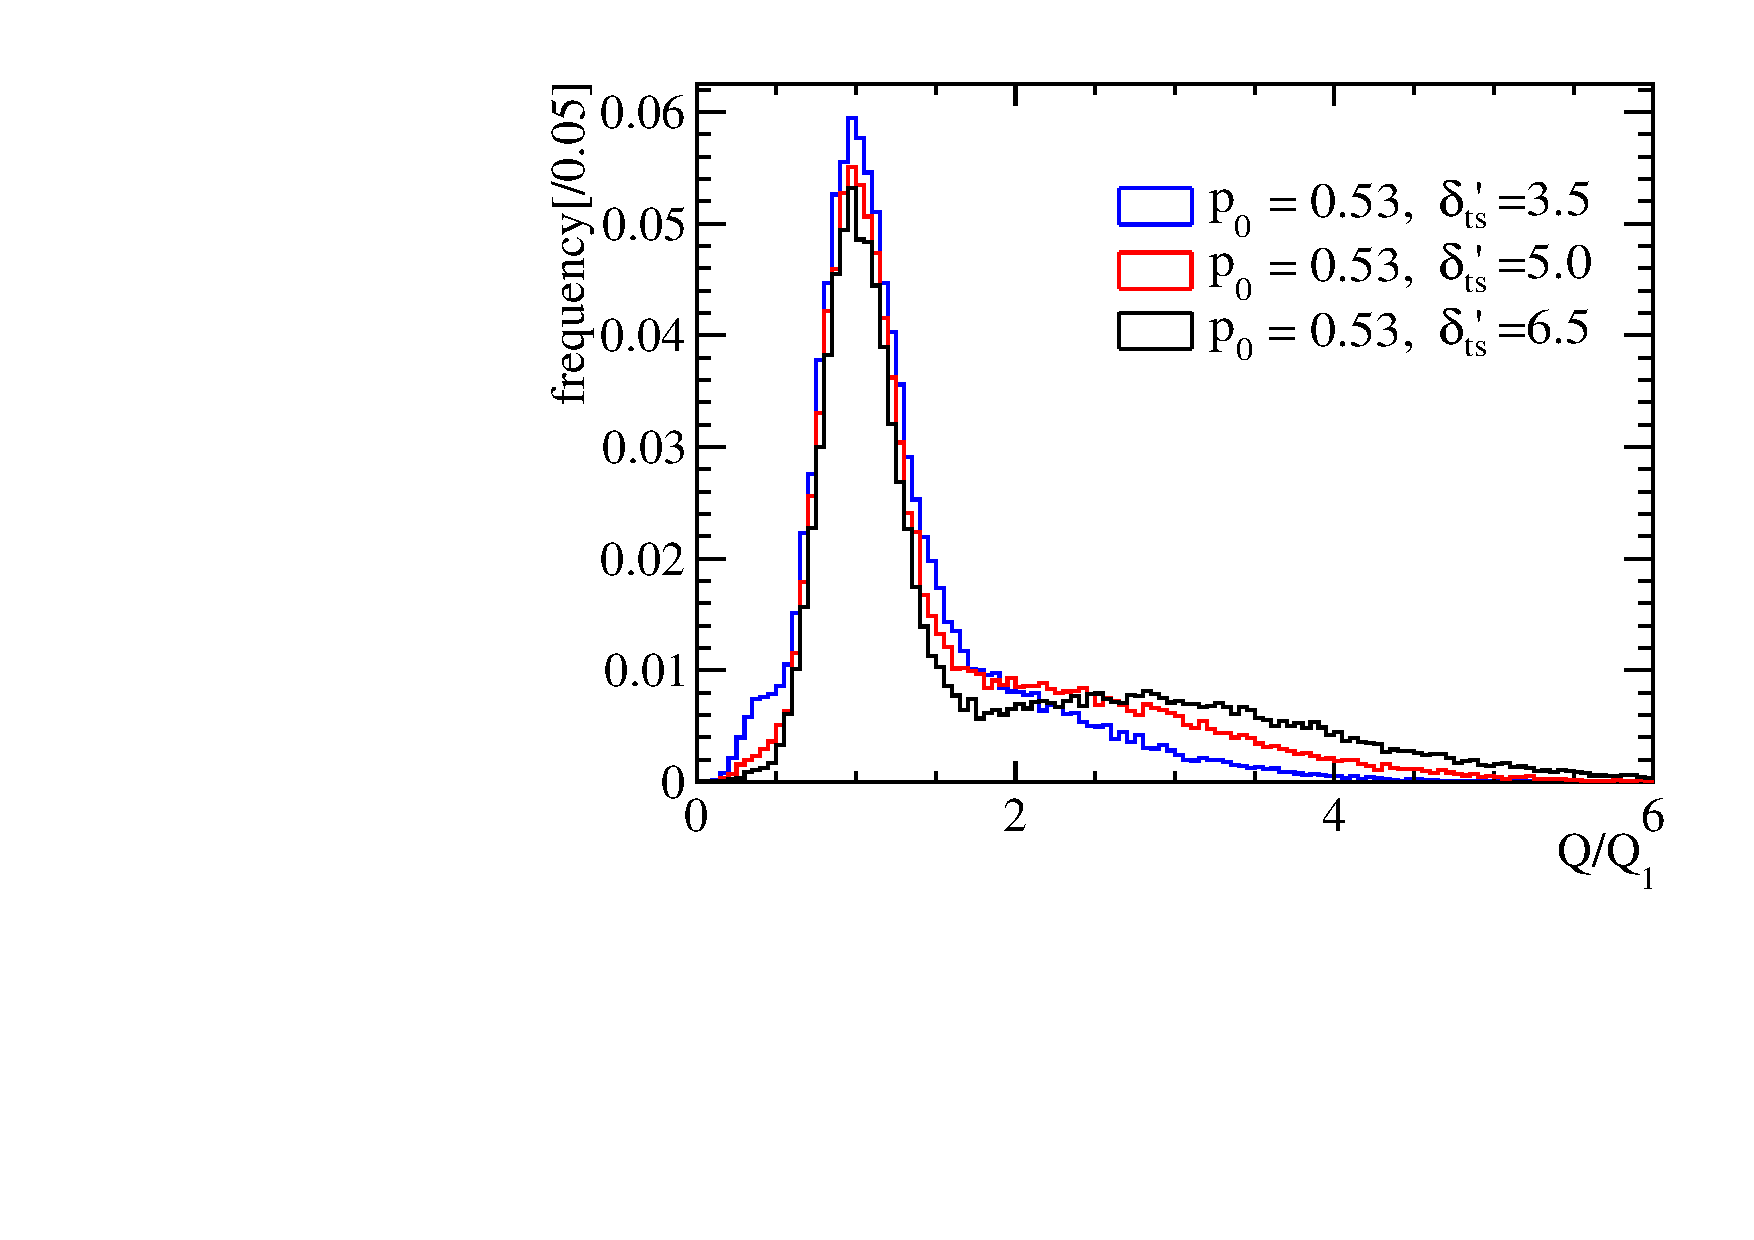
\includegraphics[width=\linewidth]{PMTRelated/GTmodel/ts.pdf}
		\caption{}
		\label{fig:ts}
	\end{subfigure}
	\caption{$\delta_{\mathrm{ts}}'$ and $p_0$ influence the shape of SER charge spectrum from MC.
		As $\delta_{\mathrm{ts}}'$ increases, the region of the tail becomes more prolonged.
		As $p_0$ increases, the height of the principal peak region increases, and the tail becomes narrower.
	}
	\label{fig:tsp}
\end{figure}

Between each pair of predicted and measured charge distributions, we perform a chi-square test.
These two histograms are divided into $r$ bins using the same binning method.
The entries in the \(i\)-th bin are $n_i$ and $m_{i}$, adding up to
$N = \sum_{{i}=1}^{r}n_{i}$ and $M = \sum_{{i}=1}^{r}m_{i}$.
The chi-square test indicates the similarity between two histograms~\cite{2006Comparison},
\begin{equation}
	\label{eq:chi}
	\chi^2_{r-1}=\sum_{{i}=1}^r \frac{\left(n_{i}-N \hat{k}_{i}\right)^2}{N \hat{k}_{i}}+\sum_{{i}=1}^r
	\frac{\left(m_{i}-M \hat{k}_{i}\right)^2}{M \hat{k}_{i}}=\frac{1}{M N} \sum_{{i}=1}^r
	\frac{\left(M n_{i}-N m_{i}\right)^2}{n_{i}+m_{i}}
\end{equation}
where \(\hat{k}_{i}=\frac{n_{i}+m_{i}}{N+M}\).

The \(\chi^2_{r-1}\) are scanned in the $(p_0,\delta_{\mathrm{ts}}')$ grid, with an example in Fig.~\ref{fig:cour}.
We use a linear model~\cite{Gelman_Hill_2006} to smooth the approximate parabolic relationship
between the \(\chi^2_{r-1}\) and $(p_0, \delta_{\mathrm{ts}}')$,
then extract the $(\hat{p}_0, \hat{\delta}_{\mathrm{ts}}')$ that minimizes \(\chi^2_{r-1}\) with
intervals at \SI{68.3}{\percent} confidence levels~\cite{cowan1997statistical}.

\begin{figure}[!htbp]
	\centering
	\begin{subfigure}{0.47\textwidth}
		\centering
		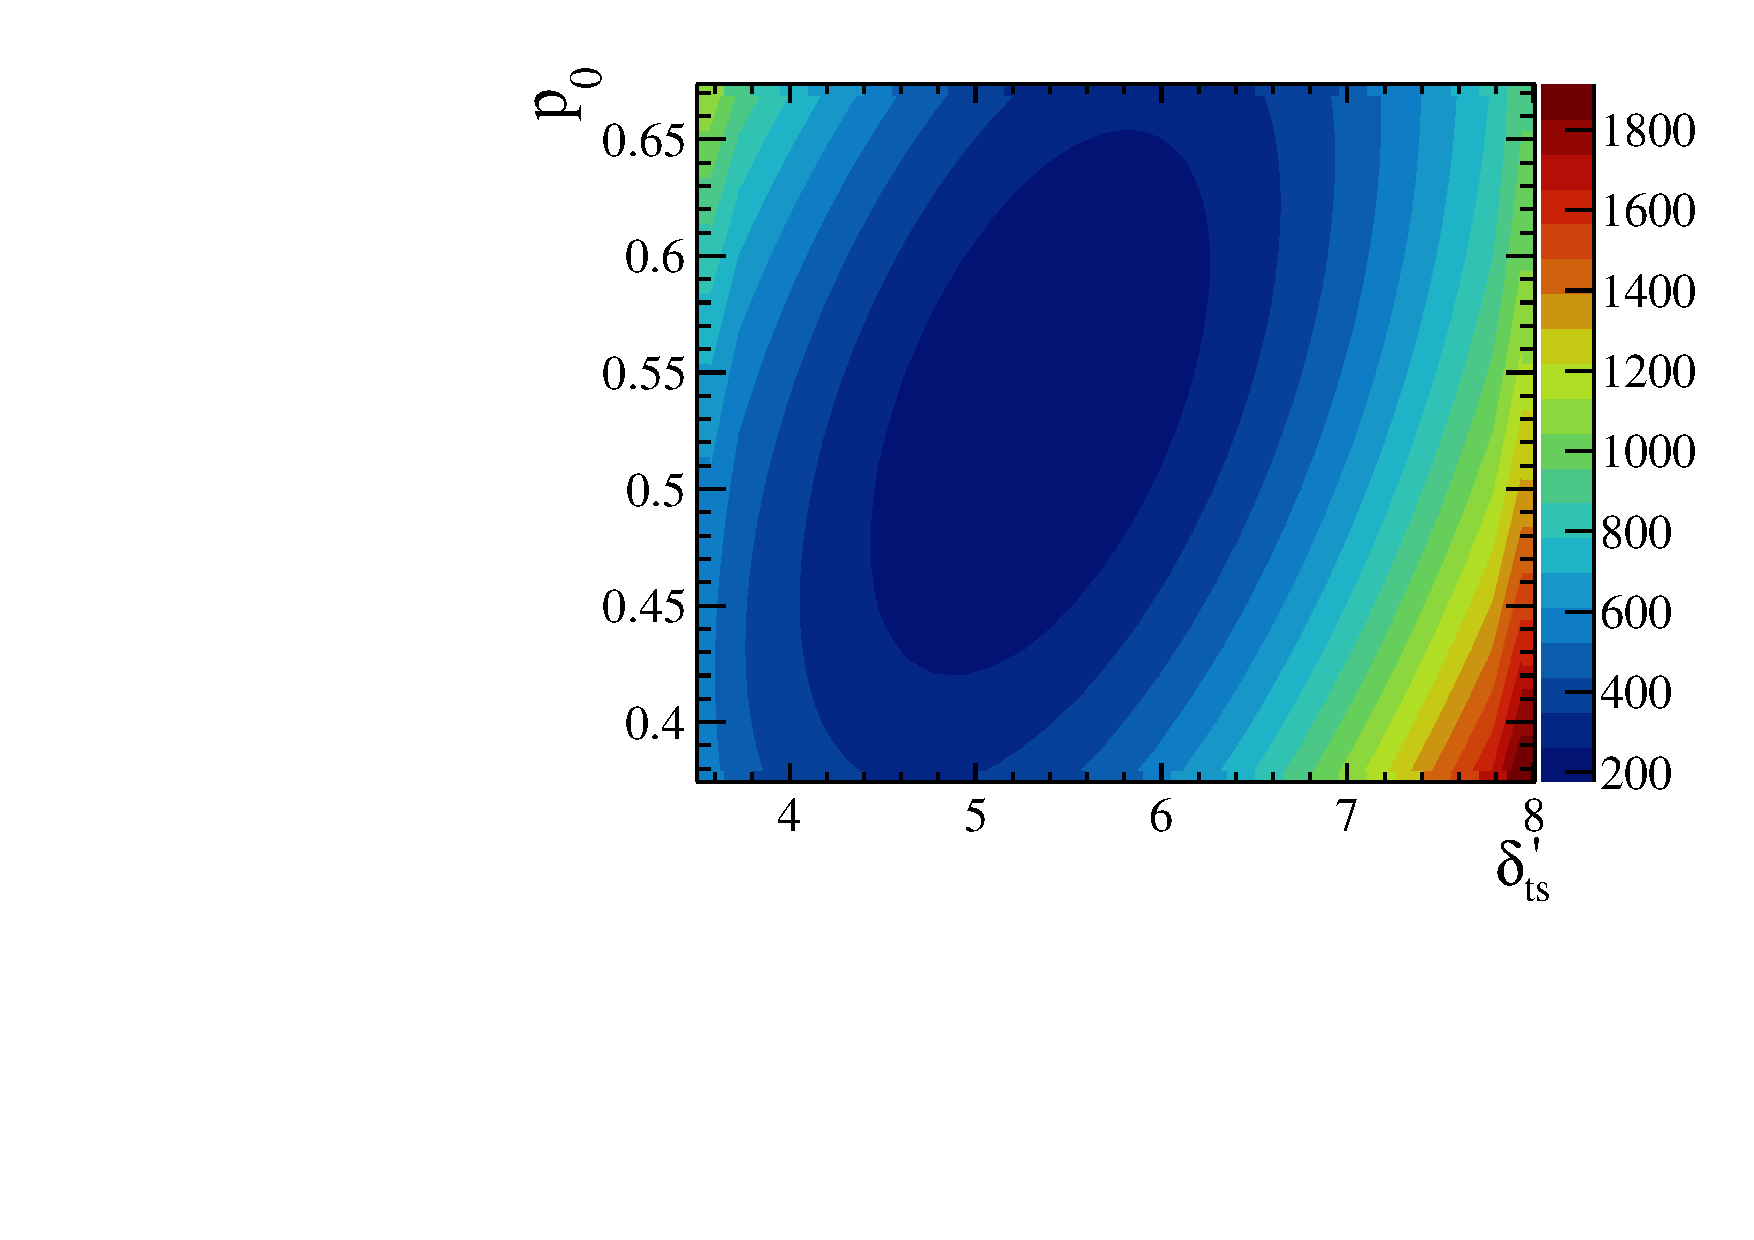
\includegraphics[width=\linewidth]{PMTRelated/GTmodel/cour.pdf}
		\caption{}
		\label{fig:cour}
	\end{subfigure}
	\hfill
	\begin{subfigure}{0.47\textwidth}
		\centering
		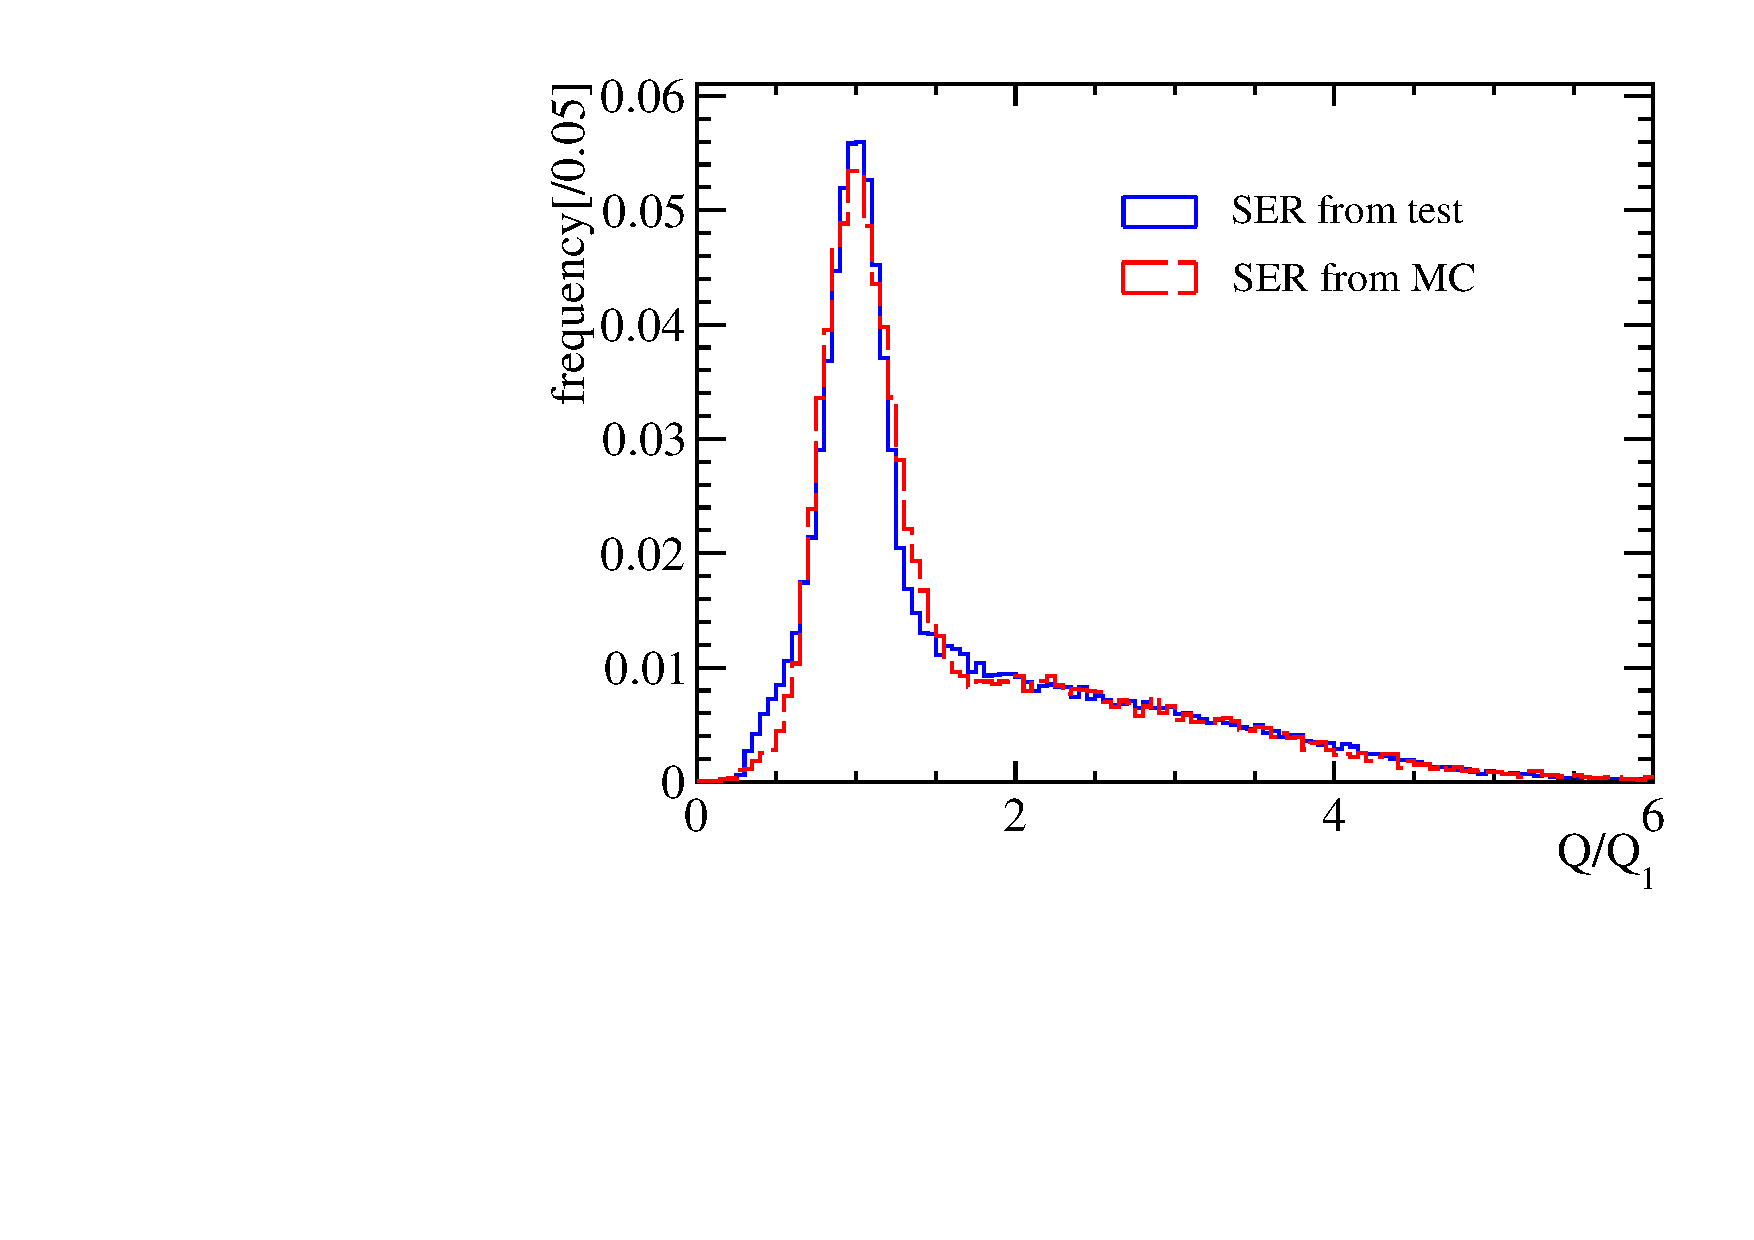
\includegraphics[width=\linewidth]{PMTRelated/GTmodel/hist.pdf}
		\caption{}
		\label{fig:hist}
	\end{subfigure}
	\caption{The plot~\subref{fig:cour} is the contour plot of the chi-square test, with $p_0$ and $\delta_{\mathrm{ts}}'$ as parameters
		and the chi-square values as the height.
		The plot~\subref{fig:hist} is an example of the MC histogram~(the red line) and the histogram from test~(the blue line).
	}
	\label{fig:chi}
\end{figure}

The $\hat{\delta}_{\mathrm{ts}}'$ vs. $\hat{p}_0$ scatter plot
of 9 MCP-PMTs in Fig.~\ref{fig:true_p} does not indicate a strong correlation.
They are determined by independent manufacturing stages.
On average, $\delta_{\mathrm{ts}}'$ is 5.979 and $p_0$ is 0.5341. % rd=0.09,bs=0.01
The PEs of the channel, back-scattered, and rediffused surface modes account for \SI{53.41}{\percent}.
They constitute the peak. Each of the rest hits the surface
to induce 5.979 true-secondary electrons on average.

\begin{figure}[!htbp]
	\centering
	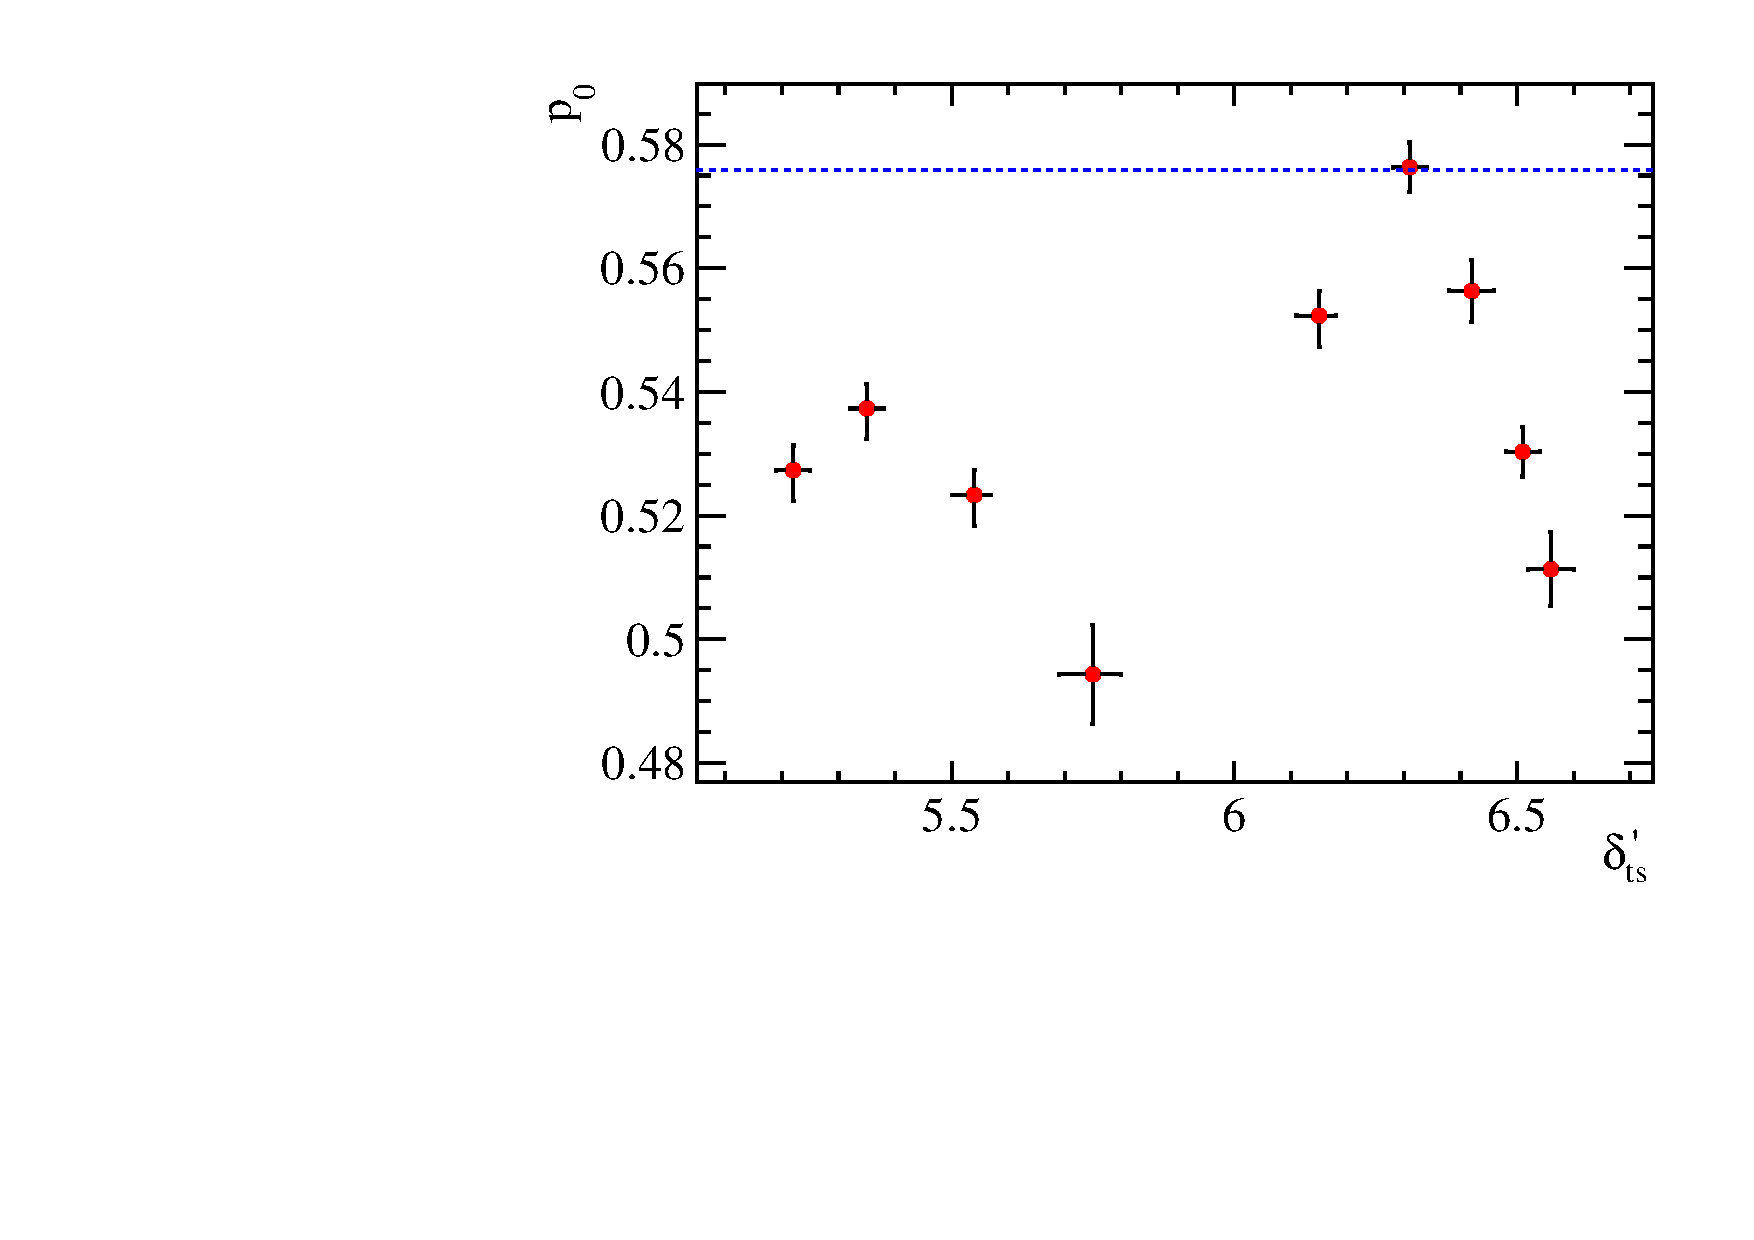
\includegraphics[width=0.6\textwidth]{PMTRelated/GTmodel/true_p.pdf}
	\caption{When convolving with 9 MCP-PMTs,
		the distribution of $\delta_{\mathrm{ts}}'$ and $p_0$ at the minimum chi-square
		occurs. The blue dashed line shows the expected $\hat{p}_0$ estimated from~\cite{chen2018photoelectron}.}
	\label{fig:true_p}
\end{figure}

To compare our measurement to previous studies, we convert \(\delta_\text{ts}'\)
to the SEY \(\delta\)
\begin{equation}
	\label{eq:2}
	\delta = \delta_\text{bs} + \delta_\text{rd} + (1-\delta_\text{bs} - \delta_\text{rd}) \delta_\text{ts}'
\end{equation}
and the fraction \(p_0\) to \(p\) by Eq.~\eqref{eq:p0}.
Cao~et~al.\cite{cao_secondary_2021} measured the SEY of \ce{Al2O3}-\ce{MgO} double-layered film
to be 4--5. Chen~et~al.~\cite{2016Optimization} pointed out
that there is an electrostatic lens effect at the MCP channel entrances,
making the ratio of the PEs entering the MCP channels
smaller than the open-area ratio.
When PEs come with an incident angle~$\theta_0=0^\circ$,
the proportion of the PEs directly entering the MCP channels is around \SI{60}{\percent} when the MCP open-area ratio is \SI{74.9}{\percent}.
Chen~et~al.~\cite{chen2018photoelectron} indicated that
the proportion is around \SI{55}{\percent} when the open-area ratio is \SI{65}{\percent}.
The MCPs in our case have pore diameters of \SI{12}{\mu\meter}, spacings of \SI{14}{\mu\meter} between the pores,
and open-area ratios of \SI{66.6}{\percent}.
The expected $\hat{p}_0 = \frac{55\%}{1-(1-55\%)(\delta_{\mathrm{rd}}+\delta_{\mathrm{bs}})}\approx 57.6\%$ for $\delta_{\mathrm{rd}}+\delta_{\mathrm{bs}}=0.1$.
\begin{figure}[!htbp]
	\centering
	\begin{subfigure}{0.48\textwidth}
		\centering
		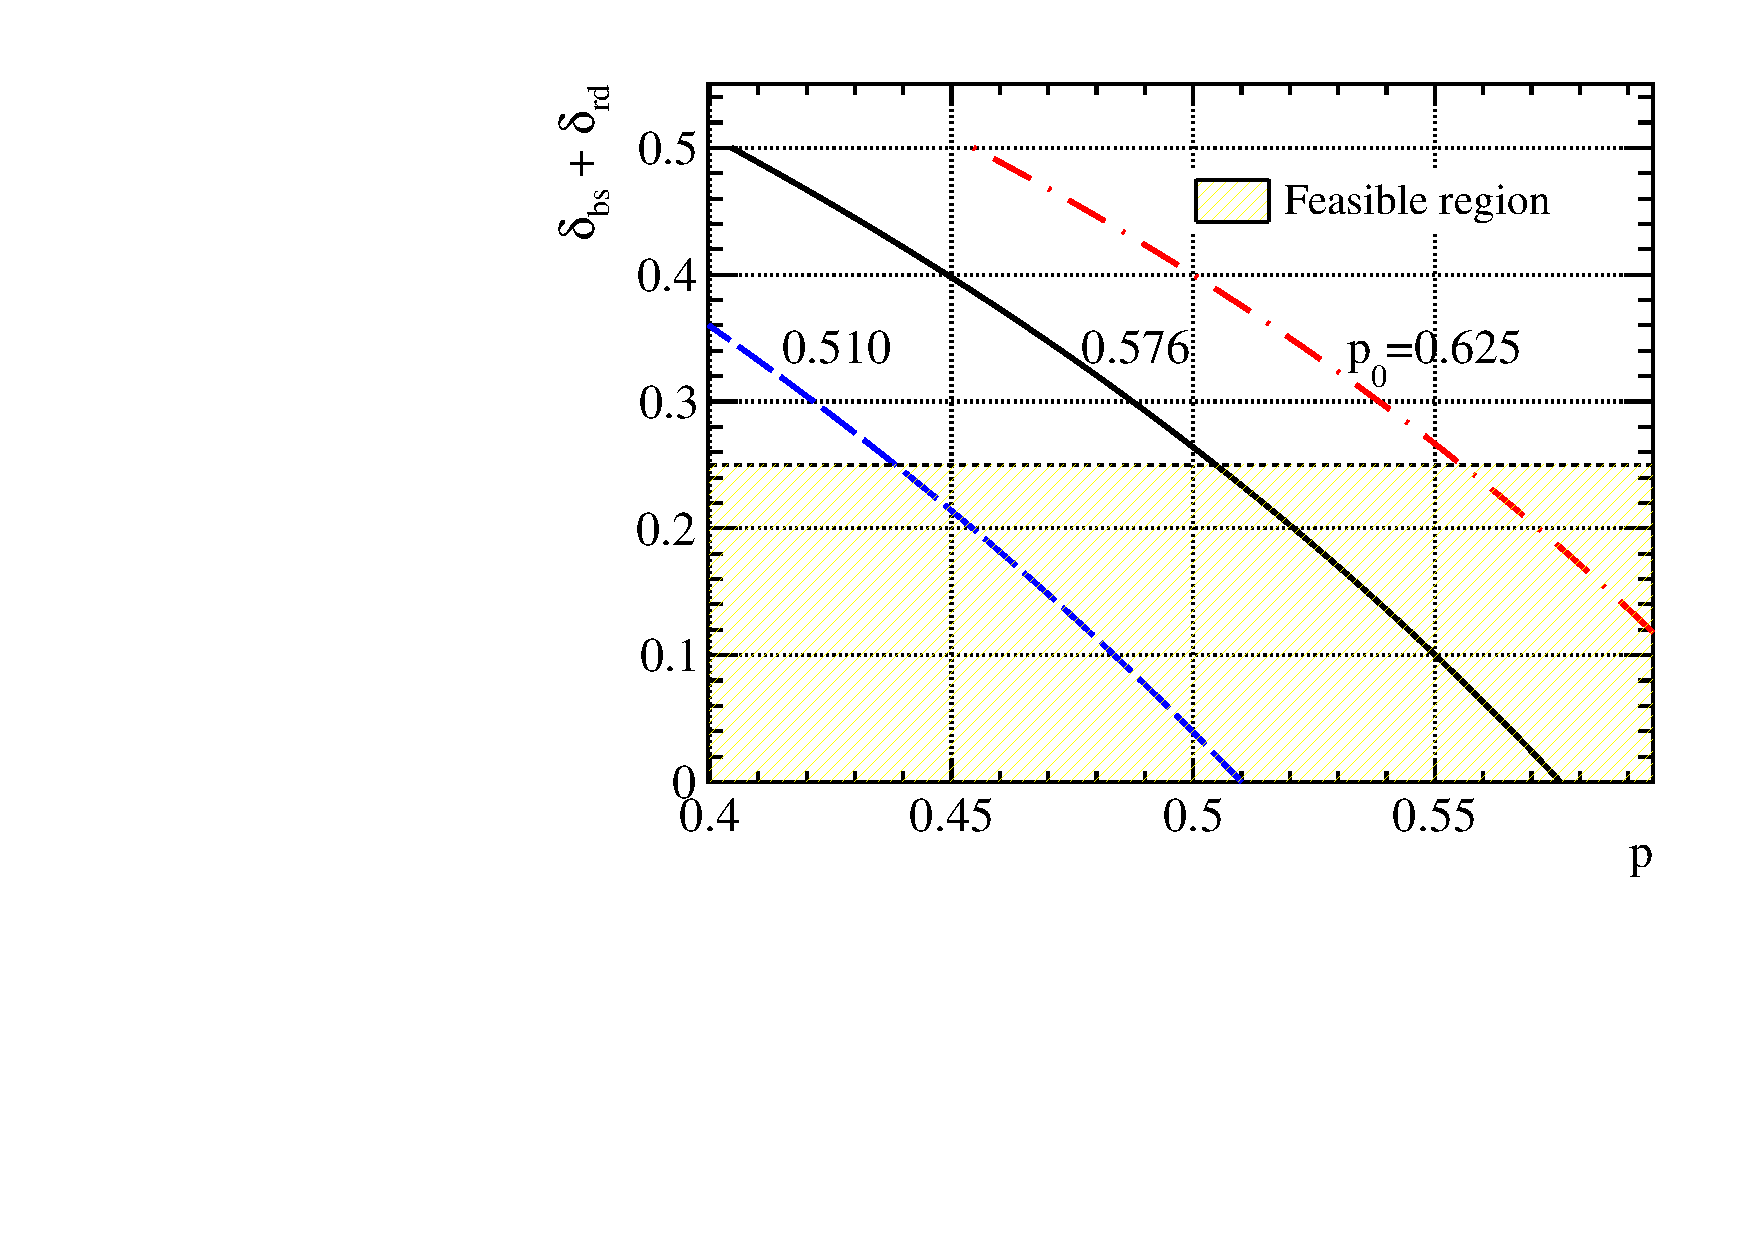
\includegraphics[width=\linewidth]{PMTRelated/GTmodel/parameter_pp0.pdf}
		\caption{}
		\label{fig:pp0}
	\end{subfigure}
	\hfill
	\begin{subfigure}{0.48\textwidth}
		\centering
		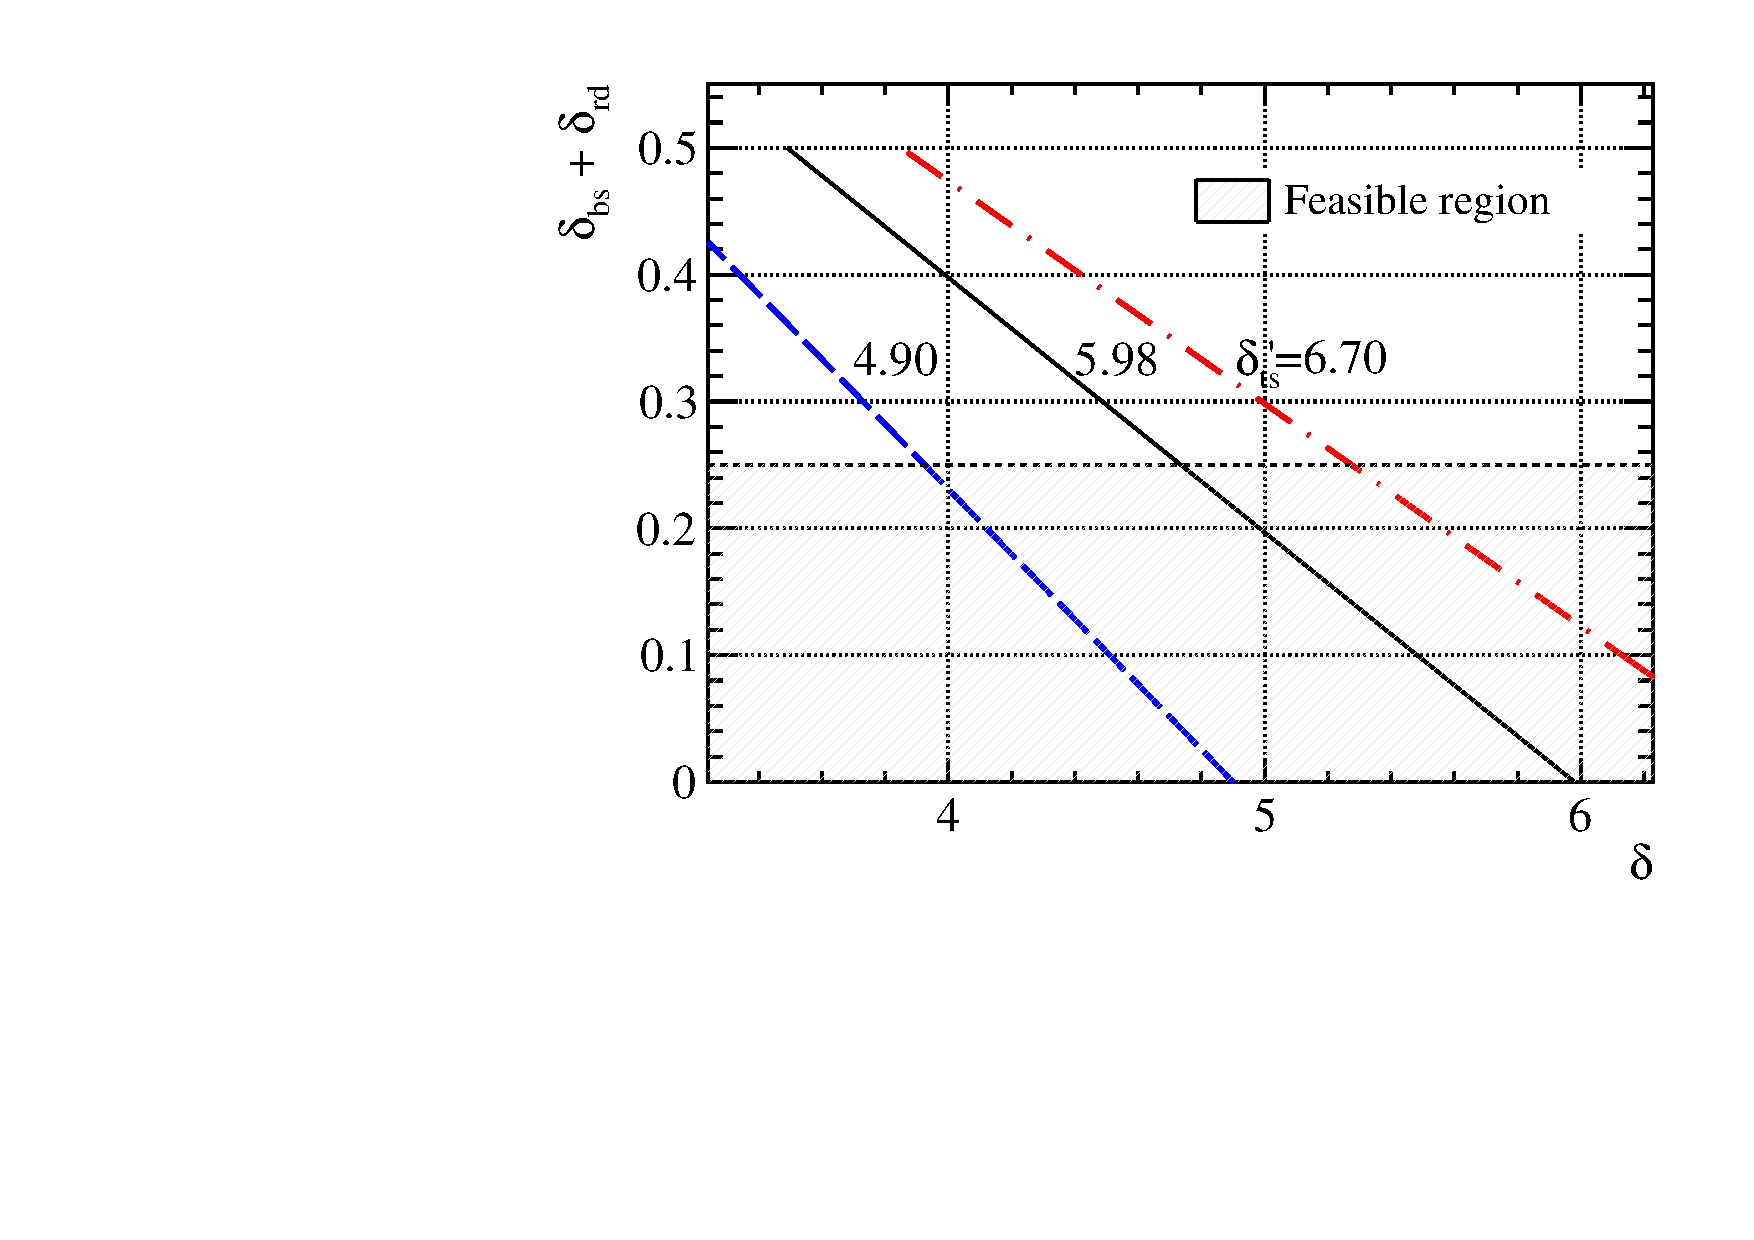
\includegraphics[width=\linewidth]{PMTRelated/GTmodel/parameters_ts.pdf}
		\caption{}
		\label{fig:tsts}
	\end{subfigure}
	\caption{Relations of \(\delta_\text{bs} + \delta_\text{rd}\) against the SEY \(\delta\) and the fraction of channel mode \(p\).
		The feasible region shows the consistency of our measurement to the literature.}
	\label{fig:pdelta}
\end{figure}

In Fig.~\ref{fig:pdelta}, with the typical values of \(\delta=5\) and \(p=0.55\),
our measurement is consistent with an assumption that \(\delta_\text{bs} + \delta_\text{rd} < 0.25\).
The small contribution of the back-scattered and rediffused electrons in SEE is pointed out by Beck~\cite{beck_physical_1966} to be especially true for insulators with high SEY.


\subsection{Gamma-Tweedie model for MCP-PMT}\label{sec:model}
In our calculation, the distribution of the MCP charge response to the true-secondary electrons $\varGamma(\alpha_{i},\beta_{i})$ is determined by their energies $E_{i}$,
which satisfy $\sum_{i}^{n}E_{i}<E_0$.
The incident energy \(E_0\) of the PEs is \SI{650}{eV},
which is more than ten times the energies of the true secondaries.
Because $n$ follows a Poisson distribution with an expectation between 5 and 6.5,
the probability of $n$ exceeding 10 is negligible.
Thus, the effect of $n$ on $E_{i}$ can be ignored,
and the energy \(E_{i}\) is independently and identically distributed, as demonstrated in Fig.~\ref{fig:single_pe}.
The charge response of MCP to a single true-secondary electron, in turn, can be treated identically, as shown in Fig.~\ref{fig:single_fit}.
Furthermore, a single Gamma distribution \(\varGamma(\alpha',\beta')\)
is flexible enough to describe the continuous mixture of
\(\int dE_{i}\frac{1}{\delta_{\mathrm{ts}}}\frac{d\delta_{\mathrm{ts}}}{dE_{i}}\varGamma[\alpha(E_{i}),\beta(E_{i})]\).

\begin{figure}[!htbp]
	\centering
	\begin{subfigure}{0.47\textwidth}
		\centering
		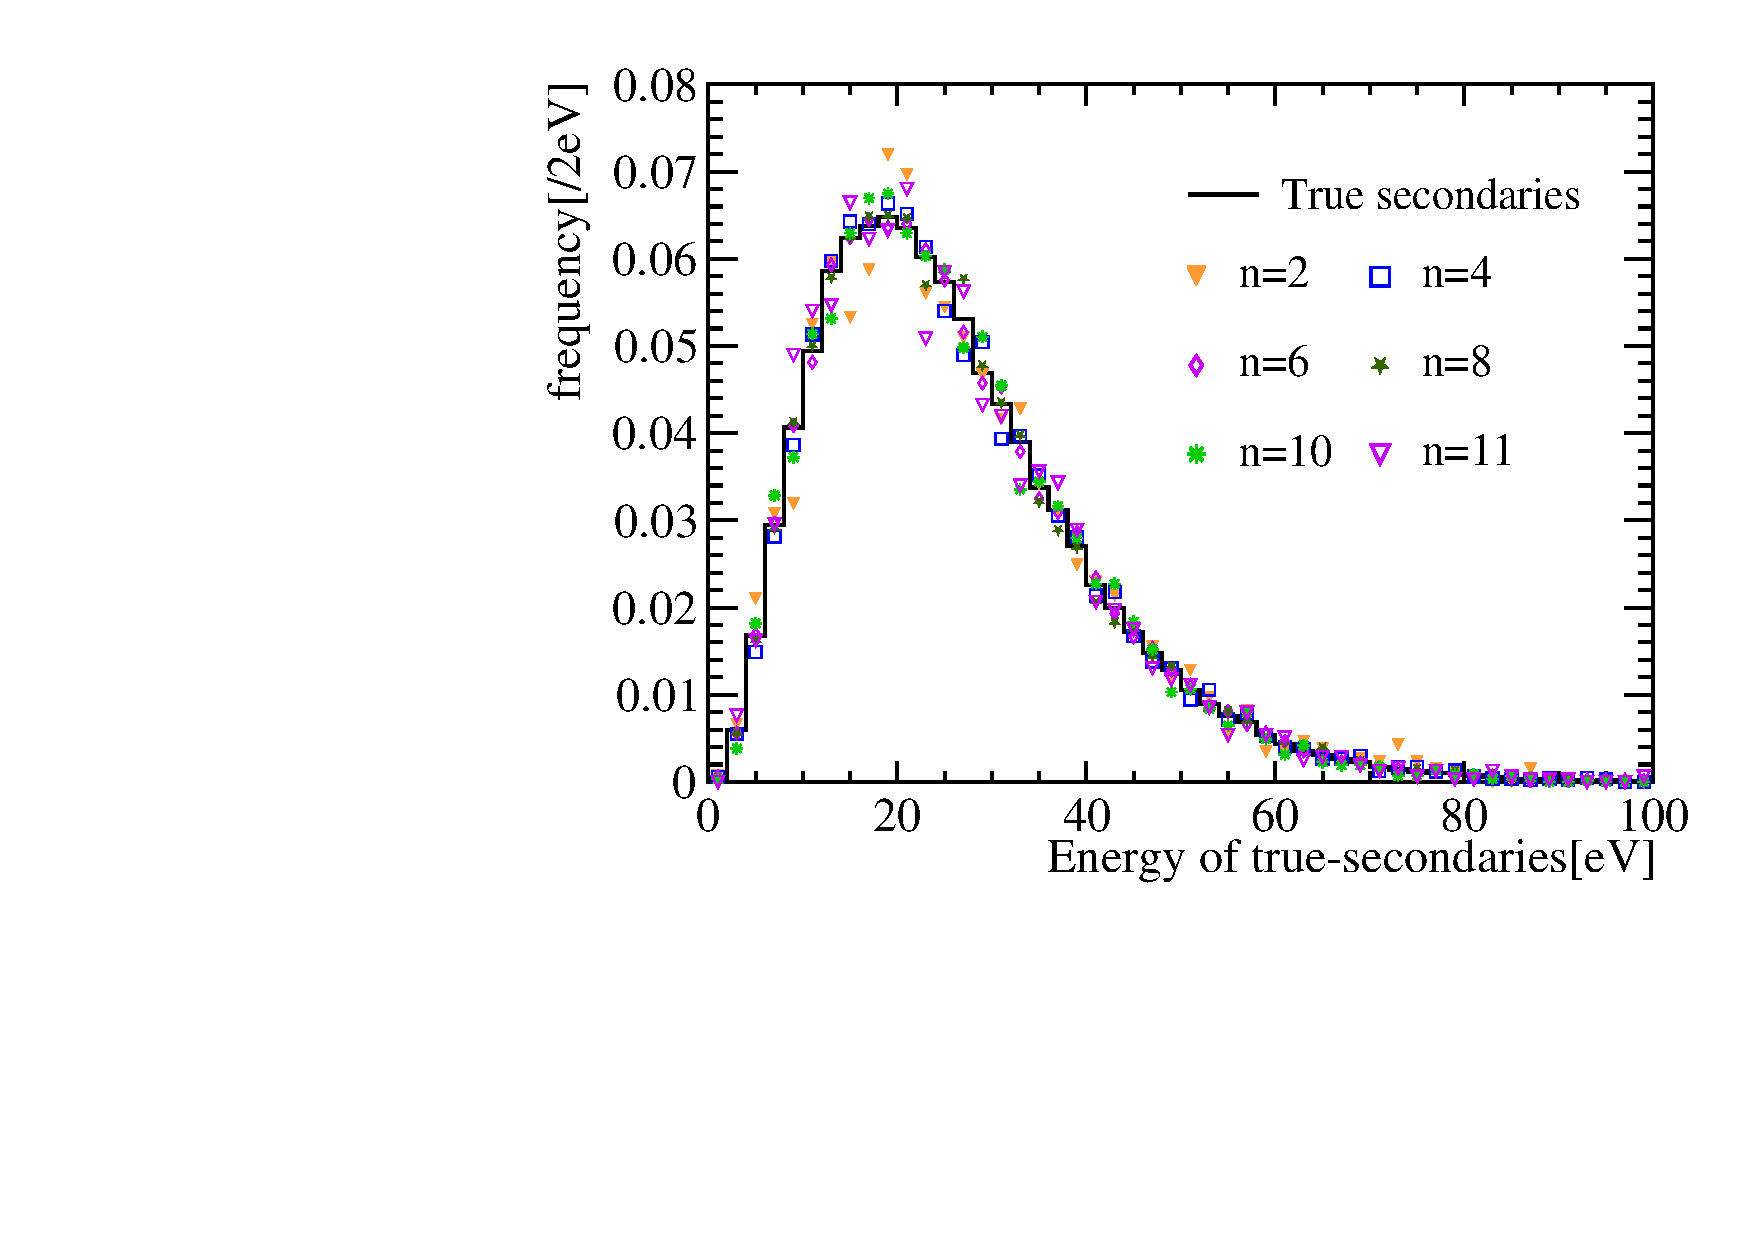
\includegraphics[width=\linewidth]{PMTRelated/GTmodel/single_pecharge.pdf}
		\caption{}
		\label{fig:single_pe}
	\end{subfigure}
	\hfill
	\begin{subfigure}{0.47\textwidth}
		\centering
		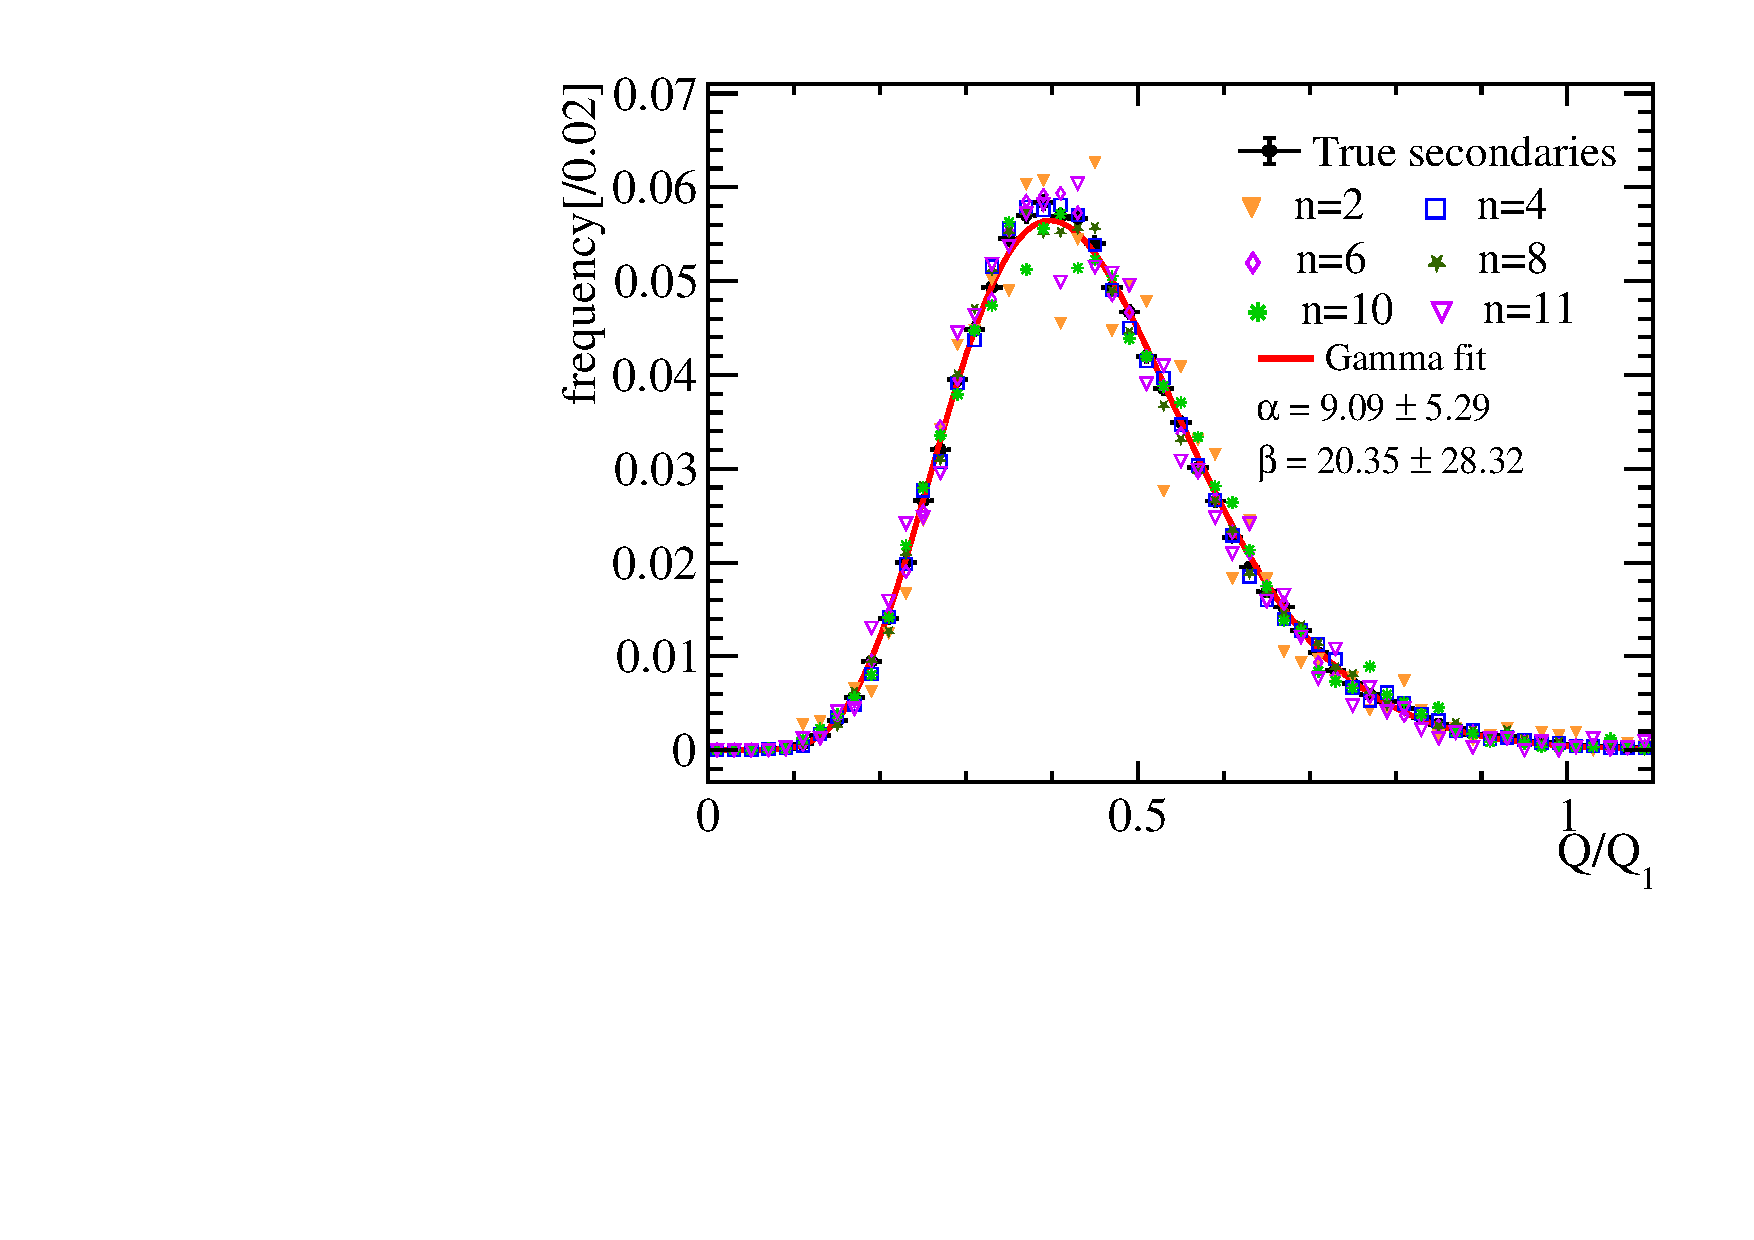
\includegraphics[width=\linewidth]{PMTRelated/GTmodel/singlepefit.pdf}
		\caption{}
		\label{fig:single_fit}
	\end{subfigure}
	\caption{The energy distribution and the charge response distribution of MCP to a single true-secondary electron when $n$ is different.
		\subref{fig:single_pe}: All the energies of the true secondaries follow the same distribution,
		although $n$ is different.
		\subref{fig:single_fit}: the charge response of MCP to a single true-secondary electron is identical,
		and the fitting of the Gamma distribution~\(\varGamma(\alpha',\beta')\)
		achieves sufficient goodness.}
	\label{fig:singlepe}
\end{figure}

When we use such a single \(\varGamma(\alpha', \beta')\) in Eq.\eqref{eq:ts_all},
the resulting Poisson-Gamma compound is a special case of the Tweedie distribution $\mathrm{Tw}_{\xi}(\alpha,\beta)$
for $1<\xi<2$~\cite{1991Tweedie}.
\begin{equation}
	\arraycolsep=1.4pt
	\label{eq:ts_gamma}
	\left.\begin{array}{rl}
		Q_{\text{ts}} & = \sum_{{i}=1}^{n} Q_{i}                 \\
		n             & \sim \mathrm{\pi}(\delta_{\mathrm{ts}}') \\
		Q_{i}         & \sim \varGamma(\alpha', \beta')
	\end{array}\right\} \implies
	Q_{\text{ts}} \sim \mathrm{Tw}_{\xi}(\alpha',\beta')
\end{equation}
A phenomenological joint fit of the \(f_\mathrm{ch}\) Gamma and \(f_\mathrm{ts}\) Tweedie
mixture with Eq.~\eqref{eq:1} and \eqref{eq:ts_gamma} is sufficient to calibrate the SER charge spectrum and measure \(p_0\) and \(\delta_\text{ts}'\).
The voltage division experiment~(Sec.~\ref{sec:gain}) relations \(\mu(E_i)\)/\(\sigma(E_i)\) and the Furman model provide the understanding of the jumbo charges and the justification of the phenomenological Gamma-Tweedie
mixture, but are less practically useful in PMT calibrations.

The number of parameters, 2 for \(f_\mathrm{ch}\) Gamma and 3 for \(f_\mathrm{ts}\) Tweedie,
hinders convergence unless we aid it with physical constraints.
Typically $\frac{\alpha'}{\beta'}\approx 0.45Q_1$ and \(\sqrt{\frac{\alpha'}{\beta'^2}}\approx 0.15Q_1\).
It is practical to bound them in $[0.3,0.7]Q_1$ and $[0.05,0.3]~Q_1$ when the incident energy $E_0$ is significantly greater than $E_{i}$.
We also have checked the chi-square results in the Gamma-Tweedie fitting,
which gives good $\chi^2/\mathrm{ndf}<10$.

In this case, we can write the mathematical model for the SER of the MCP-PMT:
\begin{equation}
	\label{eq:GTmodel}
	f_{\text{MCP-PMT}}(Q) = p_0 \varGamma(Q; \alpha, \beta) + (1-p_0) \mathrm{Tw}_{\xi}(Q; \alpha', \beta')
\end{equation}
We can get the peak gain $G_p=\alpha/\beta$ and average gain $G_m=p_0\alpha/\beta+(1-p_0)\delta_{\mathrm{ts}}'\alpha'/\beta'$.

\section{The timing calibration}

\section{The dark count rate}

\chapter{The reconstruction for the water-phase}
\label{chap:recon}
After carefully calibrating the PMTs, we can obtain the number of photons hitting the PMT and their arrival times for each event. Based on these information, we will use statistical methods to infer information such as the position, energy, and direction of the physical events that produced these photons.
In the field of Cherenkov reconstruction, the Super-Kamiokande~(SK) experiment is the most worthy of reference. SK stands as the world's largest pure water Cherenkov detector, housing \SI{50}{kilotons} of ultrapure water~\cite{SK}. Building upon the liquid scintillator-Cherenkov combined track reconstruction technique developed for the MiniBooNE experiment~\cite{minibone}, SK collaboration has advanced a likelihood-based reconstruction method, utilizing PMT charge and time information~\cite{SKfiTQun}, named as fiTQun. For JUNO water-phase, we have implemented targeted improvements to the fiTQun and extended its application to low-energy event reconstruction at the \si{MeV} scale.

\section{The Likelihood function}
\label{sec:recon}
FiTQun simultaneously determines particle types, vertex positions, momentums, event times.
In JUNO water-phase, we just need to determine the vertex position, momentums and event times.
The likelihood function of fiTQun is defined as:
\begin{equation}
	\begin{aligned}
		\log \mathcal{L}(\boldsymbol{x};{q},{t}) = & \sum_{j \in \{q=0\}} \log P_j \bigl( q=0\bigm| \mu_j \bigr)                                      \\
		                                           & + \sum_{i \in \{q>0\}} \log \bigl( f_{\mathrm{q}}\bigl( q_i \bigm| \mu_i \bigr) \bigr)           \\
		                                           & + \sum_{i \in \{q>0\}} \log \bigl( f_{\mathrm{t}} \bigl( t_i \bigm| \boldsymbol{x} \bigr) \bigr)
	\end{aligned}
\end{equation}
\begin{itemize}
	\item $\boldsymbol{x} = (t_0, x, y, z, p_x, p_y, p_z)$: Event vertex containing time $t_0$, position $(x,y,z)$, and momentum $(p_x,p_y,p_z)$.
	\item $\mu_i(\boldsymbol{x})$: Expected PEs at the $i$-th PMT, computed from the vertex $\boldsymbol{x}$.
	\item $q_i$: Charge observed at the $i$-th PMT, $\{q\}$ is the sequence of $q_i$, when $q_i=0$, the PMT is unhitted.
	\item $t_i$: Hit time of the $i$-th PMT, $\{t\}$ is the sequence of $t_i$.
\end{itemize}

The first term is the unhit likelihood, which is the probability of no hit in the PMT. The second term is the hit likelihood, which is the probability of detecting hits in the PMT. The third term is the time likelihood, which is the probability of detecting a hit at a certain time.

Since in the operation of the detector, only TQ information (time and charge) is recorded for low-energy events, waveform information is unavailable. At the same time only the first hit time can be obtained. Therefore, it is necessary to reformulate the likelihood to adopt a first-hit-time-based reconstruction approach. Xuewei Liu~et.al developed a first-principles-based reconstruction method using time-charge information or time-PE information in liquid scintillator detectors~\cite{Liu:2024cxo}. We adapt their methodology to reformulate the likelihood function for JUNO water-phase. In low-energy events, where each PMT typically detects only few photon, the number of hits can be directly approximated as NPE~($N_{PE}$). We can reformulate the likelihood function as Eq.~\eqref{eq:likelihood}:
\begin{equation}
	\begin{aligned}
		\log \mathcal{L}(\boldsymbol{x};{q},{t})= & \sum_{j \in \{q=0\}}\log P_j \bigl( q=0\bigm| \mu_j \bigr)+                                                                                                                  \\
		                                          & \sum_{i \in \{q>0\}} \log \bigl( f_{\mathrm{q}}\bigl( 0 \bigm| \mu_{i,T_{low}}^{T_i} \bigr) * f_{\mathrm{t}}(T_i) * f_{\mathrm{q}}(N_{PE,i}-1|\mu_{i,T_{i}}^{T_{up}}) \bigr)
	\end{aligned}
	\label{eq:likelihood}
\end{equation}

In this case, we define the data taking as $[T_{low},T_{up}]$, and the first hit time of the $i$-th PMT as $T_{i}$, $\mu_{i,T_{low}}^{T_i}$ is the expected PEs in [$T_{low}$,${T_i}$], same as $\mu_{i,T_{i}}^{T_{up}}$.

\section{Response of the water-phase dector}
To compute the likelihood, we need to predict how many photons each PMT will detect when given a vertex. The more accurate the predictions are, the better the reconstruction performances. Therefore, we need a comprehensive understanding of the detector response and develop accurate models for it.
It naturally comes to mind that when a charged particle enters water, emits Cherenkov photons, and triggers the PMT, this process can be divided into two parts. One pertains to how Cherenkov light is emitted, while the other concerns how the Cherenkov photons propagate and are detected.

\subsection{The Cherenkov emission profile}
When a charged particle travels through a medium at a speed exceeding that of light, it emits Cherenkov photons within a specific solid angle range. The phenomenon arises from local polarization occurring along the charged particle's trajectory: when polarized molecules return to their ground state, they emit electromagnetic radiation. When the refractive index of the medium is $n$, and the speed of light in vacuum is $c_0$, the condition of particle speed~$v_p$ for Cherenkov emmision is $\beta=v_p/c_0>1/n$. When in pure water, whose refractive index is $n_w=1.333$, and the paitical is electron~($m_0=\SI{0.511}{MeV}$), the energy threthold is $E_{th}=m_0\times(\sqrt{1-1/n_w^2}-1)=\SI{0.262}{MeV}$. That means, only when the energy of electron is larger than \SI{0.262}{MeV}, the Cherenkov photons will emit.

The direction of Cherenkov photons can be discribed as: $\cos\theta=\frac{1}{\beta n_w}$ as Fig~\ref{Fig:Cherenkov_emmision} shown.

\begin{figure}
	\begin{center}
		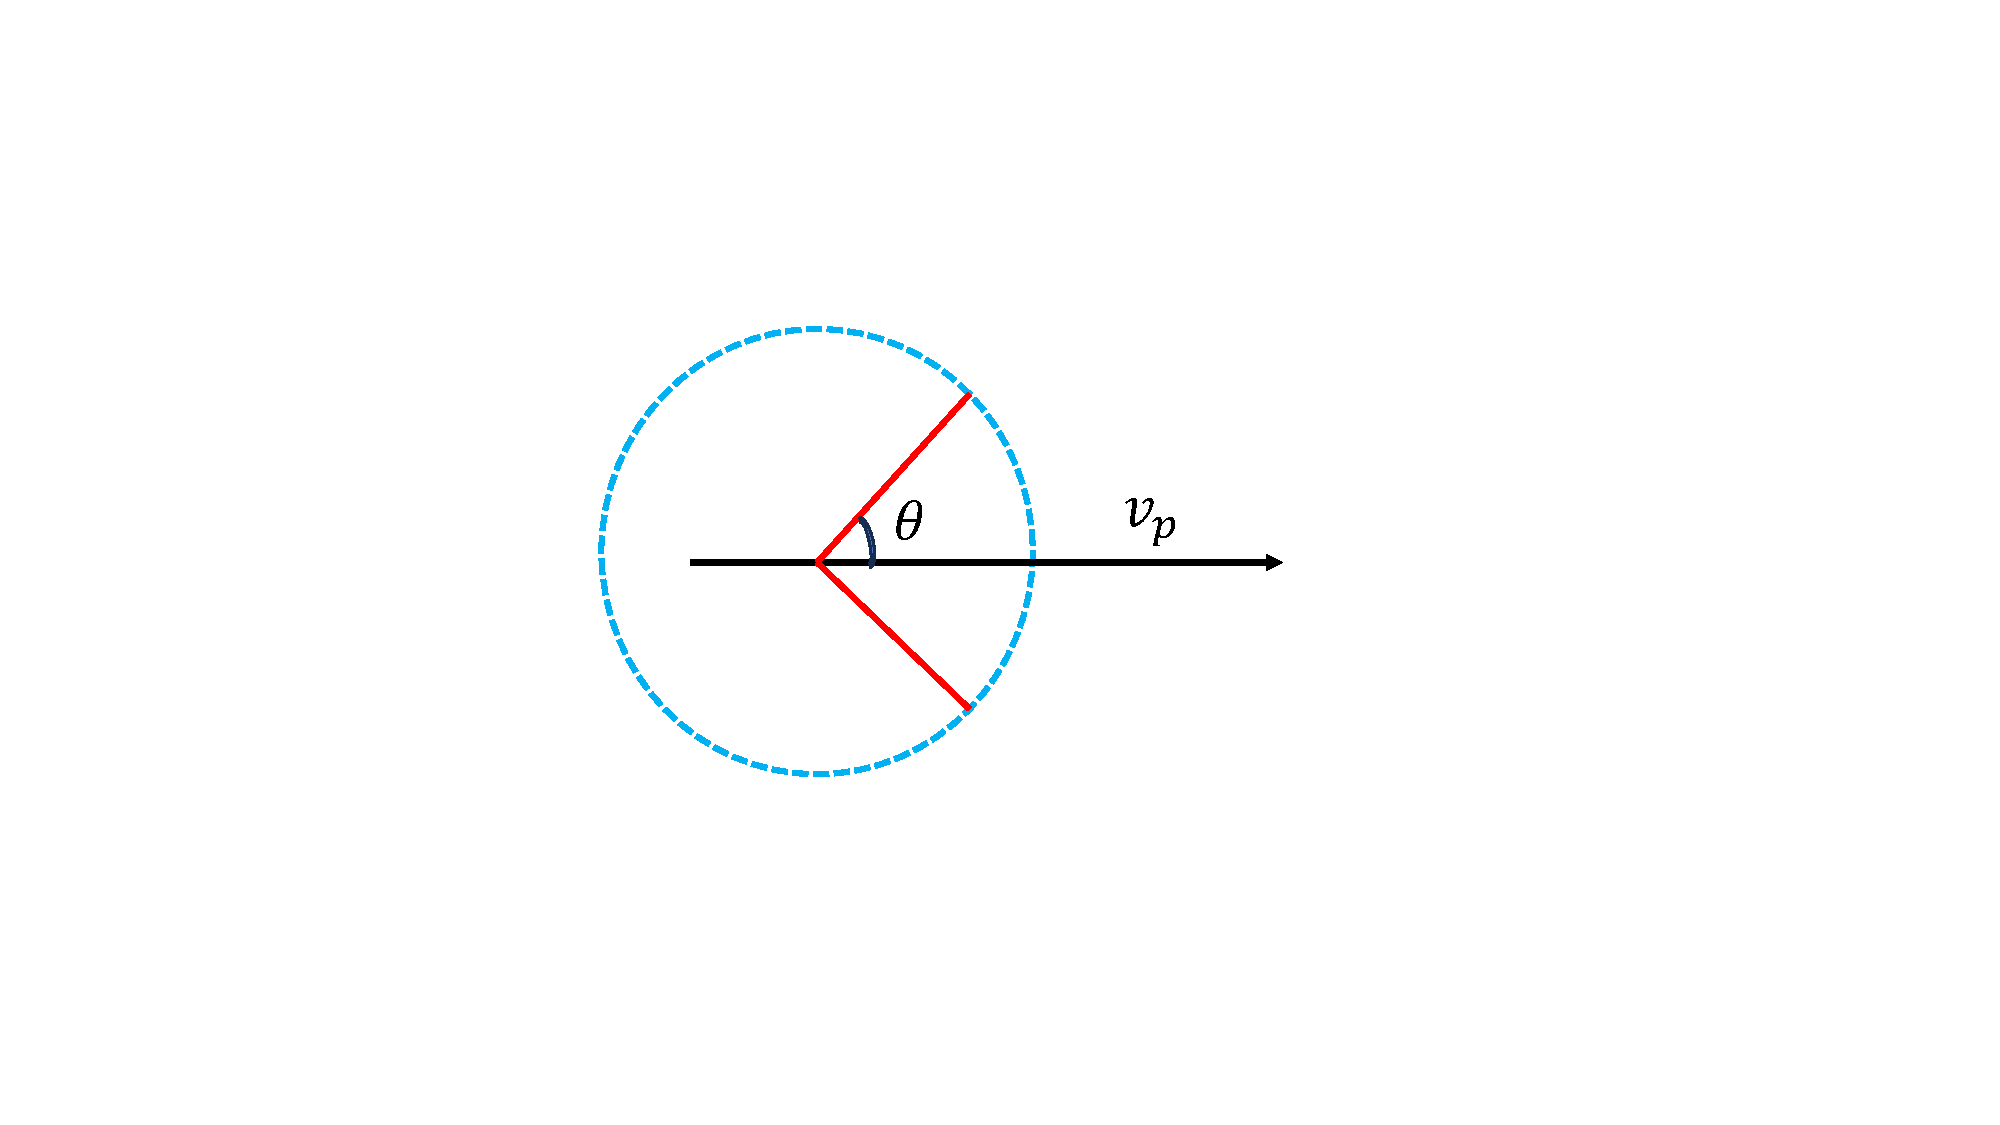
\includegraphics[height=6cm]{reconstruction/cherenkov_emission.pdf}
	\end{center}
	\caption{The direction of Cherenkov photons. $\theta$ is the angle between the photon emission direction and the direction of particle motion.}
	\label{Fig:Cherenkov_emmision}
\end{figure}

When in water, $\cos\theta\approxeq0.75$. We can use simulation to get the emmision profile of Cherenkov photons. Also, we consider the light yield of Cherenkov by simulating electron with momentum from \SI{2}{MeV} to \SI{30}{MeV}. Our simulation is based on JUNO software~(JUNOsw)~\cite{junosw}, and the version is J24.2.1. We simulated electrons with momenta ranging from 2 to \SI{50}{MeV}, uniformly distributed within the detector, while their emission directions were randomly oriented.

We extended Dou Wei's angular coordinate definition method for liquid scintillator detectors~\cite{Dou:2022} to Cherenkov radiation detection by incorporating momentum direction degrees of freedom, resulting in the coordinate system illustrated in the figure.

\begin{figure}
	\begin{center}
		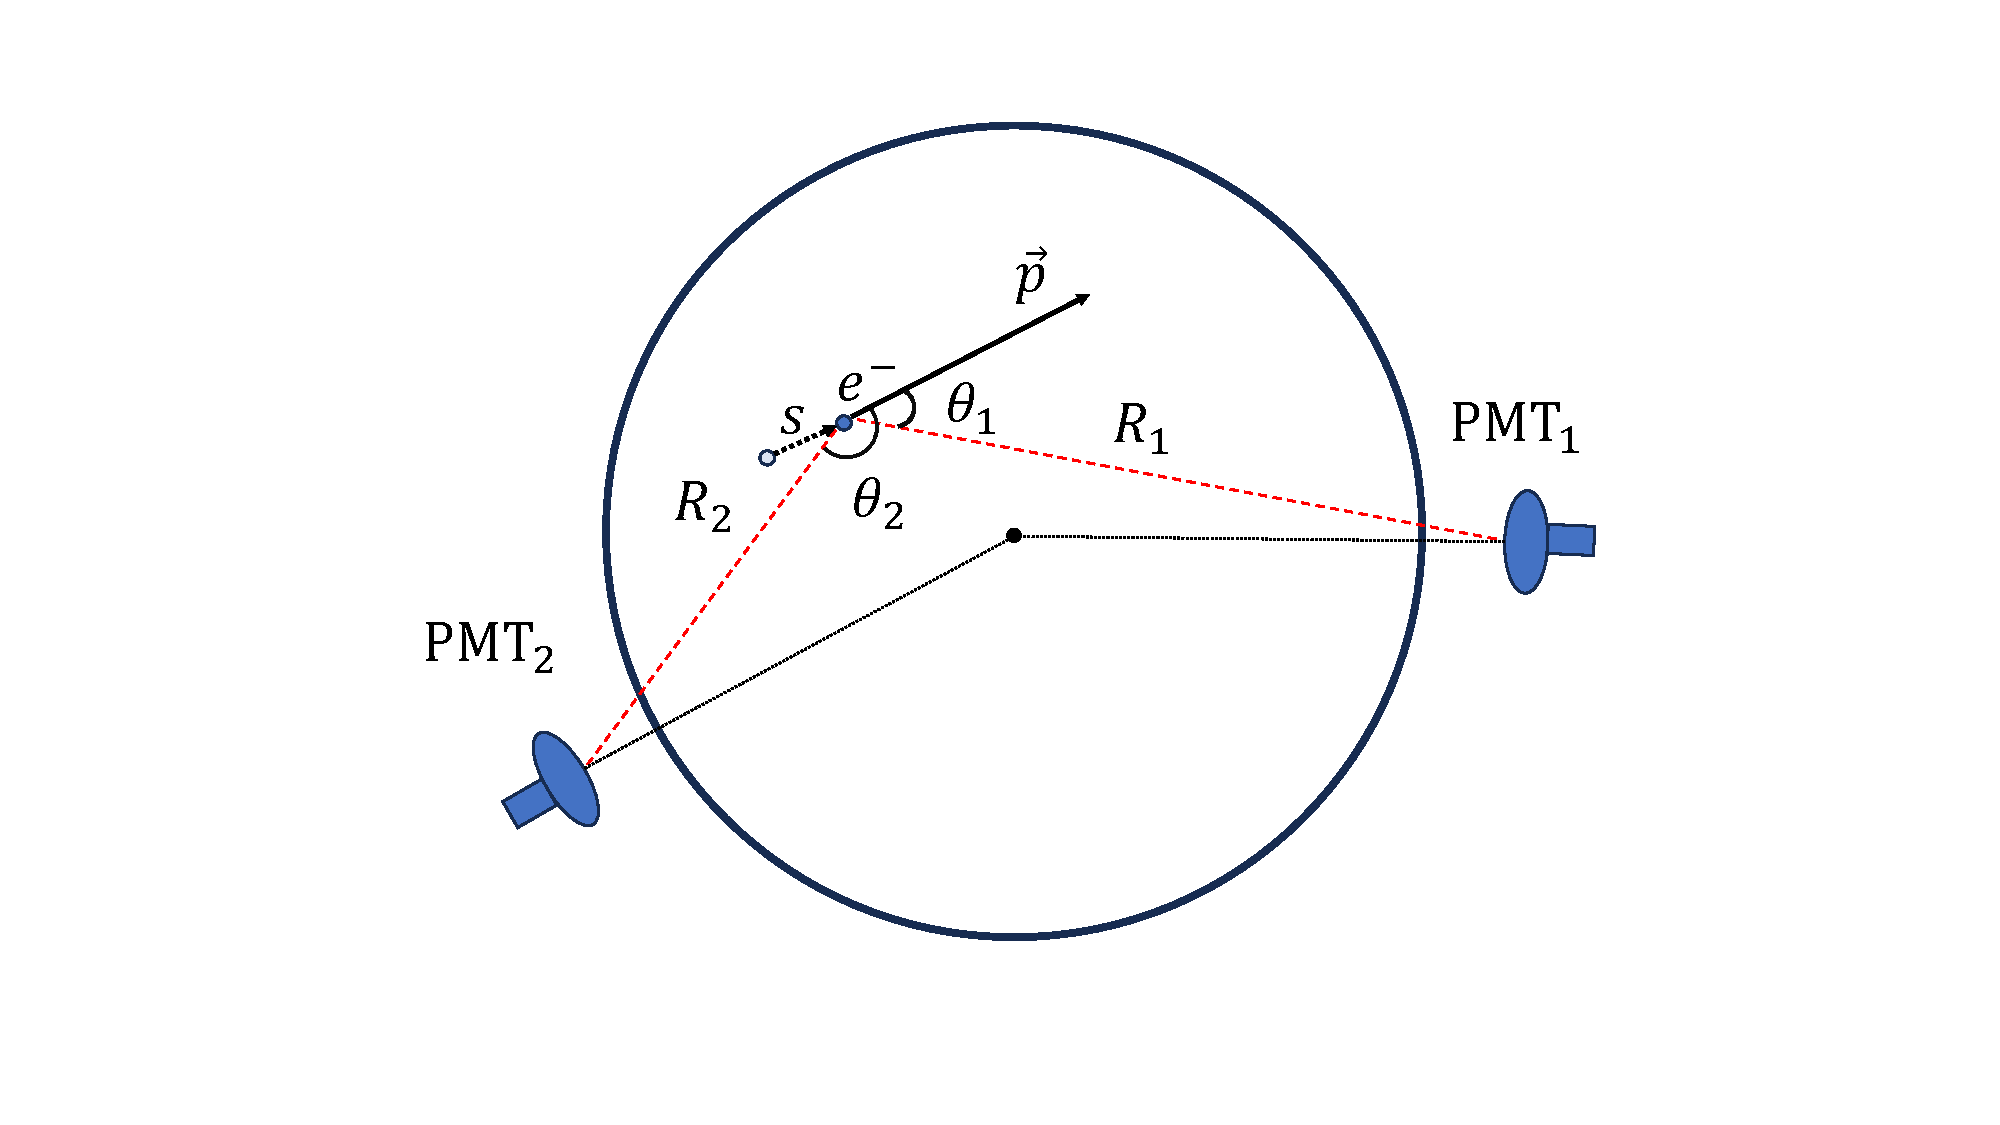
\includegraphics[height=6cm]{reconstruction/zuobiao.pdf}
	\end{center}
	\caption{Coordinate system definition: $\theta$ is the angle of the emission direction of Cherenkov photon and the incident direction of the electron, $s$ is the distance from the position where the particle emits light to its initial position. $R$ is the distance of PMT to the position of electron.}
	\label{Fig:Coordinate}
\end{figure}

In this simulation, we recorded the angles between the emission directions of all Cherenkov photons and the incident direction of the electron, and we do not care the photons are detected or not. Simultaneously, a crucial parameter is the distance between the photon generation point and the origin position of the charged particle.
\begin{itemize}
	\item From Fig~\ref{fig:thetaemmision}, most photons are emitted along the Cherenkov angle~($\cos\theta=0.75$), while a minority exhibit significant angular deviations from the electron's direction. When calculating the emission angle distribution, it must be analyzed separately for different particle energies rather than applying a single angular distribution to electrons of all energies.
	\item From Fig~\ref{fig:semmision}, as the particle moves, Cherenkov photons emitted along the initial segment of its trajectory exhibit a uniform distribution. When the particle's velocity significantly decreases, photon emission drops markedly, with the vast majority of photons being emitted within the first half of the trajectory.
	\item From Fig~\ref{fig:tsemmision}, after traveling some distance, the probability of photons deviating from the Cherenkov angle gradually increases due to multiple scattering. As illustrated in the figure, when electrons undergo multiple scattering, their direction changes significantly, as Fig~\ref{fig:multipleScattering} shown. However, when calculating the Cherenkov emission angle, we still use the initial incident direction, thereby producing photons emitted at angles far from the ideal Cherenkov angle.
	\item In this case, we get the Cherenkov emmision profile~($g(p,s,\theta)$) which describes the proportion of Cherenkov photons emitted at specific locations and directions along the trajectory of a charged particle with a given energy, relative to the total number of emitted photons. For the convenience of research, we use momentum~($p$) instead of energy~($E$).
\end{itemize}

\begin{figure}[htbp]
	\centering
	\begin{subfigure}{0.475\textwidth}
		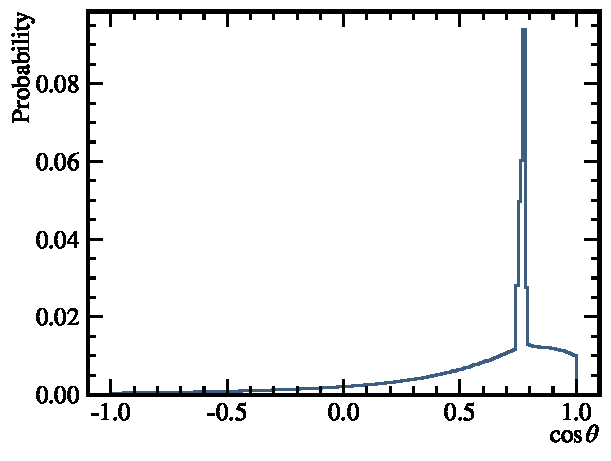
\includegraphics[page=1,width=\textwidth]{reconstruction/emmisionProfile/2.pdf}
		\caption{\SI{2}{MeV} electron}
		\label{fig:theta2mev}
	\end{subfigure}
	\hfill
	\begin{subfigure}{0.475\textwidth}
		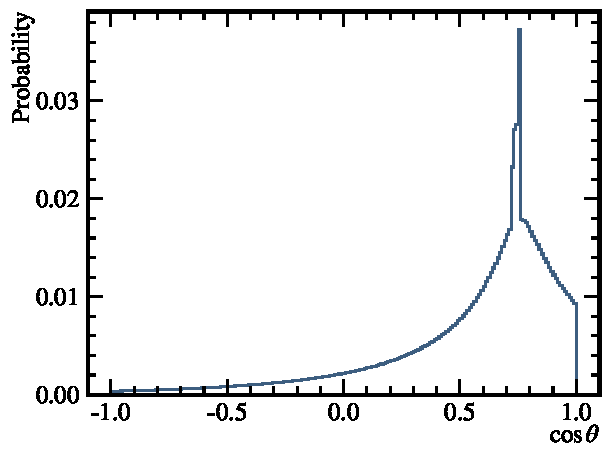
\includegraphics[page=1,width=\textwidth]{reconstruction/emmisionProfile/5.pdf}
		\caption{\SI{5}{MeV} electron}
		\label{fig:theta5mev}
	\end{subfigure}

	\vspace{\baselineskip}

	\begin{subfigure}{0.475\textwidth}
		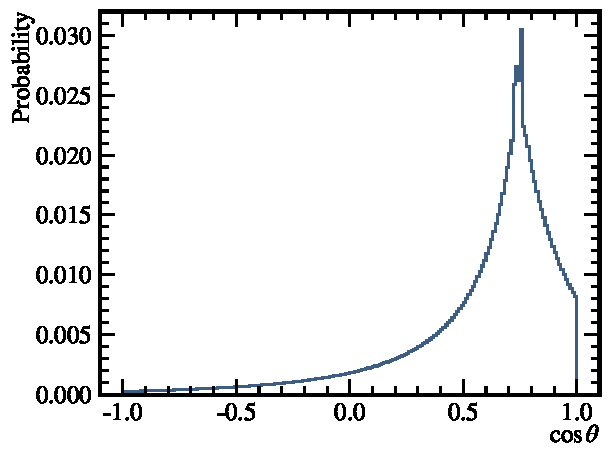
\includegraphics[page=1,width=\textwidth]{reconstruction/emmisionProfile/10.pdf}
		\caption{\SI{10}{MeV} electron}
		\label{fig:theta10mev}
	\end{subfigure}
	\hfill
	\begin{subfigure}{0.475\textwidth}
		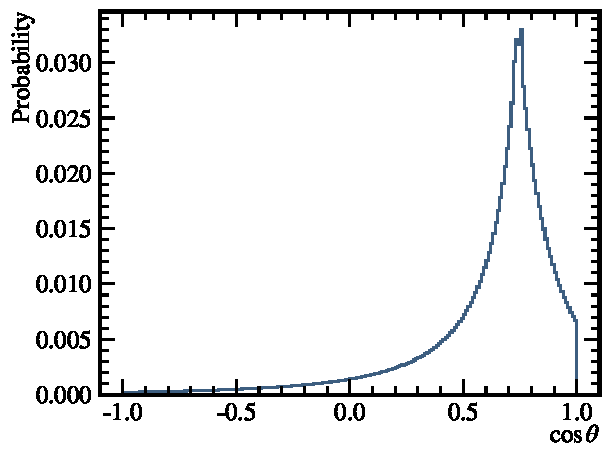
\includegraphics[page=1,width=\textwidth]{reconstruction/emmisionProfile/20.pdf}
		\caption{\SI{20}{MeV} electron}
		\label{fig:theta20mev}
	\end{subfigure}
	\caption{The relationship of emission probability with $\cos\theta$.}
	\label{fig:thetaemmision}
\end{figure}

\begin{figure}[htbp]
	\centering
	\begin{subfigure}{0.475\textwidth}
		\includegraphics[page=2,width=\textwidth]{reconstruction/emmisionProfile/2.pdf}
		\caption{\SI{2}{MeV} electron}
		\label{fig:s2mev}
	\end{subfigure}
	\hfill
	\begin{subfigure}{0.475\textwidth}
		\includegraphics[page=2,width=\textwidth]{reconstruction/emmisionProfile/5.pdf}
		\caption{\SI{5}{MeV} electron}
		\label{fig:s5mev}
	\end{subfigure}

	\vspace{\baselineskip}

	\begin{subfigure}{0.475\textwidth}
		\includegraphics[page=2,width=\textwidth]{reconstruction/emmisionProfile/10.pdf}
		\caption{\SI{10}{MeV} electron}
		\label{fig:s10mev}
	\end{subfigure}
	\hfill
	\begin{subfigure}{0.475\textwidth}
		\includegraphics[page=2,width=\textwidth]{reconstruction/emmisionProfile/20.pdf}
		\caption{\SI{20}{MeV} electron}
		\label{fig:s20mev}
	\end{subfigure}
	\caption{The relationship of emission probability with $s$.}
	\label{fig:semmision}
\end{figure}


\begin{figure}[htbp]
	\centering
	\begin{subfigure}{0.475\textwidth}
		\includegraphics[page=3,width=\textwidth]{reconstruction/emmisionProfile/2.pdf}
		\caption{\SI{2}{MeV} electron}
		\label{fig:ts2mev}
	\end{subfigure}
	\hfill
	\begin{subfigure}{0.475\textwidth}
		\includegraphics[page=3,width=\textwidth]{reconstruction/emmisionProfile/5.pdf}
		\caption{\SI{5}{MeV} electron}
		\label{fig:ts5mev}
	\end{subfigure}

	\vspace{\baselineskip}

	\begin{subfigure}{0.475\textwidth}
		\includegraphics[page=3,width=\textwidth]{reconstruction/emmisionProfile/10.pdf}
		\caption{\SI{10}{MeV} electron}
		\label{fig:ts10mev}
	\end{subfigure}
	\hfill
	\begin{subfigure}{0.475\textwidth}
		\includegraphics[page=3,width=\textwidth]{reconstruction/emmisionProfile/20.pdf}
		\caption{\SI{20}{MeV} electron}
		\label{fig:ts20mev}
	\end{subfigure}
	\caption{The relationship of emission probability with $s$ and $\cos\theta$.}
	\label{fig:tsemmision}
\end{figure}

\begin{figure}
	\begin{center}
		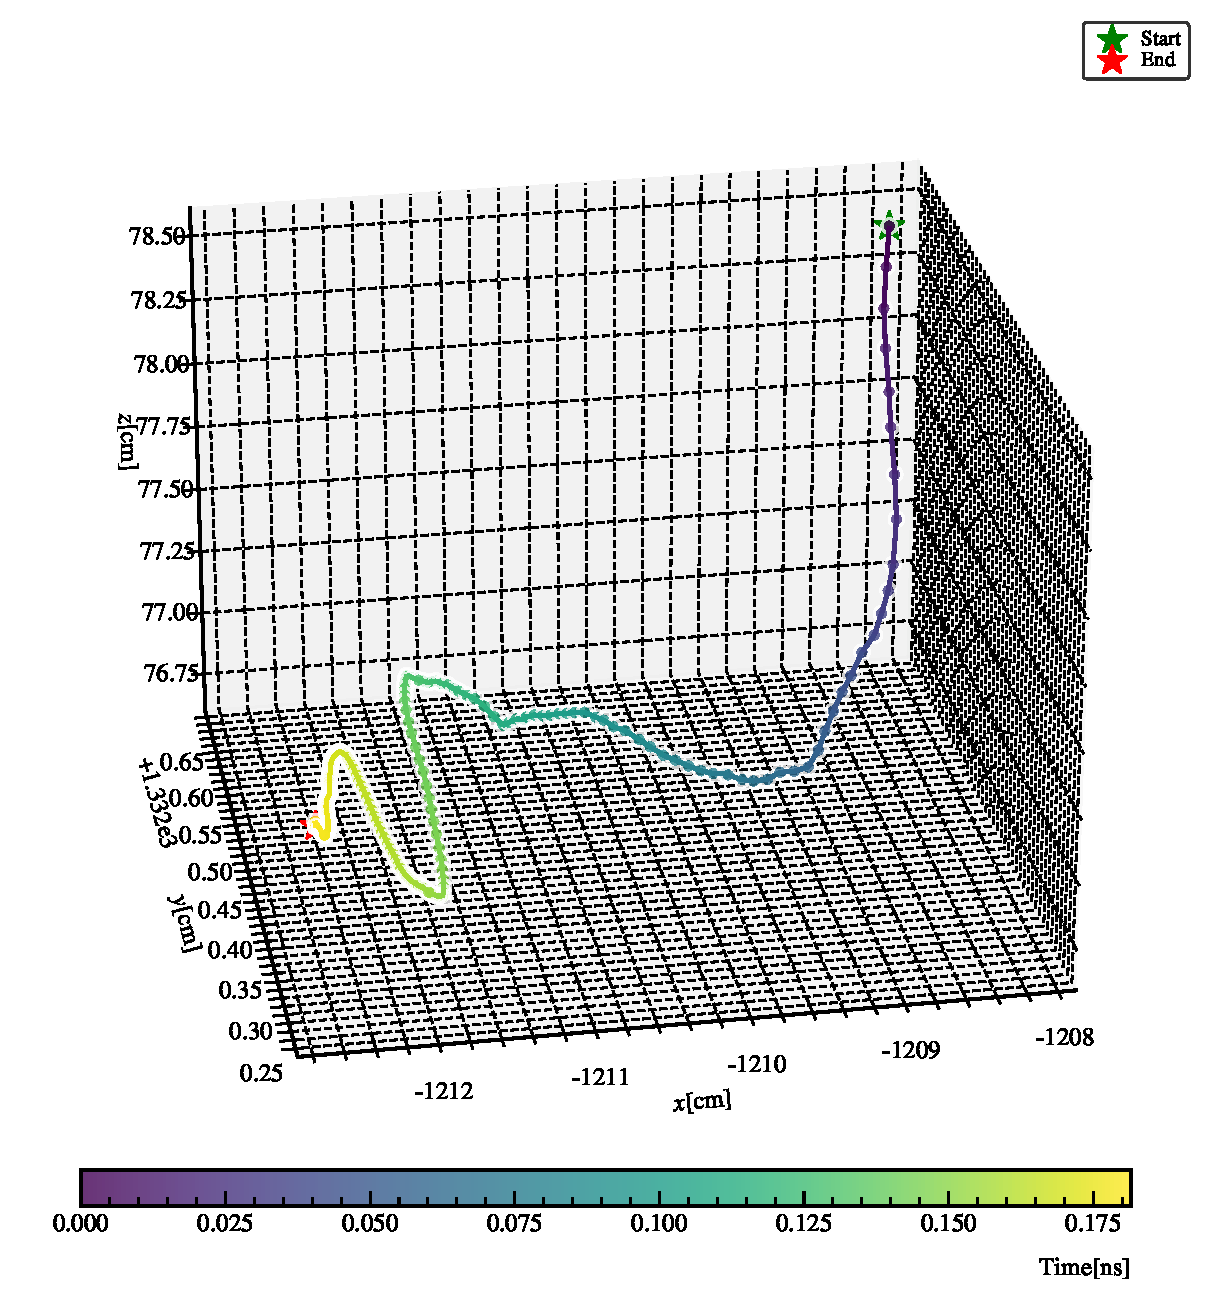
\includegraphics[width=\textwidth]{reconstruction/emmisionProfile/multiscatter.pdf}
	\end{center}
	\caption{An example of a \SI{10}{MeV} electron undergoing multiple scattering.}
	\label{fig:multipleScattering}
\end{figure}

Through Gaussian fitting as shown in Fig~\ref{fig:yield_gauss_fit} in simulation, we obtain the total number of photons emitted at various energies and calculate the Cherenkov photon yield. After linear fitting, we obtain the relationship between light yield and momentum: $\phi(p)=1182\times p-956$.
\begin{figure}[htbp]
	\centering
	\begin{subfigure}{0.475\textwidth}
		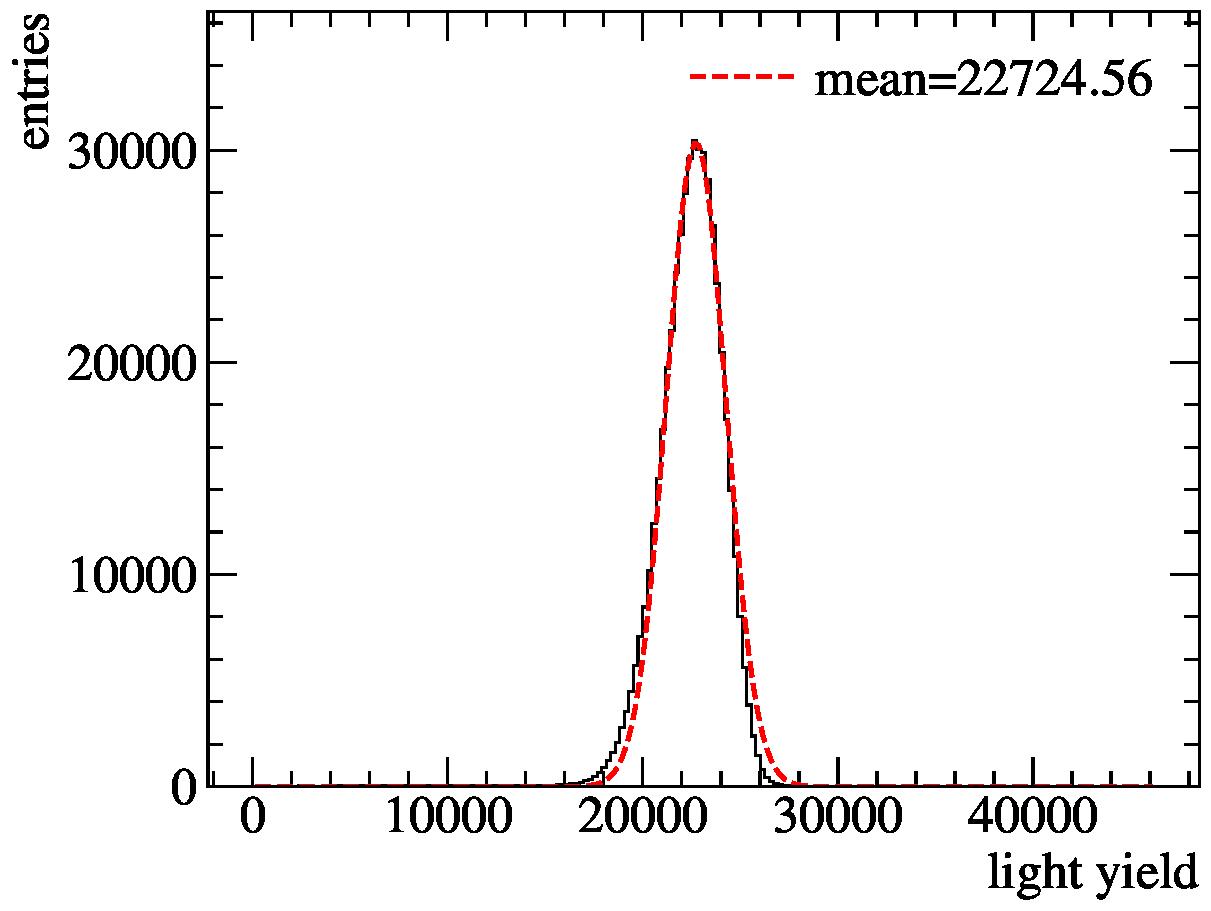
\includegraphics[width=\textwidth]{reconstruction/emmisionProfile/yield_gauss_fit_20.pdf}
		\caption{An example of Gaussian fit for light yield.}
		\label{fig:yield_gauss_fit}
	\end{subfigure}
	\hfill
	\begin{subfigure}{0.475\textwidth}
		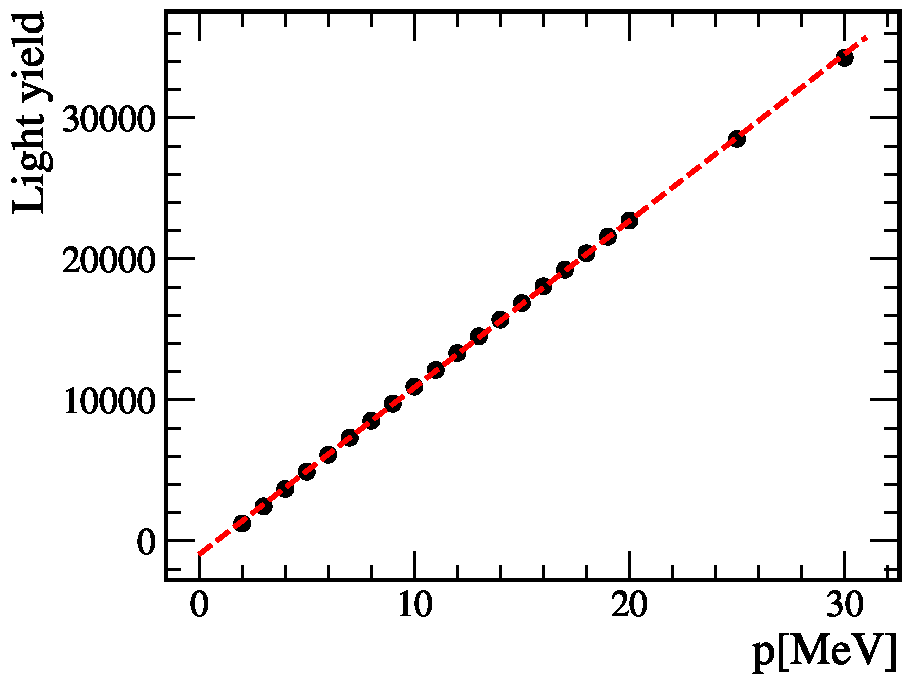
\includegraphics[width=\textwidth]{reconstruction/emmisionProfile/phip.pdf}
		\caption{\SI{5}{MeV} electron}
		\label{fig:yield_fit}
	\end{subfigure}
	\caption{The relationship of emission probability with $s$ and .}
\end{figure}

\subsection{The calculation of direct light}
After establishing the coordinate system, we can readily determine the number of photons received by a specific PMT when an electron is incident.
\begin{equation}
	\mu_{\mathrm{dir}}=\int ds g(p,s,\cos\theta)\phi(p)\Omega(R)T(R)\epsilon(\eta)
	\label{equ:directLight}
\end{equation}
\begin{itemize}
	\item $R$ is the distance between the position of electron and the PMT.
	\item $\Omega(R)$ is the solid angle factor of PMT.
	\item $T(R)$ is the light transmission factor.
	\item $\epsilon(\eta)$ is the PMT angular acceptance of PMT, and $\eta$ is the incident angle of light when captured by PMT.
\end{itemize}

\subsubsection{The solid angle factor}
The main PMTs employed in JUNO are 20-inch with a radius of $a=SI{0.622}{m}$. And we can calculate the solid angle of PMT by Eq.~\eqref{equ:solid}.
\begin{equation}
	\Omega(R)=\frac{\pi a^2}{4\pi(R^2+a^2)}\times (4\pi)=\frac{\pi a^2}{R^2+a^2}
	\label{equ:solid}
\end{equation}
In this approximation, the geometric shape of the PMT is ignored and approximated by a circular wafer. This approximation remains valid only when PMTs are sufficiently distant from the particle. In JUNO, PMTs are mounted at around \SI{19.5}{m} , while our region of interest lies within \SI{17.7}{m}. Based on SK's experience, the approximation holds effectively at radial distances $R > \SI{1.5}{m}$.

\subsubsection{The transmission factor}
In our work, we just use Eq.~\eqref{eq:att}, and the attenuation length $L^{a}$ is \SI{75}{m}.
\begin{equation}
	T(R) = \exp(-R/L^{a})
	\label{eq:att}
\end{equation}

\subsubsection{PMT angular accptance}
$\epsilon(\cos\eta)$ serves as a correction term for the approximation of the PMT wafer, describing the probability of photons being received by the PMT when incident from different directions. We extracted the particles at the same distance from the PMT in the simulation and counted the number of photons received by the PMT, as shown in Fig.~\ref{fig:eta_stat}. We performed a "normalization" calculation of the probability using the number of photons directly incident on the PMT, as shown in Fig.~\ref{fig:cd_norm} and \ref{fig:buffer_norm}. Then we extracted the probability distributions at different $\cos\eta$ values and fitted them with a Gaussian distribution, as shown in Fig.~\ref{fig:eta_gauss_fit}. Thus, we obtained the variation curve of $\epsilon(\cos\eta)$ and fitted it with a polynomial, as illustrated in Fig.~\ref{fig:eta_fit}. Whether it is in CD or buffer, a cut-off point can be observed. This is due to the mutual occlusion between the boundary of the detector and the PMT.

\begin{figure}[htbp]
	\centering
	\begin{subfigure}{0.475\textwidth}
		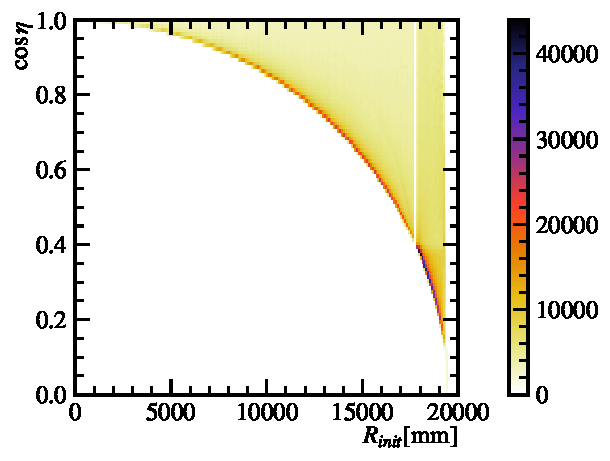
\includegraphics[page=1, width=\textwidth]{reconstruction/eta/fig.pdf}
		\caption{}
		\label{fig:eta_init}
	\end{subfigure}
	\hfill
	\begin{subfigure}{0.475\textwidth}
		\includegraphics[page=2, width=\textwidth]{reconstruction/eta/fig.pdf}
		\caption{}
		\label{fig:eta_R}
	\end{subfigure}
	\caption{\subref{fig:eta_init} is the position distribution, $R_{init}$ is the initial position of \SI{4}{MeV} electron.The boundary of the detector is at \SI{17.7}{m}. There is an acrylic spherical shell with a thickness of \SI{12}{cm}. The area between 17.7 and \SI{19.5}{m} is the buffer.
		\subref{fig:eta_R} shows the relationship between $R$ and $\cos\eta$. The boundary of the two distributions is the acrylic spherical shell.}
	\label{fig:eta_stat}
\end{figure}

\begin{figure}[htbp]
	\centering
	\begin{subfigure}{0.475\textwidth}
		\includegraphics[page=3, width=\textwidth]{reconstruction/eta/fig.pdf}
		\caption{}
		\label{fig:cd_norm}
	\end{subfigure}
	\hfill
	\begin{subfigure}{0.475\textwidth}
		\includegraphics[page=4, width=\textwidth]{reconstruction/eta/fig.pdf}
		\caption{}
		\label{fig:buffer_norm}
	\end{subfigure}
	\hfill
	\begin{subfigure}{0.475\textwidth}
		\includegraphics[page=45, width=\textwidth]{reconstruction/eta/cd.pdf}
		\caption{}
		\label{fig:eta_gauss_fit}
	\end{subfigure}
	\caption{\subref{fig:cd_norm} and \subref{fig:buffer_norm} are the normalized probability distribution. \subref{fig:eta_gauss_fit} is an example of Gaussian fit.}
	\label{fig:eta_gassian_fit}
\end{figure}

\begin{figure}[htbp]
	\centering
	\begin{subfigure}{0.475\textwidth}
		\includegraphics[page=1, width=\textwidth]{reconstruction/eta/fit.pdf}
		\caption{}
		\label{fig:eta_cd}
	\end{subfigure}
	\hfill
	\begin{subfigure}{0.475\textwidth}
		\includegraphics[page=2, width=\textwidth]{reconstruction/eta/fit.pdf}
		\caption{}
		\label{fig:eta_buffer}
	\end{subfigure}
	\caption{The relationship between acceptance~$\epsilon$ and $\cos\eta$ of when event in CD~\subref{fig:eta_cd} and in buffer~\subref{fig:eta_buffer}. }
	\label{fig:eta_fit}
\end{figure}

\subsubsection{The prediction of direct light}
For a single photon, we can combine its propagation process and the process of being captured by the PMT and define it as the photon reception function \(J=\Omega(R)T(R)\epsilon(\eta)\). Given the vertex and direction, this propagation process is only related to the generation position of the photon, that is, the distance from the photon generation point to the exit point when the photon is generated. We can write \(J\) as a function of \(s\) and perform a polynomial expansion, retaining the second-order approximation, as Eq.~\eqref{eq:jsApp} and the approximate performance is as shown in Fig.~\ref{fig:js}. Under this approximation, we can select 3 points to calculate the line. In the algorithm implementation, this can be quickly solved through methods such as matrix inversion.
\begin{equation}
	J(s)=\Omega(R)T(R)\epsilon(\eta)\approx j_0 + j_1s+j_2s^2
	\label{eq:jsApp}
\end{equation}

\begin{figure}
	\begin{center}
		\includegraphics[width=0.6\textwidth]{reconstruction/js.pdf}
	\end{center}
	\caption{An example of second-order approximation to calculate $J(s)$.}
	\label{fig:js}
\end{figure}
Thus far, we can decouple the process of photon generation from the process of photon capture, as shown in Eq.~\eqref{eq:mudir}.
\begin{equation}
	\begin{aligned}
		\mu_{\mathrm{dir}} & =\int ds g(p,s,\cos\theta)\phi(p)\Omega(R)T(R)\epsilon(\eta) \\
		                   & \approx \int ds g(p,s,\cos\theta)\phi(p)(j_0 + j_1s+j_2s^2)  \\
		                   & =\phi(p)(I_0j_0+I_1j_1+I_2j_2)                               \\
	\end{aligned}
	\label{eq:mudir}
\end{equation}
Where $I_i = \int ds g(p,s,\cos\theta)s^i$ is a function of $p, R, \cos\theta$ and represents the emission proportion of Cherenkov photons at a certain relative position. We can complete this integral calculation before the reconstruction.
Due to the relatively large differences in the integration range and emission spectrum at different momenta, we calculate the value of \(I\) for each momentum. Then, we perform a polynomial approximation fitting for momentum and \(I\), as shown in Fig.~\ref{fig:I_fit}. We create a grid with the fitting coefficients in terms of \(R\) and \(\cos\theta\). During the reconstruction process, by looking up different values of \(R\) and \(\cos\theta\) and invoking the corresponding polynomials for calculation, the reconstruction efficiency can be significantly improved.


\section{The Fast reconstruction~(FRE) of the JUNO water-phase}

\section{The parameters definition}
\subsection{The energy related parameters}
For a more accurate description, we define several parameters as follows.
\begin{itemize}
	\item $n_{10}$: The maximum count of residual time $t_{res}$ within a
	      \SI{10}{\nano s} bin width
	\item $n_{b}$: The average count of $t_{res}$ in [-20, -10] and
		      [30,40]\si{\nano s}.
	\item $n_{20}$: The total count of $t_{res}$ in [-20, 20]\si{\nano s},
	      \textbf{primary measure of energy}.
	\item $n_c$: The count of $\cos\theta$ in [0.65, 0.85], and the definition of $\theta$ is shown in Fig.~\ref{Fig:Coordinate}.
\end{itemize}

\begin{figure}[htbp]
	\centering
	\begin{subfigure}{0.5\textwidth}
		\centering
		\includegraphics[width=0.9\linewidth]{reconstruction/parameters_Define/tresCount.pdf}
		\caption{The distribution of $t_{res}$.}
		\label{fig:n20def}
	\end{subfigure}% 
	\begin{subfigure}{0.5\textwidth}
		\centering
		\includegraphics[width=0.9\linewidth]{reconstruction/parameters_Define/cosCount.pdf}
		\caption{The distribution of $\cos\theta$.}
		\label{fig:nc}
	\end{subfigure}
	\caption{The definition of parameters related to energy.}
	\label{fig:dual}
\end{figure}

\subsection{The parameters for reconstruction quality}
There exist two types of background, which can exert a significant impact on our analysis. These include the trigger stemming from pure dark noise and the events originating from PMT radioactivity. To eliminate these backgrounds, we introduce several parameters. To comprehensively assess the performance of each parameter, we simulate the uniform distribution of \SI{2.2}{MeV} Gamma, radioactive events from PMTs, and dark noise trigger events within the detector. Subsequently, reconstruction is performed following the MM trigger.

\subsubsection{Kurtosis test~($k$)}
The value obtained from the Kurtosis test on the residual time distribution is employed to assess the quality of the signal. In the case where the trigger originates from dark noise, the value should be -1.

\subsubsection{Akaike Information Criterion~(AIC)~$\delta A$}
AIC is frequently employed in model selection. In the context of reconstruction, it is utilized to determine whether the trigger originates from noise or a physical event. This Criterion is defined as Eq.~\eqref{eq:aic}
\begin{equation}
	\begin{aligned}
		 & \text{AIC}_v = -2 \ln \mathcal{L}_v + 2k_p \\
		 & \text{AIC}_0 = -2 \ln \mathcal{L}_0
	\end{aligned}
	\label{eq:aic}
\end{equation}
Where $\mathcal{L}$ represents the likelihood of the event with a single vertex, and $k_p$ denotes the number of reconstructed parameters. During the reconstruction process, we also calculate the likelihood of non-vertex events~($\mathcal{L}_0$). In this scenario, we can obtain the AIC criterion:
\begin{equation}
	\delta A = AIC_v - AIC_0 = 14 - 2\ln \mathcal{L}_v + \ln \mathcal{L}_0
	\label{eq:daic}
\end{equation}
By comparing $\delta A$ of dark noise events and \SI{2.2}{MeV} Gamma events, it can be seen that most dark noise events are eliminated, while less than \SI{10}{\%} of Gamma events are removed.
\begin{figure}
	\centering
	\includegraphics[width=0.475\textwidth]{reconstruction/parameters_Define/AIC_per.pdf}
	\caption{There is obvious difference between dark noise and
		\SI{2.2}{MeV} Gamma. We can optimize it to remove dark noise events.}
\end{figure}

\subsubsection{The likelihood-energy combined Criterion~($LE$)}
We define the likelihood-energy combined criterion as $LE$, as Eq.~\eqref{eq:le}
\begin{equation}
	LE = -\ln \mathcal{L}/n_{20}
	\label{eq:le}
\end{equation}
This criterion is employed to eliminate events stemming from PMT radioactivity. When the cut $LE < 40$ is applied, over \SI{99.99}{\%} of the events from PMT radioactivity are removed, along with approximately \SI{30}{\%} of the \SI{2.2}{MeV} Gamma.
\begin{figure}[htbp]
	\centering
	\begin{subfigure}{0.32\textwidth} % 宽度调整为0.32(留出间隙)
		\centering
		\includegraphics[page=3, width=\linewidth]{reconstruction/parameters_Define/glass.pdf}
		\caption{\SI{2.2}{MeV} Gamma}
		\label{fig:glass3}
	\end{subfigure}%
	\hfill
	\begin{subfigure}{0.32\textwidth}
		\centering
		\includegraphics[page=6, width=\linewidth]{reconstruction/parameters_Define/glass.pdf}
		\caption{PMT radioactivity}
		\label{fig:glass6}
	\end{subfigure}%
	\hfill
	\begin{subfigure}{0.32\textwidth}
		\centering
		\includegraphics[page=9, width=\linewidth]{reconstruction/parameters_Define/glass.pdf}
		\caption{dark noise events}
		\label{fig:glass9}
	\end{subfigure}
	\caption{The relationship between $\mathcal{L}$ and $n_{20}$.}
	\label{fig:glass_all}
\end{figure}

\subsubsection{The goodness of reconstruction~($G_{vd}$)}
When contemplating reconstruction, it is essential to assess the quality of both position and direction. In the case of a successfully reconstructed position, the residual time should be distributed as closely as feasible around zero. For precise direction reconstruction, PMTs adjacent to the Cherenkov ring ought to demonstrate uniform photon acceptance. In accordance with these criteria, we formulate the following two goodness metrics, presented as Eq.~\eqref{eq:goodness}. Finally, we combine these two metrics to obtain the overall goodness of reconstruction, denoted as $G_{vd}=g_v^2-g_d^2$.
\begin{equation}
	\begin{aligned}
		g_v & = \frac{\sum e^{-0.5(t_{res}/w)^2} e^{-0.5(t_{res}/\sigma)^2}}{\sum e^{-0.5(t_{res}/w)^2}}                                \\
		g_d & = \frac{1}{2\pi} \left[ \max\left( \phi_i - \frac{2i\pi}{N} \right) - \min\left( \phi_i - \frac{2i\pi}{N} \right) \right] \\
	\end{aligned}
	\label{eq:goodness}
\end{equation}
\begin{itemize}
	\item $w$ and $\sigma$: in this work, $w=\SI{20}{ns}$ and $\sigma$ is the TTS of PMT.
	\item $g_v$: The goodness of position reconstruction.
	\item $g_d$: The goodness of direction, describes the uniformity of the azimuthal angle distribution, as shown in Fig.~\ref{fig:goodness}.
\end{itemize}
\begin{figure}
	\centering
	\includegraphics[width=0.475\textwidth]{reconstruction/parameters_Define/gd.pdf}
	\caption{The definition of azimuthal angle in the goodness of direction calculation.}
	\label{fig:goodness}
\end{figure}

\subsection{In the dector simulation}
\subsection{In the electronic simulation}


% 参考文献
\bibliography{ref/refs}  % 参考文献使用 BibTeX 编译
% \printbibliography       % 参考文献使用 BibLaTeX 编译

% 附录
\appendix
% % !TeX root = ../thuthesis-example.tex

\begin{survey}
\label{cha:survey}

\title{Title of the Survey}
\maketitle


\tableofcontents


本科生的外文资料调研阅读报告。


\section{Figures and Tables}

\subsection{Figures}

An example figure in appendix (Figure~\ref{fig:appendix-survey-figure}).

\begin{figure}
  \centering
  \includegraphics[width=0.6\linewidth]{example-image-a.pdf}
  \caption{Example figure in appendix}
  \label{fig:appendix-survey-figure}
\end{figure}


\subsection{Tables}

An example table in appendix (Table~\ref{tab:appendix-survey-table}).

\begin{table}
  \centering
  \caption{Example table in appendix}
  \begin{tabular}{ll}
    \toprule
    File name       & Description                                         \\
    \midrule
    thuthesis.dtx   & The source file including documentation and comments \\
    thuthesis.cls   & The template file                                   \\
    thuthesis-*.bst & BibTeX styles                                       \\
    thuthesis-*.bbx & BibLaTeX styles for bibliographies                  \\
    thuthesis-*.cbx & BibLaTeX styles for citations                       \\
    \bottomrule
  \end{tabular}
  \label{tab:appendix-survey-table}
\end{table}


\section{Equations}

An example equation in appendix (Equation~\eqref{eq:appendix-survey-equation}).
\begin{equation}
  \frac{1}{2 \uppi \symup{i}} \int_\gamma f = \sum_{k=1}^m n(\gamma; a_k) \mathscr{R}(f; a_k)
  \label{eq:appendix-survey-equation}
\end{equation}


\section{Citations}

Example\cite{dupont1974bone} citations\cite{merkt1995rotational} in appendix
\cite{dupont1974bone,merkt1995rotational}.


% 默认使用正文的参考文献样式;
% 如果使用 BibTeX,可以切换为其他兼容 natbib 的 BibTeX 样式。
\bibliographystyle{unsrtnat}
% \bibliographystyle{IEEEtranN}

% 默认使用正文的参考文献 .bib 数据库;
% 如果使用 BibTeX,可以改为指定数据库,如 \bibliography{ref/refs}。
\printbibliography

\end{survey}
       % 本科生:外文资料的调研阅读报告
% % !TeX root = ../thuthesis-example.tex

\begin{translation}
\label{cha:translation}

\title{书面翻译题目}
\maketitle

\tableofcontents


本科生的外文资料书面翻译。


\section{图表示例}

\subsection{图}

附录中的图片示例(图~\ref{fig:appendix-translation-figure})。

\begin{figure}
  \centering
  \includegraphics[width=0.6\linewidth]{example-image-a.pdf}
  \caption{附录中的图片示例}
  \label{fig:appendix-translation-figure}
\end{figure}


\subsection{表格}

附录中的表格示例(表~\ref{tab:appendix-translation-table})。

\begin{table}
  \centering
  \caption{附录中的表格示例}
  \begin{tabular}{ll}
    \toprule
    文件名          & 描述                         \\
    \midrule
    thuthesis.dtx   & 模板的源文件,包括文档和注释 \\
    thuthesis.cls   & 模板文件                     \\
    thuthesis-*.bst & BibTeX 参考文献表样式文件    \\
    thuthesis-*.bbx & BibLaTeX 参考文献表样式文件  \\
    thuthesis-*.cbx & BibLaTeX 引用样式文件        \\
    \bottomrule
  \end{tabular}
  \label{tab:appendix-translation-table}
\end{table}


\section{数学公式}

附录中的数学公式示例(公式\eqref{eq:appendix-translation-equation})。
\begin{equation}
  \frac{1}{2 \uppi \symup{i}} \int_\gamma f = \sum_{k=1}^m n(\gamma; a_k) \mathscr{R}(f; a_k)
  \label{eq:appendix-translation-equation}
\end{equation}


\section{文献引用}

附录\cite{dupont1974bone}中的参考文献引用\cite{merkt1995rotational}示例
\cite{dupont1974bone,merkt1995rotational}。


\appendix

\section{附录}

附录的内容。


% 书面翻译的参考文献
% 默认使用正文的参考文献样式;
% 如果使用 BibTeX,可以切换为其他兼容 natbib 的 BibTeX 样式。
\bibliographystyle{unsrtnat}
% \bibliographystyle{IEEEtranN}

% 默认使用正文的参考文献 .bib 数据库;
% 如果使用 BibTeX,可以改为指定数据库,如 \bibliography{ref/refs}。
\printbibliography

% 书面翻译对应的原文索引
\begin{translation-index}
  \nocite{mellinger1996laser}
  \nocite{bixon1996dynamics}
  \nocite{carlson1981two}
  \bibliographystyle{unsrtnat}
  \printbibliography
\end{translation-index}

\end{translation}
  % 本科生:外文资料的书面翻译
% % !TeX root = ../thuthesis-example.tex

\chapter{补充内容}

附录是与论文内容密切相关、但编入正文又影响整篇论文编排的条理和逻辑性的资料,例如某些重要的数据表格、计算程序、统计表等,是论文主体的补充内容,可根据需要设置。

附录中的图、表、数学表达式、参考文献等另行编序号,与正文分开,一律用阿拉伯数字编码,
但在数码前冠以附录的序号,例如“图~\ref{fig:appendix-figure}”,
“表~\ref{tab:appendix-table}”,“式\eqref{eq:appendix-equation}”等。


\section{插图}

% 附录中的插图示例(图~\ref{fig:appendix-figure})。

\begin{figure}
  \centering
  \includegraphics[width=0.6\linewidth]{example-image-a.pdf}
  \caption{附录中的图片示例}
  \label{fig:appendix-figure}
\end{figure}


\section{表格}

% 附录中的表格示例(表~\ref{tab:appendix-table})。

\begin{table}
  \centering
  \caption{附录中的表格示例}
  \begin{tabular}{ll}
    \toprule
    文件名          & 描述                         \\
    \midrule
    thuthesis.dtx   & 模板的源文件,包括文档和注释 \\
    thuthesis.cls   & 模板文件                     \\
    thuthesis-*.bst & BibTeX 参考文献表样式文件    \\
    thuthesis-*.bbx & BibLaTeX 参考文献表样式文件  \\
    thuthesis-*.cbx & BibLaTeX 引用样式文件        \\
    \bottomrule
  \end{tabular}
  \label{tab:appendix-table}
\end{table}


\section{数学表达式}

% 附录中的数学表达式示例(式\eqref{eq:appendix-equation})。
\begin{equation}
  \frac{1}{2 \uppi \symup{i}} \int_\gamma f = \sum_{k=1}^m n(\gamma; a_k) \mathscr{R}(f; a_k)
  \label{eq:appendix-equation}
\end{equation}


\section{文献引用}

附录\cite{dupont1974bone}中的参考文献引用\cite{zhengkaiqing1987}示例
\cite{dupont1974bone,zhengkaiqing1987}。

\printbibliography


% 其他部分
% \backmatter

% 致谢
% % !TeX root = ../thuthesis-example.tex

\begin{acknowledgements}
  衷心感谢导师×××教授和物理系××副教授对本人的精心指导。他们的言传身教将使我终生受益。

  在美国麻省理工学院化学系进行九个月的合作研究期间,承蒙 Robert Field 教授热心指导与帮助,不胜感激。

  感谢×××××实验室主任×××教授,以及实验室全体老师和同窗们学的热情帮助和支持!

  本课题承蒙国家自然科学基金资助,特此致谢。
\end{acknowledgements}


% 声明
% 各类开题报告通常不需要
% \statement[page-style=empty]  % 编译生成的声明页默认不含页眉页脚,以避免页码变化带来问题
% 在提交终稿时,插入签字后的扫描件 scan-statement.pdf,并添加页眉页脚
% \statement[page-style=plain, file=scan-statement.pdf]
% 如确实需要在电子版中直接页眉页脚,则使用
% \statement[page-style=plain]

% 个人简历、在学期间完成的相关学术成果
% 本科生可以附个人简历,也可以不附个人简历
% % !TeX root = ../thuthesis-example.tex

\begin{resume}

  \section*{个人简历}

  197× 年 ×× 月 ×× 日出生于四川××县。

  1992 年 9 月考入××大学化学系××化学专业,1996 年 7 月本科毕业并获得理学学士学位。

  1996 年 9 月免试进入清华大学化学系攻读××化学博士至今。


  \section*{在学期间完成的相关学术成果}

  \subsection*{学术论文}

  \begin{achievements}
    \item Yang Y, Ren T L, Zhang L T, et al. Miniature microphone with silicon-based ferroelectric thin films[J]. Integrated Ferroelectrics, 2003, 52:229-235.
    \item 杨轶, 张宁欣, 任天令, 等. 硅基铁电微声学器件中薄膜残余应力的研究[J]. 中国机械工程, 2005, 16(14):1289-1291.
    \item 杨轶, 张宁欣, 任天令, 等. 集成铁电器件中的关键工艺研究[J]. 仪器仪表学报, 2003, 24(S4):192-193.
    \item Yang Y, Ren T L, Zhu Y P, et al. PMUTs for handwriting recognition. In press[J]. (已被Integrated Ferroelectrics录用)
  \end{achievements}


  \subsection*{专利}

  \begin{achievements}
    \item 任天令, 杨轶, 朱一平, 等. 硅基铁电微声学传感器畴极化区域控制和电极连接的方法: 中国, CN1602118A[P]. 2005-03-30.
    \item Ren T L, Yang Y, Zhu Y P, et al. Piezoelectric micro acoustic sensor based on ferroelectric materials: USA, No.11/215, 102[P]. (美国发明专利申请号.)
  \end{achievements}

\end{resume}



% 本科生格式:

% \begin{resume}
%   \section*{学术论文}
%
%   \begin{achievements}
%     \item ZHOU R, HU C, OU T, et al. Intelligent GRU-RIC Position-Loop
%       Feedforward Compensation Control Method with Application to an
%       Ultraprecision Motion Stage[J], IEEE Transactions on Industrial
%       Informatics, 2024, 20(4): 5609-5621.
%
%     \item 杨轶, 张宁欣, 任天令, 等. 硅基铁电微声学器件中薄膜残余应力的研究[J].
%       中国机械工程, 2005, 16(14):1289-1291.
%
%     \item YANG Y, REN T L, ZHU Y P, et al. PMUTs for handwriting recognition.
%       In press[J]. (已被Integrated Ferroelectrics录用)
%
%   \end{achievements}
%
%
%   \section*{专利}
%
%   \begin{achievements}
%     \item 胡楚雄, 付宏, 朱煜, 等. 一种磁悬浮平面电机: ZL202011322520.6[P]. 2022-04-01.
%
%     \item REN T L, YANG Y, ZHU Y P, et al. Piezoelectric micro acoustic sensor
%       based on ferroelectric materials: No.11/215, 102[P]. (美国发明专利申请号.)
%
%   \end{achievements}
% \end{resume}


% 指导教师/指导小组评语
% 本科生不需要
% % !TeX root = ../thuthesis-example.tex

\begin{comments}
% \begin{comments}[name = {指导小组评语}]
% \begin{comments}[name = {Comments from Thesis Supervisor}]
% \begin{comments}[name = {Comments from Thesis Supervision Committee}]

  论文提出了……

\end{comments}


% 答辩委员会决议书
% 本科生不需要
% % !TeX root = ../thuthesis-example.tex

\begin{resolution}

  论文提出了……

  论文取得的主要创新性成果包括:

  1. ……

  2. ……

  3. ……

  论文工作表明作者在×××××具有×××××知识,具有××××能力,论文××××,答辩××××。

  答辩委员会表决,(×票/一致)同意通过论文答辩,并建议授予×××(姓名)×××(门类)学博士/硕士学位。

\end{resolution}


% 本科生的综合论文训练记录表(扫描版)
% \record{file=scan-record.pdf}

\end{document}
